\documentclass[8pt,b5paper,twoside,openright]{book}
%\usepackage[left=2cm,right=2cm,top=2cm,bottom=3cm]{geometry}
\usepackage[
  top=2cm,
  bottom=3cm,
  left=2cm,
  right=2cm,
  marginparwidth=0cm,
  marginparsep=0cm,
  headheight=13.6pt]{geometry}

\usepackage{icthesis}
\usepackage{graphicx}
\usepackage{verbatim}
\usepackage{latexsym}
\usepackage{mathchars}
\usepackage{setspace}

\setlength{\parskip}{\medskipamount}  % a little space before a \par
\setlength{\parindent}{0pt}	      % don't indent first lines of paragraphs
%UHEAD.STY  If this is included after \documentstyle{report}, it adds
% an underlined heading style to the LaTeX report style.
% \pagestyle{uheadings} will put underlined headings at the top
% of each page. The right page headings are the Chapter titles and
% the left page titles are supplied by \def\lefthead{text}.

% Ted Shapin, Dec. 17, 1986

\makeatletter
\def\chapapp2{Chapter}

\def\appendix{\par
 \setcounter{chapter}{0}
 \setcounter{section}{0}
 \def\chapapp2{Appendix}
 \def\@chapapp{Appendix}
 \def\thechapter{\Alph{chapter}}}

\def\ps@uheadings{\let\@mkboth\markboth
% modifications
\def\@oddhead{\protect\underline{\protect\makebox[\textwidth][l]
		{\sl\rightmark\hfill\rm\thepage}}}
\def\@oddfoot{}
\def\@evenfoot{}
\def\@evenhead{\protect\underline{\protect\makebox[\textwidth][l]
		{\rm\thepage\hfill\sl\leftmark}}}
% end of modifications
\def\chaptermark##1{\markboth {\ifnum \c@secnumdepth >\m@ne
 \chapapp2\ \thechapter. \ \fi ##1}{}}%
\def\sectionmark##1{\markright {\ifnum \c@secnumdepth >\z@
   \thesection. \ \fi ##1}}}
\makeatother
%%From: marcel@cs.caltech.edu (Marcel van der Goot)
%%Newsgroups: comp.text.tex
%%Subject: illegal modification of boxit.sty
%%Date: 28 Feb 92 01:10:02 GMT
%%Organization: California Institute of Technology (CS dept)
%%Nntp-Posting-Host: andromeda.cs.caltech.edu
%%
%%
%%Quite some time ago I posted a file boxit.sty; maybe it made it
%%to some archives, although I don't recall submitting it. It defines
%%	\begin{boxit}
%%	...
%%	\end{boxit}
%%to draw a box around `...', where the `...' can contain other
%%environments (e.g., a verbatim environment). Unfortunately, it had
%%a problem: it did not work if you used it in paragraph mode, i.e., it
%%only worked if there was an empty line in front of \begin{boxit}.
%%Luckily, that is easily corrected.
%%
%%HOWEVER, apparently someone noticed the problem, tried to correct it,
%%and then distributed this modified version. That would be fine with me,
%%except that:
%%1. There was no note in the file about this modification, it only has my
%%   name in it.
%%2. The modification is wrong: now it only works if there is *no* empty
%%   line in front of \begin{boxit}. In my opinion this bug is worse than
%%   the original one.
%%
%%In particular, the author of this modification tried to force an empty
%%line by inserting a `\\' in the definition of \Beginboxit. If you have
%%a version of boxit.sty with a `\\', please delete it. If you have my
%%old version of boxit.sty, please also delete it. Below is an improved
%%version.
%%
%%Thanks to Joe Armstrong for drawing my attention to the bug and to the
%%illegal version.
%%
%%                                          Marcel van der Goot
%% .---------------------------------------------------------------
%% | Blauw de viooltjes,                    marcel@cs.caltech.edu
%% |    Rood zijn de rozen;
%% | Een rijm kan gezet
%% |    Met plaksel en dozen.
%% |


% boxit.sty
% version: 27 Feb 1992
%
% Defines a boxit environment, which draws lines around its contents.
% Usage:
%   \begin{boxit}
%	... (text you want to be boxed, can contain other environments)
%   \end{boxit}
%
% The width of the box is the width of the contents.
% The boxit* environment behaves the same, except that the box will be
% at least as wide as a normal paragraph.
%
% The reason for writing it this way (rather than with the \boxit#1 macro
% from the TeXbook), is that now you can box verbatim text, as in
%   \begin{boxit}
%   \begin{verbatim}
%   this better come out in boxed verbatim mode ...
%   \end{verbatim}
%   \end{boxit}
%
%						Marcel van der Goot
%						marcel@cs.caltech.edu
%

\def\Beginboxit
   {\par
    \vbox\bgroup
	   \hrule
	   \hbox\bgroup
		  \vrule \kern1.2pt %
		  \vbox\bgroup\kern1.2pt
   }

\def\Endboxit{%
			      \kern1.2pt
		       \egroup
		  \kern1.2pt\vrule
		\egroup
	   \hrule
	 \egroup
   }	

\newenvironment{boxit}{\Beginboxit}{\Endboxit}
\newenvironment{boxit*}{\Beginboxit\hbox to\hsize{}}{\Endboxit}
\pagestyle{empty}

%Trying font
\usepackage{baskervillef}


\makeatletter  %to avoid error messages generated by "\@". Makes Latex treat "@" like a letter

\linespread{0.5}
\def\submitdate#1{\gdef\@submitdate{#1}}

\def\maketitle{
  \begin{titlepage}{
   \vskip 0.3in
    %\linespread{1.5}
    \Large Orchestration of Distributed LOFAR Workflows 
    %\linebreak
%    Leiden Observatory and  \\
    %\linebreak
 %   Leiden Institute of Advanced Computer Science
    \rm
    \vskip 1.3in
  %  \Large \bf  \par
  }
  \pagenumbering{roman}                                                                                                              
  \vskip 0.6in
  \par
  {\Large PROEFSCHRIFT}
  \vskip 1.1in
  \par
  ter verkrijging van 
  \linebreak
  de graad van Doctor aan de Universiteit Leiden
      \linebreak
      op gezag van de Rector Magnificus Prof. mr. C.J.J.M Stolker, 
      \linebreak
      volgens besluit van het College voor Promoties
      \linebreak
      te verdedigen op maandag 9 December 2019 klokke 15:00 uur
      \linebreak
      \vskip 1.2in
      door
      \linebreak 
      Alexandar Plamenov Mechev
      \linebreak
      geboren te Sofia, Bulgarije 
      \linebreak
      in 1989
  \vfil
  \end{titlepage}
}

\def\titlepage{
  \newpage
  \centering
  \linespread{1}
  \normalsize
  \vbox to \vsize\bgroup\vbox to 9in\bgroup
}
\def\endtitlepage{
  \par
  \kern 0pt
  \egroup
  \vss
  \egroup
%  \cleardoublepage
}

\def\abstract{
  \begin{center}{
    \large\bf Abstract}
  \end{center}
  \small
  %\def\baselinestretch{1.5}
  \linespread{1.5}
  \normalsize
}
\def\endabstract{
  \par
}

\newenvironment{thesisacknowledgements}{
  \cleardoublepage
  \begin{center}{
    \large \bf Acknowledgements}
  \end{center}
  \small
  \linespread{1.5}
  \normalsize
}{\cleardoublepage}
\def\endthesisacknowledgements{
  \par
}

\newenvironment{thesisdedication}{
  \cleardoublepage
  \begin{center}{
    \large \bf Dedication}
  \end{center}
  \small
  \linespread{1.5}
  \normalsize
}{\cleardoublepage}
\def\endthesisdedication{
  \par
}

\def\preface{
    \pagenumbering{roman}
    \pagestyle{plain}
    \onehalfspacing
}

\def\body{
    \cleardoublepage    
    \pagestyle{uheadings}
    \pdfbookmark[section]{\contentsname}{toc}
    \pdfbookmark[subsection]{Chapters}{chaptertoc}
    \setcounter{tocdepth}{1}
    \tableofcontents

    \pagestyle{plain}
    \cleardoublepage
    \pagestyle{uheadings}
    \pdfbookmark[subsection]{Tables}{tabletoc} 
    \listoftables
    \pagestyle{plain}
    \onehalfspacing
    \normalsize
    \cleardoublepage
    \pagestyle{uheadings}
    \pdfbookmark[subsection]{Figures}{figuretoc}
    \listoffigures
    \pagestyle{plain}
    \cleardoublepage
    \pagestyle{uheadings}
    \pagenumbering{arabic}
   
    \normalsize
    \onehalfspacing 
    \fontsize{11}{12}\selectfont
}
%%%%%%%%
\def\ead{\@ifnextchar[{\@uad}{\@ead}}
\gdef\@ead#1{\bgroup\def\_{\string\underscorechar\space}%
  \def\{{\string\lbracechar\space}%
   \def~{\hashchar\space}%
   \def\}{\string\rbracechar\space}%
   \edef\tmp{\the\@eadauthor}
   \immediate\write\@auxout{\string\emailauthor
     {#1}{\expandafter\strip@prefix\meaning\tmp}}%
  \egroup
}
\newcounter{ead}
\makeatother  %to avoid error messages generated by "\@". Makes Latex treat "@" like a letter


\newcommand{\ipc}{{\sf ipc}}

\newcommand{\Prob}{\bbbp}
\newcommand{\Real}{\bbbr}
\newcommand{\real}{\Real}
\newcommand{\Int}{\bbbz}
\newcommand{\Nat}{\bbbn}

\newcommand{\NN}{{\sf I\kern-0.14emN}}   % Natural numbers
\newcommand{\ZZ}{{\sf Z\kern-0.45emZ}}   % Integers
\newcommand{\QQQ}{{\sf C\kern-0.48emQ}}   % Rational numbers
\newcommand{\RR}{{\sf I\kern-0.14emR}}   % Real numbers
\newcommand{\KK}{{\cal K}}
\newcommand{\OO}{{\cal O}}
\newcommand{\AAA}{{\bf A}}
\newcommand{\HH}{{\bf H}}
\newcommand{\II}{{\bf I}}
\newcommand{\LL}{{\bf L}}
\newcommand{\PP}{{\bf P}}
\newcommand{\PPprime}{{\bf P'}}
\newcommand{\QQ}{{\bf Q}}
\newcommand{\UU}{{\bf U}}
\newcommand{\UUprime}{{\bf U'}}
\newcommand{\zzero}{{\bf 0}}
\newcommand{\ppi}{\mbox{\boldmath $\pi$}}
\newcommand{\aalph}{\mbox{\boldmath $\alpha$}}
\newcommand{\bb}{{\bf b}}
\newcommand{\ee}{{\bf e}}
\newcommand{\mmu}{\mbox{\boldmath $\mu$}}
\newcommand{\vv}{{\bf v}}
\newcommand{\xx}{{\bf x}}
\newcommand{\yy}{{\bf y}}
\newcommand{\zz}{{\bf z}}
\newcommand{\oomeg}{\mbox{\boldmath $\omega$}}
\newcommand{\res}{{\bf res}}
\newcommand{\cchi}{{\mbox{\raisebox{.4ex}{$\chi$}}}}
%\newcommand{\cchi}{{\cal X}}
%\newcommand{\cchi}{\mbox{\Large $\chi$}}

% Logical operators and symbols
\newcommand{\imply}{\Rightarrow}
\newcommand{\bimply}{\Leftrightarrow}
\newcommand{\union}{\cup}
\newcommand{\intersect}{\cap}
\newcommand{\boolor}{\vee}
\newcommand{\booland}{\wedge}
\newcommand{\boolimply}{\imply}
\newcommand{\boolbimply}{\bimply}
\newcommand{\boolnot}{\neg}
\newcommand{\boolsat}{\!\models}
\newcommand{\boolnsat}{\!\not\models}


\newcommand{\op}[1]{\mathrm{#1}}
\newcommand{\s}[1]{\ensuremath{\mathcal #1}}

% Properly styled differentiation and integration operators
\newcommand{\diff}[1]{\mathrm{\frac{d}{d\mathit{#1}}}}
\newcommand{\diffII}[1]{\mathrm{\frac{d^2}{d\mathit{#1}^2}}}
\newcommand{\intg}[4]{\int_{#3}^{#4} #1 \, \mathrm{d}#2}
\newcommand{\intgd}[4]{\int\!\!\!\!\int_{#4} #1 \, \mathrm{d}#2 \, \mathrm{d}#3}

% Large () brackets on different lines of an eqnarray environment
\newcommand{\Leftbrace}[1]{\left(\raisebox{0mm}[#1][#1]{}\right.}
\newcommand{\Rightbrace}[1]{\left.\raisebox{0mm}[#1][#1]{}\right)}

% Funky symobols for footnotes
\newcommand{\symbolfootnote}{\renewcommand{\thefootnote}{\fnsymbol{footnote}}}
% now add \symbolfootnote to the beginning of the document...

\newcommand{\normallinespacing}{\renewcommand{\baselinestretch}{1.5} \normalsize}
\newcommand{\mediumlinespacing}{\renewcommand{\baselinestretch}{1.2} \normalsize}
\newcommand{\narrowlinespacing}{\renewcommand{\baselinestretch}{1.0} \normalsize}
\newcommand{\bump}{\noalign{\vspace*{\doublerulesep}}}
\newcommand{\cell}{\multicolumn{1}{}{}}
\newcommand{\spann}{\mbox{span}}
\newcommand{\diagg}{\mbox{diag}}
\newcommand{\modd}{\mbox{mod}}
\newcommand{\minn}{\mbox{min}}
\newcommand{\andd}{\mbox{and}}
\newcommand{\forr}{\mbox{for}}
\newcommand{\EE}{\mbox{E}}

\newcommand{\deff}{\stackrel{\mathrm{def}}{=}}
\newcommand{\syncc}{~\stackrel{\textstyle \rhd\kern-0.57em\lhd}{\scriptstyle L}~}

\def\coop{\mbox{\large $\rhd\!\!\!\lhd$}}
\newcommand{\sync}[1]{\raisebox{-1.0ex}{$\;\stackrel{\coop}{\scriptscriptstyle
#1}\,$}}

\newtheorem{definition}{Definition}[chapter]
\newtheorem{theorem}{Theorem}[chapter]

\newcommand{\Figref}[1]{Figure~\ref{#1}}
\newcommand{\fig}[3]{
 \begin{figure}[!ht]
 \begin{center}
 \scalebox{#3}{\includegraphics{figs/#1.ps}}
 \vspace{-0.1in}
 \caption[ ]{\label{#1} #2}
 \end{center}
 \end{figure}
}

\newcommand{\figtwo}[8]{
 \begin{figure}
 \parbox[b]{#4 \textwidth}{
 \begin{center}
 \scalebox{#3}{\includegraphics{figs/#1.ps}}
 \vspace{-0.1in}
 \caption{\label{#1}#2}
 \end{center}
 }
 \hfill
 \parbox[b]{#8 \textwidth}{
 \begin{center}
 \scalebox{#7}{\includegraphics{figs/#5.ps}}
 \vspace{-0.1in}
 \caption{\label{#5}#6}
 \end{center}
 }
 \end{figure}
}

\newcommand\aj{\rmfamily{AJ}}% 
          % Astronomical Journal 
\newcommand\araa{\rmfamily{ARA\&A}}% 
          % Annual Review of Astron and Astrophys 
\newcommand\apj{\rmfamily{ApJ}}% 
          % Astrophysical Journal 
\newcommand\apjl{\rmfamily{ApJ}}% 
          % Astrophysical Journal, Letters 
\newcommand\apjs{\rmfamily{ApJS}}% 
          % Astrophysical Journal, Supplement 
\newcommand\ao{\rmfamily{Appl.~Opt.}}% 
          % Applied Optics 
\newcommand\apss{\rmfamily{Ap\&SS}}% 
          % Astrophysics and Space Science 
\newcommand\aap{\rmfamily{A\&A}}% 
          % Astronomy and Astrophysics 
\newcommand\aapr{\rmfamily{A\&A~Rev.}}% 
          % Astronomy and Astrophysics Reviews 
\newcommand\aaps{\rmfamily{A\&AS}}% 
          % Astronomy and Astrophysics, Supplement 
\newcommand\azh{\rmfamily{AZh}}% 
          % Astronomicheskii Zhurnal 
\newcommand\baas{\rmfamily{BAAS}}% 
          % Bulletin of the AAS 
\newcommand\jrasc{\rmfamily{JRASC}}% 
          % Journal of the RAS of Canada 
\newcommand\memras{\rmfamily{MmRAS}}% 
          % Memoirs of the RAS 
\newcommand\mnras{\rmfamily{MNRAS}}% 
          % Monthly Notices of the RAS 
\newcommand\pra{\rmfamily{Phys.~Rev.~A}}% 
          % Physical Review A: General Physics 
\newcommand\prb{\rmfamily{Phys.~Rev.~B}}% 
          % Physical Review B: Solid State 
\newcommand\prc{\rmfamily{Phys.~Rev.~C}}% 
          % Physical Review C 
\newcommand\prd{\rmfamily{Phys.~Rev.~D}}% 
          % Physical Review D 
\newcommand\pre{\rmfamily{Phys.~Rev.~E}}% 
          % Physical Review E 
\newcommand\prl{\rmfamily{Phys.~Rev.~Lett.}}% 
          % Physical Review Letters 
\newcommand\pasp{\rmfamily{PASP}}% 
          % Publications of the ASP 
\newcommand\pasj{\rmfamily{PASJ}}% 
          % Publications of the ASJ 
\newcommand\qjras{\rmfamily{QJRAS}}% 
          % Quarterly Journal of the RAS 
\newcommand\skytel{\rmfamily{S\&T}}% 
          % Sky and Telescope 
\newcommand\solphys{\rmfamily{Sol.~Phys.}}% 
          % Solar Physics 
\newcommand\sovast{\rmfamily{Soviet~Ast.}}% 
          % Soviet Astronomy 
\newcommand\ssr{\rmfamily{Space~Sci.~Rev.}}% 
          % Space Science Reviews 
\newcommand\zap{\rmfamily{ZAp}}% 
          % Zeitschrift fuer Astrophysik 
\newcommand\nat{\rmfamily{Nature}}% 
          % Nature 
\newcommand\iaucirc{\rmfamily{IAU~Circ.}}% 
          % IAU Cirulars 
\newcommand\aplett{\rmfamily{Astrophys.~Lett.}}% 
          % Astrophysics Letters 
\newcommand\apspr{\rmfamily{Astrophys.~Space~Phys.~Res.}}% 
          % Astrophysics Space Physics Research 
\newcommand\bain{\rmfamily{Bull.~Astron.~Inst.~Netherlands}}% 
          % Bulletin Astronomical Institute of the Netherlands 
\newcommand\fcp{\rmfamily{Fund.~Cosmic~Phys.}}% 
          % Fundamental Cosmic Physics 
\newcommand\gca{\rmfamily{Geochim.~Cosmochim.~Acta}}% 
          % Geochimica Cosmochimica Acta 
\newcommand\grl{\rmfamily{Geophys.~Res.~Lett.}}% 
          % Geophysics Research Letters 
\newcommand\jcp{\rmfamily{J.~Chem.~Phys.}}% 
          % Journal of Chemical Physics 
\newcommand\jgr{\rmfamily{J.~Geophys.~Res.}}% 
          % Journal of Geophysics Research 
\newcommand\jqsrt{\rmfamily{J.~Quant.~Spec.~Radiat.~Transf.}}% 
          % Journal of Quantitiative Spectroscopy and Radiative Trasfer 
\newcommand\memsai{\rmfamily{Mem.~Soc.~Astron.~Italiana}}% 
          % Mem. Societa Astronomica Italiana 
\newcommand\nphysa{\rmfamily{Nucl.~Phys.~A}}% 
          % Nuclear Physics A 
\newcommand\physrep{\rmfamily{Phys.~Rep.}}% 
          % Physics Reports 
\newcommand\physscr{\rmfamily{Phys.~Scr}}% 
          % Physica Scripta 
\newcommand\planss{\rmfamily{Planet.~Space~Sci.}}% 
          % Planetary Space Science 
\newcommand\procspie{\rmfamily{Proc.~SPIE}}% 
          % Proceedings of the SPIE 



%%%%\bibliographystyle{abbrvnat}
%\setcitestyle{authoryear,open={(},close={)}} %Citations bracketed with ()
%\setcitestyle{citesep={;}} %Makes multiple citations with ;
%% The graphicx package provides the includegraphics command.
\usepackage{graphicx}
\usepackage{footnote}
\usepackage{epsfig}

\makesavenoteenv{tabular}
\makesavenoteenv{table}

%% The amssymb package provides various useful mathematical symbols
\usepackage{amssymb}
%% The amsthm package provides extended theorem environments
%% \usepackage{amsthm}

\usepackage{dcolumn}% Align table columns on decimal point
\usepackage{bm}% bold math
%\usepackage[switch]{lineno}
%\linenumbers

\usepackage{caption}
\DeclareCaptionType{equ}[Equation][List of Equations]


\usepackage{subcaption}

\addbibresource{../background/background.bib}
\addbibresource{../ch2/bibliography.bib}
\addbibresource{../ch3/chapter3.bib}
\addbibresource{../ch4/chapter4.bib}
\addbibresource{../ch5/chapter5.bib}
\addbibresource{../ch6/chapter6.bib}
\addbibresource{../ch7/bibliography.bib}
\addbibresource{../conclusion/conclusion.bib}


\hyphenation{LOFAR}
\hyphenation{CouchDB}


\makeglossaries

\newglossaryentry{LOFAR}
{
    name=LOFAR,
    description={The LOw Frequency ARray: A large, low-frequency aperture synthesis radio telescope} 
}

\newglossaryentry{LoTSS}
{
    name=LoTSS,
    description={The LOFAR Two-Meter Sky Survey is a whole-sky study of the low-frequency radio sky at 120-168MHz. LoTSS is composed of a broad, Tier 1, survey of the entire sky, as well as deeper tiers targeted at specific fields of interest }
}


\newglossaryentry{Subband}
{
    name=Subband,
    description={Broadband LOFAR observations are stored in separate 'Subbands', splitting the frequency range into several individual files, before storing at the Long Term Archive. Depending on the observation mode, one observation can have 230-480 Subbands. This splitting makes it easier for users to request, download and process a fraction of observation's entire bandwidth}
}



\newglossaryentry{UV plane}
{
    name={UV plane},
    description={Radio Astronomers use the term `UV plane' to refer to the Fourier Transform of the final image. Each baseline of an aperture synthesis telescope corresponds to one sample of the UV plane. The letters U and V refer to the two  orthogonal components of a baseline with respect to an observation's phase center. The $u$ and $v$ vectors are defined in a plane orthogonal to the direction towards the phase center, and are typically in units of wavelength}
}


\begin{document}

\title{\LARGE {\bf Orchestration of Distributed LOFAR Workflows}\\
 \vspace*{6mm}
}

\author{Alexandar P. Mechev}
\submitdate{November 2019}

\normallinespacing
\maketitle
\onehalfspacing

\preface




\addcontentsline{toc}{chapter}{Abstract}

\begin{abstract}

LOFAR, the LOw Frequency ARray, is an European low-frequency aperture synthesis telescope, with a dense set of core stations near Dwingeloo, the Netherlands. 

\end{abstract}

\cleardoublepage

\begin{thesisdedication}
  Dedication here.
\end{thesisdedication}

\clearpage

\narrowlinespacing

\vspace*{4mm}

``Two eyes for an eye will make the world bling in $\mathcal{O}(\log n)$ time ''




\normallinespacing


\body
\emergencystretch 3em


%\section{Administrata}

\subsection{Motivation and Objectives}

The goal of this work is to create a system to quickly, easily and reliably process data from the LOFAR radio telescope. This telescope produces tens of terabytes of data per day, and our objective is to create software to automatically process this data.  

\subsection{Contributions}
 
For this work, we built several software packages to define, launch, and orchestrate jobs on a high throughput cluster. The software packages built are GRID\_LRT\footnote{\url{https://github.com/apmechev/GRID_LRT/}}, GRID\_PiCaS\_Launcher\footnote{\url{https://github.com/apmechev/GRID_PiCaS_Launcher}} and AGLOW\footnote{\url{https://github.com/apmechev/AGLOW}}. They are available on GitHub and their documentation is hosted on Readthedocs.  


\begin{itemize}
\item GRID\_LRT
\item AGLOW
\item CI
\item Scalability
\item InfluxDB data
\end{itemize}

\subsection{Statement of Originality}

I hereby certify that the contents of this thesis is my own original work, consisting of six manuscripts submitted to peer reviewed journals and conferences. This thesis and the works therein have not been submitted to any other degree program. Finally, I certify that the intellectual content in this work and all software referenced therein are of my own work unless explicitly cited otherwise, and that all assistance in compiling this work has been properly acknowledged.

\subsection{Publications}

Chapter ~\ref{ch:LOFAR_DSP} describes our first attempts to do large-scale distributed LOFAR processing on a shared infrastructure. We detail our successes with the LOFAR Radio Recombination Lines and Pre-Processing Pipelines, our software set-up as well as the limitations and future uses of this platform.  


Chapter ~\ref{ch:GRID_LRT} is our implementation for portable LOFAR processing on a massive scale. We show early results encapsulating LOFAR processing pipelines, and discuss future uses on other clusters. It is based on:  \fullcite{mechev17}.

Chapter ~\ref{ch:pipeline_collector} discusses our work collecting detailed performance statistics from automated LOFAR processing. It is based on: \fullcite{mechev_pipeline_collector}.

Chapter ~\ref{ch:AGLOW} describes the capabilities of the initial workflow manager for automatic processing of LOFAR SKSP data. It shows several different scientific workflows and is based on: \fullcite{ieee_AGLOW}.

%Chapter \ref{ch:Scalability_model} is based on: \fullcite{parameteric_model}

\chapter{Background Theory}

\label{ch:background}

\section{Introduction}

Astronomy is rapidly entering the big data regime with many large-scale sky surveys across the electromagnetic spectrum. This breadth of information is poised to expand the frontiers of Astronomy and Astrophysics and allow us to study and understand various phenomena in more detail. The longest wavelength of the spectrum accessible to Earth observatories lies in the Megahertz range, starting at 10 MHz, up to a Gigahertz, corresponding to wavelengths of 30 meters up to 30 cm. In Astronomy, this range is termed the low-frequency or meter-wave regime. These wavelengths help uncover physical phenomena not accessible to projects in the X-ray, Visible, Infrared or Microwave. In particular, long-wavelengths can be used to study supermassive black holes, galaxy formation and evolution, magneto-hydrodynamics, solar physics, radio spectroscopy and many more science cases.

Photons provide us with rather few independent properties. Light provides us with the wavelength, the direction, the intensity  and the polarization of a distant source, as well as the change of those properties with time. Astronomers use these properties to better model distant sources, and validate or reject astronomical theories. The accuracy of these models, or the rejection power of our observations depend critically on how accurately we can measure the four properties listed above. 

Astronomical observations in the long-wavelength regime have always been at the mercy of the diffraction limit, an effect that relates the wavelength of light, the diameter of the aperture and angular resolution obtained with that aperture. The angular resolution of a telescope determines how accurately the direction of an incoming photon is determined. Unfortunately the diffraction limit dictates that the angular resolution of a telescope with a fixed aperture decreases inversely proportional to the wavelength observed. For example, for a telescope at 100MHz to reach the same resolution as the 100-m diameter Effelsberg telescope at 10GHz, the 100MHz telescope would need a diameter of a 10 kilometers. Constructing, and operating a telescope of that size is currently outside our engineering capabilities, and thus low frequency astronomers have developed a method to synthesize a telescope aperture of an arbitrary size. 

Aperture synthesis is the practice of combining the signal of multiple antennas to produce data with the angular resolution of a much larger antenna. More specifically, the maximum angular resolution achievable is related to the distance between your furthest two antennas. This technique has been used in a wide wavelength range, from the near- and mid-infrared (VLTI), sub-millimeter (ALMA) and radio wavelengths (VLA, GMRT, LWA). While this method is useful to increase the angular resolution of a telescope, it also requires significant post-observation computation in order to remove artifacts created by the synthetic aperture. In this work we aim to introduce LOFAR, the European Low Frequency Array, the data sizes and processing challenges that come with LOFAR data as well as our solutions to these challenges. We will conclude with the scientific results this work has led to, as well as suggestions for future large-scale astronomical projects

\subsection{LOFAR}

LOFAR is a large low-frequency radio telescope centered near Dwingeloo, Drenthe, in the Netherlands. In the Netherlands, LOFAR has thousands of antennas grouped in Core (near Dwingeloo) and Remote stations.LOFAR also has International stations across Europe, spanning from Ireland to Estonia, Sweden to Italy. These international stations make it possible to create images of radio sources with similar angular resolution to leading higher frequency telescopes. Much like these telescopes, LOFAR was also designed to support a variety of science cases, from large scale broadband studies, to spectroscopy and transient detection. 

LOFAR stores its broadband data at one of several Long-Term Archive locations. These locations store the data on tape, due to its large size and infrequent access. Typical broadband observations are up to 16TB in size, which can drop down to 6TB with compression. While individual researchers use this data to study their object of interest, the majority of the broadband data will be imaged to produce the LOFAR Two-Meter Sky Survey (LoTSS). 

\subsection{LoTSS} 

The LOFAR Two-Meter Sky Survey, LoTSS, is an ambitious project to map the Northern Radio sky at low-wavelengths namely 120-168 MHz. Expected to produce more than 3000 8-hour observations, LoTSS will create radio maps with sensitivity below 100 $\mu$Jy/beam. This survey will help study supermassive black holes and their impact on galaxy formation in the early Universe. Additionally, understanding the formation and evolution of galactic clusters and the interaction of galaxies within these clusters will be made possible with this low-frequency data. Furthermore, the survey will enable us to study star formation in nearby and distant galaxies and galactic sources such as supernova remnants. Finally, LoTSS will help study and discover patterns in the large-scale structure of the Universe.  

The observations produced by LoTSS will total more than 30 petabytes and require extensive processing before the survey is completed. Each observation is stored as a set of 244 individual files spanning frequency space from 120MHz to 168MHz. Each of these files, named a Subband is a CASA Measurement set and is identified by its three digit Subband number, starting from 000. Each Subband, thus, contains a sub-sample of the data in frequency space, stored at a resolution of 1 second and 12.2 kHz per sample. While this high-resolution data is useful for some science cases, our processing algorithms scale with data size, and thus it is necessary to average our data in order to complete the LoTSS processing within the project's time-frame. 

In order to create an image from an archived data set, the data needs to be staged, retrieved and processed. Staging the data refers to sending a request to the archive site to move the data from tape to disk. Once all your data is on disk ('staged'), it is ready to be transferred from the storage to the processing cluster. On this cluster, a science-ready image is produced by processing the raw data through two pipelines. The first pipeline, Direction Independent Calibration pipeline removes artifacts created by `direction independent' effects, i.e. effects that are constant across the field of interest. This pipeline is followed by the Direction Dependent Calibration pipeline which removes effects that change within the field of view. 

The Direction Independent Calibration pipeline (DI pipeline) consists of two main stages. The first stage is calibration on the calibrator, which uses a short observation of a bright calibration source to determine systematic effects that are independent of the direction of the pointing. The solutions obtained from this step can be applied to the scientific target, improving the data quality. 

\section{Administrata}

\subsection{Motivation and Objectives}

The goal of this work is to create a system to quickly, easily and reliably process data from the LOFAR radio telescope. This telescope produces tens of terabytes of data per day, and our objective is to create software to automatically process this data.  

\subsection{Contributions}
 
For this work, we built several software packages to define, launch, and orchestrate jobs on a high throughput cluster. The software packages built are GRID\_LRT\footnote{\url{https://github.com/apmechev/GRID_LRT/}}, GRID\_PiCaS\_Launcher\footnote{\url{https://github.com/apmechev/GRID_PiCaS_Launcher}} and AGLOW\footnote{\url{https://github.com/apmechev/AGLOW}}. They are available on GitHub and their documentation is hosted on Readthedocs.  


\begin{itemize}
\item GRID\_LRT
\item AGLOW
\item CI
\item Scalability
\item InfluxDB data
\end{itemize}

\subsection{Statement of Originality}

I hereby certify that the contents of this thesis is my own original work, consisting of six manuscripts submitted to peer reviewed journals and conferences. This thesis and the works therein have not been submitted to any other degree program. Finally, I certify that the intellectual content in this work and all software referenced therein are of my own work unless explicitly cited otherwise, and that all assistance in compiling this work has been properly acknowledged.

\subsection{Publications}

Chapter ~\ref{ch:LOFAR_DSP} describes our first attempts to do large-scale distributed LOFAR processing on a shared infrastructure. We detail our successes with the LOFAR Radio Recombination Lines and Pre-Processing Pipelines, our software set-up as well as the limitations and future uses of this platform.  


Chapter ~\ref{ch:GRID_LRT} is our implementation for portable LOFAR processing on a massive scale. We show early results encapsulating LOFAR processing pipelines, and discuss future uses on other clusters. It is based on:  \fullcite{mechev17}.

Chapter ~\ref{ch:pipeline_collector} discusses our work collecting detailed performance statistics from automated LOFAR processing. It is based on: \fullcite{mechev_pipeline_collector}.

Chapter ~\ref{ch:AGLOW} describes the capabilities of the initial workflow manager for automatic processing of LOFAR SKSP data. It shows several different scientific workflows and is based on: \fullcite{ieee_AGLOW}.

%Chapter \ref{ch:Scalability_model} is based on: \fullcite{parameteric_model}



% body of thesis comes here
\tolerance=5000

\input{ch2/chapter2.tex}
% Please use the skeleton file you have received in the
% invitation-to-submit email, where your data are already
% filled in. Otherwise please make sure you insert your
% data according to the instructions in PoSauthmanual.pdf
%\documentclass{PoS}
% \usepackage{enumitem}% http://ctan.org/pkg/enumitem
% \usepackage{cite}
% \usepackage{graphicx}
% \usepackage[toc,page]{appendix}
% \usepackage{url}
% \usepackage{hyperref}
% \usepackage[all]{hypcap} % Clicking puts you on top of figure

%\addcontentsline{toc}{chapter}{Scaling LOFAR Processing}                                                                                                     

\chapter[LOFAR Scalability Framework]{An Automated Scalable Framework for Distributing Radio Astronomy Processing Across Clusters and Clouds}\label{ch:GRID_LRT}


%\subtitle{Framework for distributing Radio Astronomy processing}

% \author{J.B.R. Oonk\\
%        Leiden University\\
%        E-mail: \email{oonk@strw.leidenuniv.nl}}
%        

\abstract{ The Low Frequency Array (LOFAR) radio telescope stationed near Exloo, the Netherlands is an international aperture synthesis radio telescope used to study the universe at low frequencies. Aperture synthesis requires large amounts of computation between data acquisition and science ready images. The LOFAR Two Meter Sky Survey (LoTSS) will require to process 50 PB of data within five years. The data rates demanded by this project require processing at locations with high-speed access to the data. The current software packages are not suited for all cluster architectures, and cannot launch and monitor processing at multiple locations. 

To complete the LoTSS project, the processing software needs to be made portable and moved to clusters capable of handling the data rates above. This work presents a framework that makes the LOFAR software portable, and is used to scale out LOFAR data reduction. The hight throughput achieved will make imaging 3000 observations possible within five years.}

% \FullConference{International Symposium on Grids and Clouds 2017 -ISGC 2017-\\
% 		5-10 March 2017\\
% 		Academia Sinica, Taipei, Taiwan}

% \begin{document}
\setcounter{footnote}{0}

\section{Introduction}
The LOFAR radio telescope is the world's largest aperture synthesis array with more than 20,000 antennas and baselines of 60 m to 1000 km\cite{van2013lofar}. With its unprecedented sensitivity and angular resolution at ultra-low frequencies, LOFAR's goals are far reaching: from studying pulsars and supernova remnants to the evolution of distant galaxies. Additionally, LOFAR is a pathfinder for the larger Square Kilometer Array (SKA) radio telescope. The SKA-Low telescope is expected to increase data size\cite{lofar_data} to 400TB per day creating more than 120PB per year\cite{ska_cloud_memo}. 

The LOFAR Two Meter Sky Survey (LoTSS) Survey\cite{lotss} will observe 3000 different fields that collectively will map the entire northern radio sky. The size of each of these datasets is 16TB, making for a total of 48 Petabytes. To complete the LoTSS survey in the project's anticipated 5 year duration, 1PB of data need to be processed each month. 

To mitigate delays caused by data transfer, the reduction must be done at a location with a high bandwidth connection to the raw data. Software packages for the initial processing of LOFAR data already exist\cite{van2016lofar}, however they were not designed to work on all cluster architectures. To complete the LoTSS project in time, a framework is needed to automatically process multiple datasets at a cluster with a fast connection to the data. 

Building on previous work (Oonk+, in prep), we created a framework to launch and monitor processing for multiple datasets. We present this framework, built to process datasets across multiple machines. The framework is named the LOFAR Reduction Tools (LRT) and it provides:

\begin{itemize}[noitemsep,topsep=0pt]
 \item Automation, enabling processing of multiple concurrent jobs
 \item Portability, enabling processing at different locations 
 \item Scalability, enabling adding worker machines as required by the workload
 \item Generalization, enabling integration of software from other scientific domains
\end{itemize}

The LOFAR data reduction software known as `pre-FACTOR'\cite{prefactor} was integrated in this framework. This software has been in use since November 2016 and at the time of writing (Feb 2017) had processed more than 100 datasets. This equals one quarter of all the LoTSS data gathered from September 2014 to March 2017. By deploying the LRT framework on a cluster with a high-bandwidth connection to the data, the entirety of the LoTSS data can be reduced within the five year timespan of the project. 

The paper is structured as follows: Section \ref{sec:ch3_lofar_red} outlines the LOFAR data reduction process and computational requirements. Section \ref{sec:ch3_design} describes the design of the LRT framework and its capabilities, Section \ref{sec:ch3_use} describes the modification of the existing LOFAR software, and the performance and results are in Section \ref{sec:ch3_performance_results}. Finally, conclusions  and future work are in Section \ref{sec:ch3_conclusion}.

\section{Related Work}

Scientific processing is increasingly moving to grid and cloud based distributed computing. With increasing datasizes, researchers have begun focusing on scalable ways to parallelize their workflows. From genetic sequencing \cite{scalable} and bioinformatics\cite{bioinfo} to neuroscience\cite{neurogrid} and ecology \cite{ecoinfo}, ever growing datasets have driven the development of distributed workflow systems in science\cite{pegasus}\cite{swift}. 

The framework presented in this publication is built on previous work distributing LOFAR pre-processing on a computing cluster (Oonk+ in prep) using a PiCaS server to track progress\cite{picas}. The required infrastructure, a PiCaS\cite{picas} server and a CernVM Filesystem client\cite{cvmfs2008} have already been deployed on the target cluster and tested prior to this work. Additionally, continual support for these packages was provided by the SURFsara science support group. 

PiCaS\cite{picas_git} and CouchDB\cite{couchdb} have been used in other distributed computing projects to launch and monitor jobs and exchange metadata. Job monitoring using PiCaS is also used in projects such as Sim-City\cite{simcity} and Finite Element modelling for sea dyke design\cite{li2017reliability}. In these works, pilot jobs were automatically launched and tracked remotely. The PiCaS framework enabled a high degree of automation, and has helped process large amounts of data.  

CouchDB is also successfully used by the LHCb team to monitor the nightly build process of their software\cite{clemencic2014new} and by Sante et al.\cite{sante2010development} to launch asynchronous jobs to visualize and analyse gene sequencing data. As CouchDB documents can hold arbitrary information and attachments, the use of the CouchDB platform favors projects requiring the storing of metadata for many concurrent jobs. 

CernVM-FS\cite{cvmfs2008} has been used by projects to package and publish software. Software such as the ATLAS \cite{cvmfsatlas} and the NO$\nu$A \cite{cvmfsnova} are compiled on a central server and published to worker nodes. The LOFAR software has been similarly packaged (Oonk+ in prep). This makes deployment of processing scripts possible without compilation on the worker machines. 

\section{LOFAR Data Processing}\label{sec:ch3_lofar_red}

Creating images from data collected by an aperture synthesis array\cite{aperturesynth} requires several steps of calibration and imaging. In order to place this work in the proper radio astronomy context, a brief introduction to LOFAR data processing follows. Section \ref{sec:ch3_image} gives an overview of LOFAR processing from an archived observation to a final image. A schematic of this is in Fig.\ref{fig:ch3_both_pipes}. Section \ref{sec:ch3_dirin_process} details the processing steps currently implemented as well as their computational challenges. Section \ref{sec:ch3_impl} contains an overview of the benefits of integrating the processing software with the LRT framework.  Finally, section \ref{sec:ch3_dataflow} gives description of the processing by focusing on the dataflow. A visualisation of the processing detailing the flow of data is presented in Fig. \ref{fig:ch3_DIpipe}.


\subsection{Producing Images From LOFAR Data}\label{sec:ch3_image}

The raw data is stored in the LOFAR Long Term Archive. Typically, an 8 hour observation results in a 16 TB dataset split into 244 65GB files. Throughout the LoTSS data processing, this data is reduced to a 500GB set of calibrated data. The calibrated data is then imaged producing a final set of a few 1.2GB images of 25k*25k pixels. The calibrated set is archived as it can be re-imaged in the future. 

\begin{figure}
 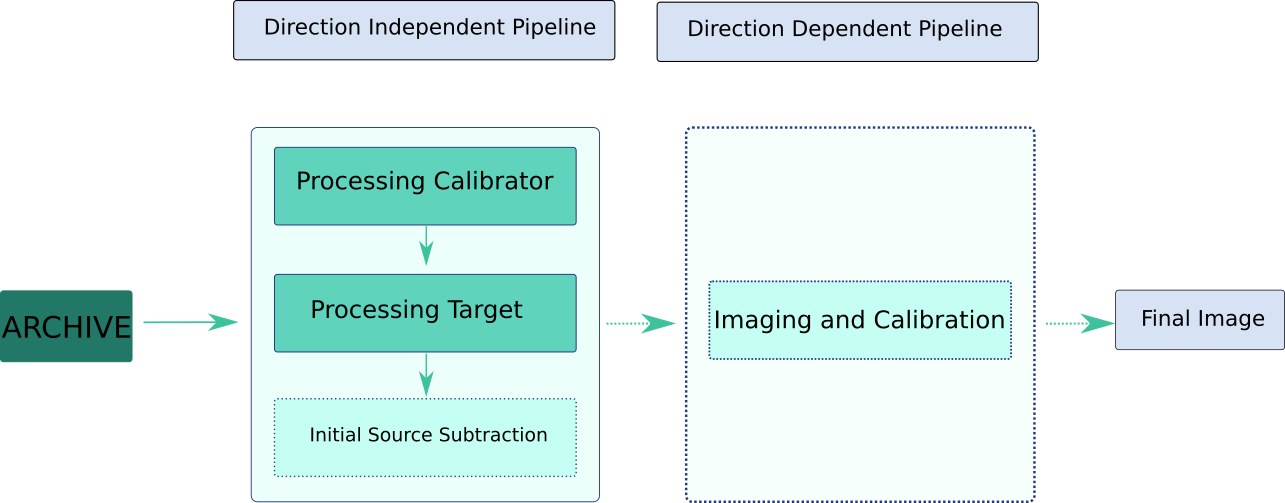
\includegraphics[width=.79\textwidth]{ch3/figures/DIDDpipe.png}\\
 \caption[Prefactor and DDFacet Data Flow]{A schematic of the data flow through the Direction Independent Pipeline (pre-FACTOR\cite{prefactor}) and one of the Direction Dependent Pipelines (DDFacet). The Initial Source Subtraction is only necessary for some DD pipelines and is not currently implemented. }
 \label{fig:ch3_both_pipes}
\end{figure}


Data reduction for the LoTSS survey is split into two pipelines: Direction Independent (DI) calibration and Direction Dependent (DD) calibration (Fig\ref{fig:ch3_both_pipes}). The Direction Independent pipeline\cite{prefactor}\cite{van2016lofar} produces images that are limited in resolution and contain instrumental effects\cite{lotss}. To achieve high fidelity continuum images, the ionospheric and beam errors must be corrected\cite{lofar_calib}. As those effects vary across the field of view, a Direction Dependent calibration step must follow. Without these corrections the image quality and resolution is severely limited\cite{van2016lofar}.  We are currently working on a GRID implementation of the Direction Dependent pipeline and will report on this in a future paper.


\subsection{Direction Independent Processing}\label{sec:ch3_dirin_process}

The LOFAR telescope consists of many antennae, each with its own electronic gain. A gain calibration needs to be performed by observing a bright calibrator source before or after the science target\cite{lofar_calib}. Using this observation, the antenna gains for the telescope are calculated. This is performed by the Calibration pipeline of the pre-FACTOR software\cite{prefactor}.  The results from this step are applied to the science target and target observation is averaged  and processed. This consists of removing Radio Frequency Interference and subtraction of bright off-axis sources, and finally calibration against a skymodel derived from surveys conducted with previous telescopes\cite{lofar_calib}\cite{van2016lofar}. These steps are performed by the Target pipeline of the pre-FACTOR software\cite{prefactor}. The result is a calibrated dataset which is up to 64 times smaller than the uncalibrated archived data.

A 16TB dataset cannot fit into a machine's memory, which is typically less than 128GB. Because of this,  the Direction Independent processing is be split by dividing the original full-bandwidth observation into independent chunks of narrower bandwidth. A typical observation spanning 48 MHz is split into 244 files called subbands each of which spans 0.1953 MHz.  These subbands are processed simultaneously, as each undergoes the same processing steps. This is a form of data-level parallelism. 

%The initial part of the LOFAR data processing can benefit from a cluster of many small machines. Doing so not only improves latency but allows for both scalability and fault tolerance, as discussed in Sections  \ref{sec:intermediate_storage} and \ref{sec:capabilities}. 

The Direction Independent calibration pipeline (Fig.\ref{fig:ch3_DIpipe}) consists of an existing set of scripts which use the LOFAR software suite\cite{lofarcookbook} to process the initial datasets. These scripts also handle the post-processing and application of the calibration results\cite{van2016lofar}. These scripts are contained in the package \emph{pre-FACTOR}\cite{prefactor}. The order of the scripts and their parameters are contained in a parameter-set file (henceforth 'parset'). The parset defines a sequence of procedures, each launching one or more executables. The execution of the procedures in a parset defines a step in the Direction Independent Pipeline. 


\subsection{Implementing the DI Calibration on the GRID}\label{sec:ch3_impl}

The LoTSS survey is mainly conducted by a team at Leiden University. The bandwidth between a University cluster and the LOFAR data archive is too low to download the data, 10 MB/s in the case of Leiden University. At Leiden University, downloading of one dataset would take 10 times longer than the processing. The processing  was moved to the SURFsara grid location at the Amsterdam Science Park\footnote{http://docs.surfsaralabs.nl/projects/grid/en/latest/Pages/Service/system\_specs.html} as there were previous successes in processing LOFAR data at SURFsara (Oonk+ in prep).  In order to take advantage of the computational resources at the SURFsara Gina cluster\cite{gina_specs}, the LOFAR pre-FACTOR pipeline was modified as part of the development LRT framework. The two steps of the DI reduction, the Calibrator and Target, were each split in two parts. The first part of the Calibrator and Target processing is parallelized by running one file per node, and the second runs combine these results. This takes advantage of the data level parallelism of LOFAR processing.

Additionally, splitting the computation makes it more robust. In the case that the download or processing of one job fails, it can be restarted without disrupting parallel jobs. When a step has finished processing, the next step can be launched automatically enabling the massive processing of LOFAR Surveys data. 

The pre-FACTOR software was designed to be run on single machines or clusters with a shared file system. Because the worker machines at the SURFsara cluster have isolated storage, scripts are included in the LOFAR Reduction Tools to load the relevant data on the worker node before processing. After a job is finished, the scripts save intermediate results to a storage location external to the cluster. 

\subsection{Data Flow and Processing Steps}\label{sec:ch3_dataflow}

A researcher interested in processing LOFAR data needs to download it from the LOFAR Long Term Archive. Leiden University leads the LoTSS survey and has a computer cluster dedicated for LOFAR processing. The connection between the Leiden location and the LOFAR data archive is typically 10 MB/s. At this rate, downloading a single 16TB LoTSS dataset completes in two weeks. At this rate, transferring 3000 datasets would take over a century. 

Unlike at Leiden University, the SURFsara clusters have a gigabit connection to the data archive, accelerating the data retrieval to 1.5 days. Additionally, having two orders of magnitude more processing nodes than at Leiden, the reduction can be further parallelized. This has accelerated the processing of one (downloaded) dataset from more than two days to less than half a day.

Using intermediate storage to hold the results from each step, the pre-FACTOR DI pipeline (Fig.\ref{fig:ch3_both_pipes}) was split into four steps as in Fig. \ref{fig:ch3_DIpipe}. The Calib 1 and Target 1 steps download the raw data at one piece per worker machine and store the processing results (Calibration Tables and Processed data respectively) in storage. The second Calibration and Target steps combine these results and process them producing the calibration solutions and datasets respectively. 


\begin{figure}
 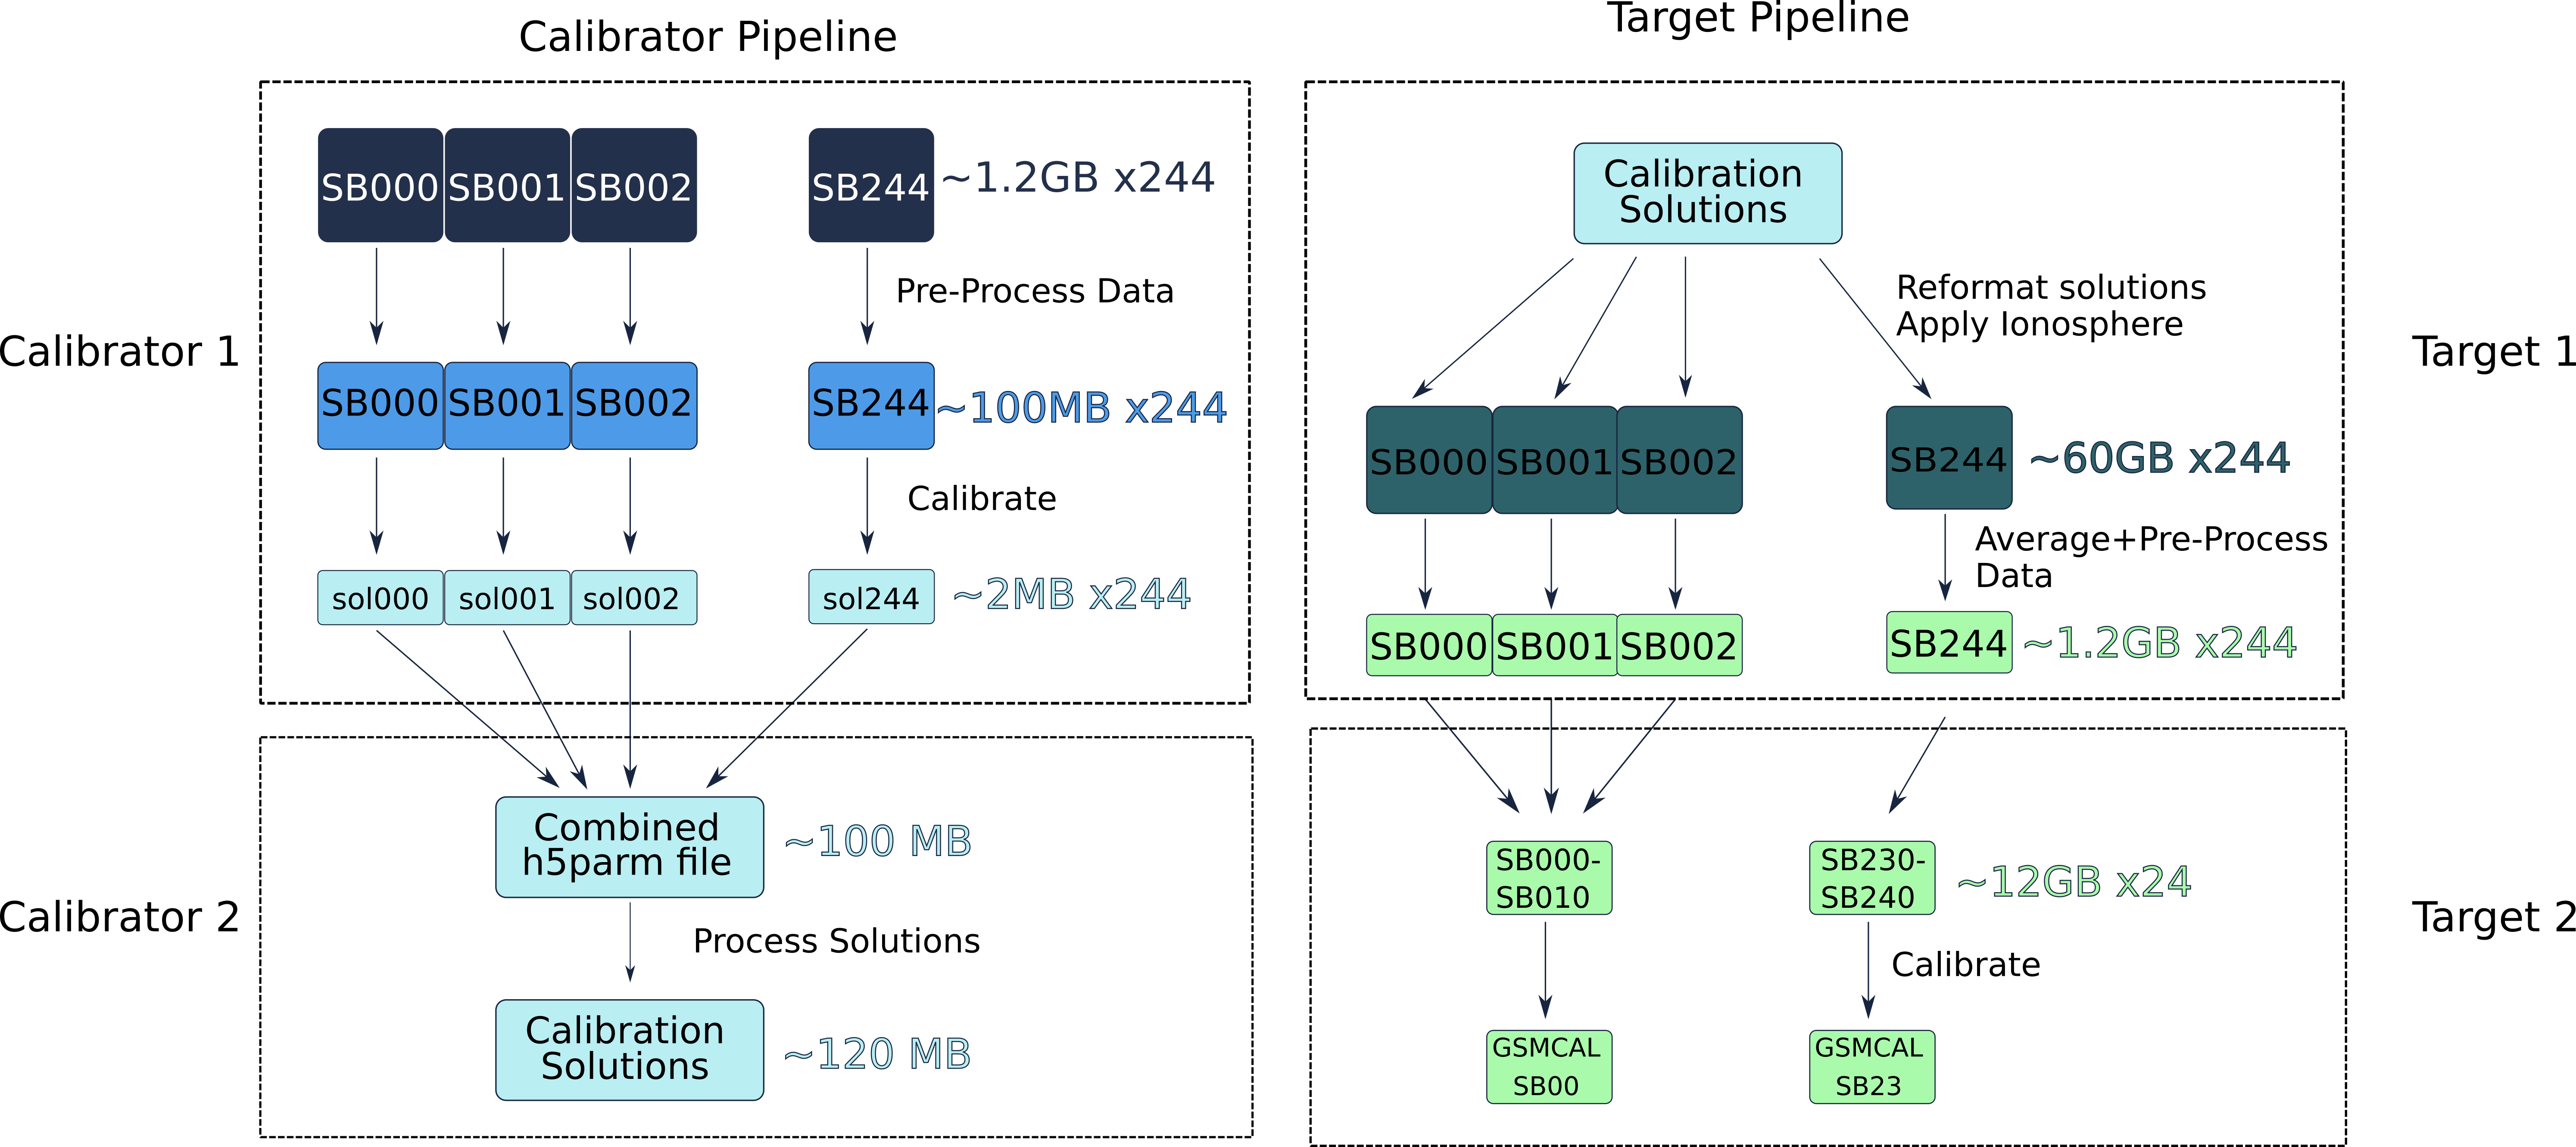
\includegraphics[width=.79\textwidth]{ch3/figures/Pipeline_parallel.png}\\
    \caption[Parallelization of prefactor processing]{Data flow and parallelization of the Direction Independent Processing. The Calibrator 1 and Target 1 steps run concurrently as independent jobs. Calibrator 2 and Target 2 combine these results. Note that the Target 1 step requires the solutions produced by the Calibrator 2 step. This places a strict ordering on the processing steps. }
 \label{fig:ch3_DIpipe}
\end{figure}



\section{Framework Design}\label{sec:ch3_design}

The LRT framework (Fig. \ref{fig:ch3_design}) was developed to automate the LOFAR Direction Independent calibration by processing the data at the Gina cluster SURFsara\cite{gina_specs}. The goal of the framework was to adapt the pre-FACTOR package to take advantage of the large computational resources and high bandwidth at this site. Thanks to the data-level parallelism, using the computational resources at the Gina cluster accelerates the data reduction. 

\begin{figure}
 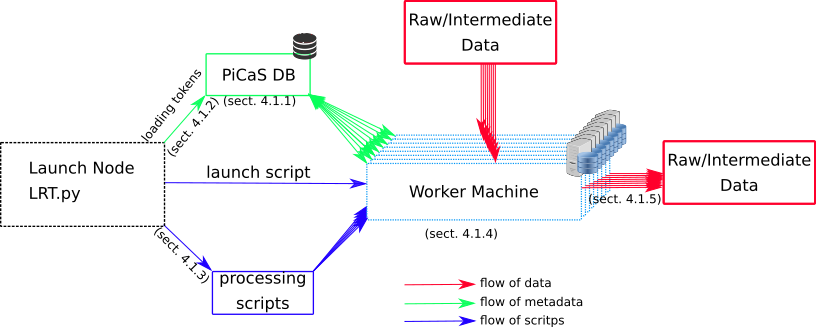
\includegraphics[width=\textwidth]{ch3/figures/design.png}\\
 \caption{Overview of the design of the LRT framework}
 \label{fig:ch3_design}
\end{figure}

\subsection{Framework Elements}
The LRT framework consists of a set of modules responsible for different parts of the data reduction. The \verb|srmlist| module handles the links to the data. If the data is on tape, it sends a command to stage it to disk. The \verb|sandbox| module creates an archive of processing scripts and uploads it to storage. The \verb|Token| module is responsible for managing metadata, which defines a processing job. Appendix \ref{sec:ch3_appendix_1} contains information on the functionality of each module and their use. 

\subsubsection{Storing Job Metadata}

The LRT framework is effective for pipelines that execute the same processing steps on a large data set split across many machines. Each part of the dataset is processed on a single machine, and the metadata of this job is stored in a remote database which can be read from and written to by the worker machine. By using a concurrent document oriented database such as CouchDB\cite{couchdb}, each document can store the metadata regarding a single processing job. This is not possible with relational databases such as MySQL.  These documents are called Tokens, as defined by the PiCaS framework\cite{picas}.

The first implementation of PiCaS and CouchDB for LOFAR data reduction was carried by J. B. R. Oonk and N. Danezi in the context of the LOFAR spectroscopy project and custom user processing (Oonk et al. in prep). This first implementation focused on processing individual data sets and required a high-level of user interaction. Here we extend this implementation to automatically handle and connect multiple runs (calibrator and target) and their products.


By logging the name of the pipeline step in the job description, each job is aware of which pipeline step it is processing and executes the appropriate scripts. Important to note is that the CouchDB documents can store text and integer values as well as file attachments. The LOFAR implementation uses attachments to store diagnostic files produced by the worker machines, lists of links to the data and parset files that define the pre-FACTOR workflow. 

\subsubsection{Creating Job Tokens}\label{sec:ch3_create_tokens}

The first step to automating batch processing is to create the job tokens which hold the processing metadata and load them into the database. In order to track multiple concurrent reductions, these tokens are combined in sets. Once this set is given a name, a batch of tokens can be created for each pipeline step and uploaded into the PiCaS server. These tokens are set in the `todo' state, indicating the processing has not yet started. The specific implementation of the `pre-FACTOR' software is discussed in Appendix \ref{sec:ch3_appendix_1}.

% \begin{figure}
%  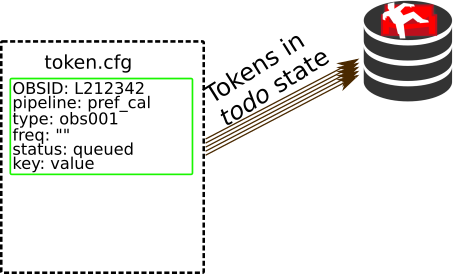
\includegraphics[width=.79\textwidth]{Token_load.png}\\
%  \caption{Loading tokens into PiCaS database (Section \ref{sec:create_tokens})}
%  \label{fig:tok_load}
% \end{figure}

\subsubsection{Packing Scripts}\label{sect:ch3_scripts}

While the PiCaS database can hold metadata which differs across jobs, pipelines or observations; the processing scripts need to be stored in a location where the worker machines have access to them. These scripts are archived and uploaded to storage and their location is added to the job token. After a worker machine locks a job token, it downloads and extracts the processing scripts, reads the metadata from the token and begins the processing (Fig.\ref{fig:ch3_tok_run}).

The location of the scripts is stored in the job token. This allows different steps of the pipeline to use different sets of scripts. The benefits from this design is that as long as the worker node has access to the URI (Universal Resource Identifier) of the scripts, it can process the data, making data reduction portable over a variety of distributed computing environments, including the GRID. This capability will be used in the future to move processing to the location of the archive (Section \ref{sec:ch3_future}). Implementation of this process is summarised in Appendix \ref{sec:ch3_appendix_1}. 


\subsubsection{Processing}

Processing is launched with a launch script executed on a worker node. This script is responsible for locking a job token, taking it from the `todo' state to the `locked' state. After the token is locked, the launch script downloads the script archive and launches the processing. For the LOFAR pre-FACTOR software, the scripts include the latest version of the pre-FACTOR repository. Additionally, there are helper scripts that set up the processing environment, download the data, post-process the output and upload the data to intermediate storage. The metadata stored in the PiCaS job token is fed into the setup and processing scripts. 

Since the processing scripts and metadata are stored remotely, the same small launch script can load many different reduction pipelines simply by changing the group of tokens it should lock.  This design choice makes it easy to create other script archives for the Direction Dependent pipeline or other LOFAR processing workflows. 

\begin{figure}
 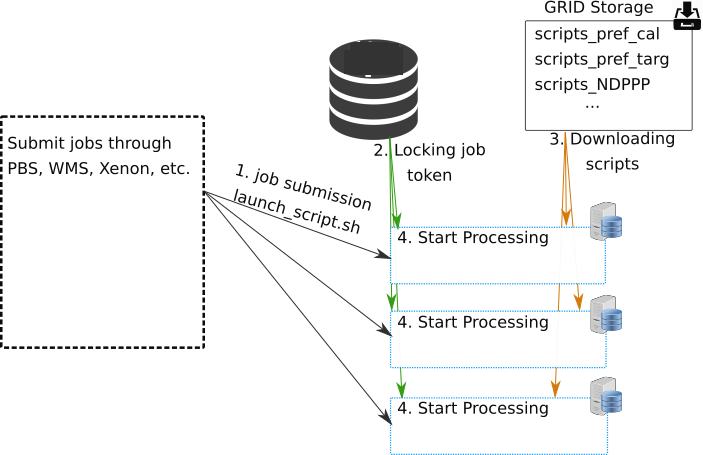
\includegraphics[width=.76\textwidth]{ch3/figures/Token_run.png}\\
    \caption[Starting processing on worker machines]{Starting processing on worker machines. Currently processing is done on SURFsara Gina nodes, however the framework has been tested at the Leiden University cluster.}
 \label{fig:ch3_tok_run}
\end{figure}


\subsubsection{Intermediate Data Storage}\label{sec:ch3_intermediate_storage}

Splitting the processing into multiple steps requires intermediate data to be stored at a location accessible to the worker machines. As the current processing is done at the Gina cluster, the intermediate results are stored in several dedicated
storage pools hosted by SURFsara. The LRT processing scripts check for the availability of an initial data set or intermediate data product on launch and download it. This avoids unnecessary repetition of reduction steps and allows to restarting a failed job.

Since the data location is static, the paths of the data are hard coded into the scripts. The framework design, however, also allows a job to log the location of its output data into the CouchDB database. Jobs in subsequent steps can read the location of their input data from the tokens of the previous job. This will be implemented when the LOFAR data processing becomes distributed across multiple locations. 

\begin{figure}
 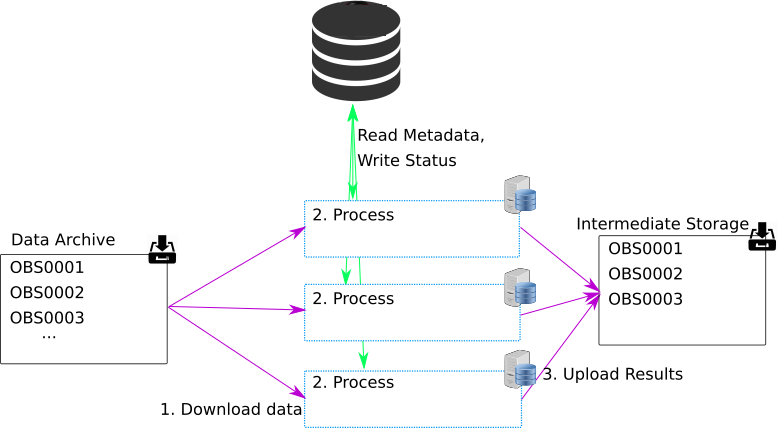
\includegraphics[width=.76\textwidth]{ch3/figures/Token_process.png}\\
    \caption[Schematic of data movement.]{Processing of LOFAR data from the Long Term Archive with results stored at an intermediate storage location.}
 \label{fig:ch3_tok_process}
\end{figure}

\subsection{LOFAR Surveys Use Case}\label{sec:ch3_use}
The LOFAR Two Meters Sky Survey requires processing of more than 8 PB of data each year in order to keep up with the data produced by the telescope. As there are more than 3000 observations planned, processing them manually is untenable. Additionally, the large raw data sizes require the data be reduced in parallel before the Direction Dependent calibration step since the data will not fit in the memory of a single machine. 

Re-purposing the LOFAR pre-FACTOR software to take advantage of the GRID computing resources by leveraging the automation provided by the LRT framework has allowed the processing of more than a hundred datasets in the timespan of four months. Additionally, this was done in the time frame that an astronomer would normally produce less than 10 Direction Independent calibrated observations, hence a providing a necessary speed up by an order of magnitude.


\subsection{Framework Capabilities}\label{sec:ch3_capabilities}

The LRT implementation is designed to be as platform independent as possible. It allows for easy extensions enabling LOFAR reduction schemes other than the LoTSS reduction. Two examples of this are the updated LOFAR GRID spectroscopy and LOFAR GRID pre-processing pipelines (Oonk+ in prep). The GRID pre-processing pipeline runs flagging of bad data and averaging, however performs no calibration. The spectroscopy pipeline uses an independent set of scripts to perform calibration,  bandwidth correction and imaging. 

Thanks to the abstraction of the metadata and scripts storage, processing is also possible at other locations. The pre-FACTOR scripts require an installation of the LOFAR software stack\cite{lofar_stack}. These requirements are met by mounting a CernVM-FS\cite{cvmfs2008}\cite{softdrive} installation of the LOFAR stack. The Cern-VM FileSystem service provides a portable pre-compiled copy of the LOFAR software.  With the CVMFS prerequisite satisfied and an active grid proxy, any computer can download data and process a job in any data reduction step. 


\subsection{Initial Results}\label{sec:ch3_performance_results}

Automatically launching jobs has made it possible to process more than 100 datasets between November 2016 and February 2017. Without a framework to automate and distribute the processing and a cluster at a Grid location, these datasets would need to be downloaded to an institute's cluster. Such standalone runs of the `pre-FACTOR' scripts typically process one observation in two weeks taking into account the data transfer time.  At the 10MB/s connection (The sustained speed at Leiden University), the downloading would take over 5 years alone. Porting the LOFAR LoTSS data reduction to a Grid location using the LRT framework has resulted in a 15x increase in data throughput. Suggestions on further increasing the throughput are presented in Section \ref{sec:ch3_future}.
 
% \subsection{Bottlenecks and Proposed Solutions}
% 
% Launching multiple processing jobs leads to large data transfer rates between the raw data archive and the processing site. While the SURFsara Grid location has a gigabit connection to the data archives, launching more than two reductions at a time results in a download bottleneck. This bottleneck is caused by the 1 Gbps public connection between LTA sites. Most of the LoTSS data is stored at the Forschungszentrum Jülich location. Thus, the 1Gbps bandwidth between the archive and processing sites limits the download to 35 hours per 16TB observation. To process the outstanding data within the five project time line, the minimum bandwidth requirement is a 2.5 Gbps uninterrupted connection to the data. Solutions to this bottleneck are presented in Section \ref{sec:future}. 


\section{Conclusion and Future Work}\label{sec:ch3_conclusion}

The goal of the LRT Framework is to create an automated software which can be used to port LOFAR processing to a massively distributed compute environment. The Direction Independent calibration of the LOFAR Two Meter Sky Survey was used as a demonstration of the capabilities of the LRT software. 

Combining the `pre-FACTOR' scripts with the LRT tools resulted in a 15x increase in throughput compared to previous data reduction strategies. Thanks to the automation provided, it is possible to process hundreds of observations, necessary for large astronomical survey projects such as the 3000+ observations of the LoTSS. 

The scalability of this framework allows to launch multiple data reductions concurrently and easily monitor their progress. The portability of the LRT framework makes it easy to move processing to archive locations, further increasing the throughput. Finally, as the framework is general, other LOFAR projects can increase throughput and automation by integrating their software. 


\subsection{Throughput Improvement}

Using the LRT framework, more than 100 datasets have passed through the Direction Independent calibration. This is more than a 15 fold increase compared to the throughput at a institution with a limited bandwidth to the data archive. From these datasets, 30 images have been produced since November 2016.  The Direction Dependent pipeline, responsible for the imaging of the DI calibrated data, is not yet automated using the LRT framework. The topic of this automation will be handled in future work. Future improvements (Section \ref{sec:ch3_future}) are expected to increase the throughput to one image per day.  

Currently, the data reduction is launched manually. There are upcoming plans to create a trigger launched by the Observatory at the end of a successful observation. Using this trigger, the processing can be integrated with the data acquisition and launched automatically at the end of the observation. Doing so enables producing an image less than a week after the observation has completed without requiring human interaction. 
% 
\subsection{Future Work}\label{sec:ch3_future}


Most of the LoTSS data is not stored at the SURFsara Grid location. Because of the high data sizes, the 1 Gbps transfer between these remote sites and SURFsara is insufficient to process the 3000+ datasets. The proposed solution is to launch the initial reduction steps (Calibrator 1 and Target 1 in Fig.\ref{fig:ch3_DIpipe}) on compute clusters at the archive locations. Running the Target 1 step at these sites will reduce the data size from 16TB to 0.5TB. The resulting intermediate data can easily be transferred over a 1 Gbps connection in 1 hour compared with the 35 hours for the original data. 

While the LRT framework successfully automated the Direction Independent calibration pipeline, it still needs to  implement the Direction Dependent processing scripts. The DI data can be easily split into pieces and processed concurrently, however current Direction Dependent pipelines cannot split the data easily. This means they will only benefit from the automation aspect of the framework. Because of this limitation of the algorithms, (Direction Dependent) processing of each dataset needs to be done on a single machine.  This part of the processing currently takes more than four days per dataset per node. To process all 3000 observations within five years, the DD reduction will need at least 8 dedicated machines continuously processing data. Nevertheless, the input data is only 200-500GB making it easier to store and transfer to institutes not part of the European Grid Infrastructure. 

The Xenon framework\cite{maasen_xenon} allows launching jobs at multiple clusters from a single location. Thanks to the portability of the LRT software, it will be possible to integrate the LOFAR reduction with Xenon. This will automate the launching of Direction Dependent processing at multiple institutions. Automatically launching these jobs will make efficient use of the computer resources at SURFsara and other sites. Using this strategy, the LoTSS project data can be processed within the anticipated timespan. 

Finally, as the reduction is automated, it can be started right after the telescope finishes the observation. Launching jobs immediately after  an observation will minimize the time staging the data from tape to disk. Currently, the staging process can take up to a week. Triggering the processing immediately after observation, an image will be produced less than a week after the data is acquired. 

Minimizing the latency between observation and science quality images will benefit the LOFAR community immensely by allowing radio astronomers to focus on their specific science case. An all-sky survey at the 150 MHz range will create a multitude of targets for follow-up with optical telescopes and result in many discoveries in the field of Radio Astronomy. A full list of science results expected from the LoTSS project can be found in\cite{lotss}. Efficient high-throughput processing of LOFAR data will empower the above science cases opening the way to  exciting new discoveries.


\begin{subappendices}

\section{Execution of LOFAR Reduction Tools }\label{sec:ch3_appendix_1}

The LRT framework handles staging of LOFAR data, packaging and uploading worker node scripts (named sandboxes), creating PiCaS job tokens and launching pilot jobs on the SURFsara Gina cluster. The framework is modular, allowing an user to execute any of the previous steps manually, or alternatively launch an automated reduction. It can be downloaded from the Github page (\href{https://github.com/apmechev/GRID_LRT}{github.com/apmechev/GRID\_LRT}) and installed with \\
\verb|python setup.py build && python setup.py install| . Documentation on the usage of the tools can be found at the Github page. 
\end{subappendices}


% \begin{thebibliography}{99}
%\bibitem{softdrive}
%Softdrive on the grid.
%\newblock Available at
%  \url{http://docs.surfsaralabs.nl/projects/grid/en/latest/Pages/Advanced/grid\_software.html\#softdrive
%  }.
%
%\bibitem{gina_specs}
%Gina specifications - grid documentation v1.0.
%\newblock Available at
%  \url{http://docs.surfsaralabs.nl/projects/grid/en/latest/Pages/Service/system\_specifications/gina\_specs.html},
%  2017.
%
%\bibitem{lofar_stack}
%Lofar software stack.
%\newblock
%  \url{http://www.lofar.org/wiki/doku.php?id=public:software\_stack\_installation},
%  2017.
%
%\bibitem{picas}
%Picas overview - grid documentation v1.0.
%\newblock
%  \url{http://doc.grid.surfsara.nl/en/latest/Pages/Practices/picas/picas\_overview.html},
%  2017.
%
%\bibitem{prefactor}
%Horneffer A.
%\newblock Prefactor: Pre-facet calibration pipeline.
%\newblock \url{https://github.com/lofar-astron/prefactor}, 2017.
%
%\bibitem{cvmfs2008}
%C~Aguado~Sanchez, J~Bloomer, P~Buncic, L~Franco, S~Klemer, and P~Mato.
%\newblock Cvmfs-a file system for the cernvm virtual appliance.
%\newblock In {\em Proceedings of XII Advanced Computing and Analysis Techniques
%  in Physics Research}, volume~1, page~52, 2008.
%
%\bibitem{couchdb}
%Chirs ANDERSON.
%\newblock Apache couchdb: The definitive guide.
%\newblock {\em http://couchdb. Apache. org/index. htm Acessado em}, 5(06):2009,
%  2009.
%
%\bibitem{ska_cloud_memo}
%Domingos Barbosa, Jo{\~a}o~Paulo Barraca, Dalmiro Maia, Bruno Carvalho, Jorge
%  Vieira, Paul Swart, Gerhard Le~Roux, Swaminathan Natarajan, Arnold van
%  Ardenne, and Luis Seca.
%\newblock Power monitoring and control for large scale projects: Ska, a case
%  study.
%\newblock In {\em SPIE Astronomical Telescopes+ Instrumentation}, pages
%  99100L--99100L. International Society for Optics and Photonics, 2016.
%
%\bibitem{simcity}
%Joris Borgdorff, Harsha Krishna, and Michael~H Lees.
%\newblock Sim-city: An e-science framework for urban assisted decision support.
%\newblock {\em Procedia Computer Science}, 51:2327--2336, 2015.
%
%\bibitem{picas_git}
%Jan Bot.
%\newblock Picas: Python client using couchdb as a token pool server.
%\newblock \url{https://github.com/jjbot/picasclient}, 2017.
%
%\bibitem{clemencic2014new}
%Marco Clemencic and B~Couturier.
%\newblock A new nightly build system for lhcb.
%\newblock In {\em Journal of Physics: Conference Series}, volume 513, page
%  052007. IOP Publishing, 2014.
%
%\bibitem{lofar_data}
%Hanno Holties, Adriaan Renting, and Yan Grange.
%\newblock The lofar long-term archive: e-infrastructure on petabyte scale.
%\newblock In {\em SPIE Astronomical Telescopes+ Instrumentation}, pages
%  845117--845117. International Society for Optics and Photonics, 2012.
%
%\bibitem{cvmfsatlas}
%Grigory Rybkin.
%\newblock Atlas software packaging.
%\newblock In {\em Journal of Physics: Conference Series}, volume 396, page
%  052063. IOP Publishing, 2012.
%
%\bibitem{li2017reliability}
%Y~Li.
%\newblock Reliability of long heterogeneous slopes in 3d: Model performance and
%  conditional simulation.
%\newblock 2017.
%
%\bibitem{maasen_xenon}
%Jason Maassen, Stefan Verhoeven, Joris Borgdorff, Niels Drost, cwmeijer,
%  Jurriaan~H. Spaaks, Rob~V. van Nieuwpoort, Piter~T. de~Boer, and Ben van
%  Werkhoven.
%\newblock Xenon: Xenon 1.1.0, December 2015.
%
%\bibitem{lofarcookbook}
%RF~Pizzo et~al.
%\newblock The lofar imaging cookbook v2.0.
%\newblock {\em internal ASTRON report}, 2010.
%
%\bibitem{sante2010development}
%Tom SANTE.
%\newblock Development of (graphical) web applications for the processing and
%  interpretation of arraycgh data.
%\newblock 2010.
%
%\bibitem{lotss}
%TW~Shimwell, HJA R{\"o}ttgering, PN~Best, WL~Williams, TJ~Dijkema,
%  F~de~Gasperin, and MJ~Hardcastle.
%\newblock The lofar two-metre sky survey. i. survey description and preliminary
%  data relase.
%\newblock {\em Astronomy \& Astrophysics}, 2016.
%
%\bibitem{lofar_calib}
%Cyril Tasse, Ger van Diepen, Sebastiaan van~der Tol, Reinout~J van Weeren,
%  Joris~E van Zwieten, Fabien Batejat, Sanjay Bhatnagar, Ilse van Bemmel, Laura
%  B{\^\i}rzan, Annalisa Bonafede, et~al.
%\newblock Lofar calibration and wide-field imaging.
%\newblock {\em Comptes Rendus Physique}, 13(1):28--32, 2012.
%
%\bibitem{van2013lofar}
%MP~Van~Haarlem, MW~Wise, AW~Gunst, George Heald, JP~McKean, JWT Hessels,
%  AG~De~Bruyn, Ronald Nijboer, John Swinbank, Richard Fallows, et~al.
%\newblock Lofar: The low-frequency array.
%\newblock {\em Astronomy \& Astrophysics}, 556:A2, 2013.
%
%\bibitem{van2016lofar}
%RJ~Van~Weeren, WL~Williams, MJ~Hardcastle, TW~Shimwell, DA~Rafferty, J~Sabater,
%  G~Heald, SS~Sridhar, TJ~Dijkema, G~Brunetti, et~al.
%\newblock Lofar facet calibration.
%\newblock {\em The Astrophysical Journal Supplement Series}, 223(1):2, 2016.
%
%\bibitem{bioinfo}
%Anjani Ragothaman, Sairam~Chowdary Boddu, Nayong Kim, Wei Feinstein, Michal
%  Brylinski, Shantenu Jha, and Joohyun Kim.
%\newblock Developing ethread pipeline using saga-pilot abstraction for
%  large-scale structural bioinformatics.
%\newblock {\em BioMed research international}, 2014, 2014.
%
%\bibitem{ecoinfo}
%William~K Michener and Matthew~B Jones.
%\newblock Ecoinformatics: supporting ecology as a data-intensive science.
%\newblock {\em Trends in ecology \& evolution}, 27(2):85--93, 2012.
%
%\bibitem{swift}
%Yong Zhao, Mihael Hategan, Ben Clifford, Ian Foster, Gregor Von~Laszewski,
%  Veronika Nefedova, Ioan Raicu, Tiberiu Stef-Praun, and Michael Wilde.
%\newblock Swift: Fast, reliable, loosely coupled parallel computation.
%\newblock In {\em Services, 2007 IEEE Congress on}, pages 199--206. IEEE, 2007.
%
%\bibitem{scalable}
%Shayan Shams, Nayong Kim, Xiandong Meng, Ming~Tai Ha, Shantenu Jha, Zhong Wang,
%  and Joohyun Kim.
%\newblock A scalable pipeline for transcriptome profiling tasks with on-demand
%  computing clouds.
%\newblock In {\em Parallel and Distributed Processing Symposium Workshops, 2016
%  IEEE International}, pages 443--452. IEEE, 2016.
%
%\bibitem{aperturesynth}
%WN~Brouw.
%\newblock Aperture synthesis.
%\newblock In {\em Image Processing Techniques in Astronomy}, pages 301--307.
%  Springer, 1975.
%
%\bibitem{neurogrid}
%JD~Van~Horn, J~Dobson, J~Woodward, M~Wilde, Y~Zhao, J~Voeckler, and I~Foster.
%\newblock Grid-based computing and the future of neuroscience computation,
%  methods in mind, 2005.
%  
%\bibitem{cvmfsnova}
%GS~Davies, JP~Davies, Brian Rebel, Kanika Sachdev, Jan Zirnstein, C~Group,
%  et~al.
%\newblock Software management for the no$\nu$aexperiment.
%\newblock In {\em Journal of Physics: Conference Series}, volume 664, page
%  062011. IOP Publishing, 2015.
%
%\bibitem{pegasus}
%Ewa Deelman, Gurmeet Singh, Mei-Hui Su, James Blythe, Yolanda Gil, Carl
%  Kesselman, Gaurang Mehta, Karan Vahi, G~Bruce Berriman, John Good, et~al.
%\newblock Pegasus: A framework for mapping complex scientific workflows onto
%  distributed systems.
%\newblock {\em Scientific Programming}, 13(3):219--237, 2005.
%
%\end{thebibliography}
%
% \end{document}

%%%% This is file `elsarticle-template-1-num.tex',
%%%%
%%%% Copyright 2009 Elsevier Ltd
%%%%
%%%% This file is part of the 'Elsarticle Bundle'.
%%%% ---------------------------------------------
%%%%
%%%% It may be distributed under the conditions of the LaTeX Project Public
%%%% License, either version 1.2 of this license or (at your option) any
%%%% later version.  The latest version of this license is in
%%%%    http://www.latex-project.org/lppl.txt
%%%% and version 1.2 or later is part of all distributions of LaTeX
%%%% version 1999/12/01 or later.
%%%%
%%%% Template article for Elsevier's document class `elsarticle'
%%%% with numbered style bibliographic references
%%%%
%%%% $Id: elsarticle-template-1-num.tex 149 2009-10-08 05:01:15Z rishi $
%%%% $URL: http://lenova.river-valley.com/svn/elsbst/trunk/elsarticle-template-1-num.tex $
%%%%
%%\documentclass[preprint,5p]{elsarticle}
%%
%%%% Use the option review to obtain double line spacing
%%%% \documentclass[preprint,review,12pt]{elsarticle}
%%
%%%% Use the options 1p,twocolumn; 3p; 3p,twocolumn; 5p; or 5p,twocolumn
%%%% for a journal layout:
%%%% \documentclass[final,1p,times]{elsarticle}
%%%% \documentclass[final,1p,times,twocolumn]{elsarticle}
%%%% \documentclass[final,3p,times]{elsarticle}
%%%% \documentclass[final,3p,times,twocolumn]{elsarticle}
%%%% \documentclass[final,5p,times]{elsarticle}
%%%% \documentclass[final,5p,times,twocolumn]{elsarticle}
%%\usepackage{natbib}
%%\bibliographystyle{abbrvnat}
%%\setcitestyle{authoryear,open={(},close={)}} %Citations bracketed with ()
%%\setcitestyle{citesep={;}} %Makes multiple citations with ;
%%%% The graphicx package provides the includegraphics command.
%%\usepackage{graphicx}
%%\usepackage{footnote}
%%\usepackage{epsfig}
%%
%%\makesavenoteenv{tabular}
%%\makesavenoteenv{table}
%%
%%
%%\usepackage{url}
%%%% The amssymb package provides various useful mathematical symbols
%%\usepackage{amssymb}
%%%% The amsthm package provides extended theorem environments
%%%% \usepackage{amsthm}
%%
%%\usepackage{dcolumn}% Align table columns on decimal point
%%\usepackage{bm}% bold math
%%%% The lineno packages adds line numbers. Start line numbering with
%%%% \begin{linenumbers}, end it with \end{linenumbers}. Or switch it on
%%%% for the whole article with \linenumbers after \end{frontmatter}.
%%\usepackage[switch]{lineno}
%%%\linenumbers
%%
%%\usepackage{caption}
%%\usepackage{subcaption}
%%%% natbib.sty is loaded by default. However, natbib options can be
%%%% provided with \biboptions{...} command. Following options are
%%%% valid:
%%
%%%%   square -  square brackets are used   [option]
%%%%   curly  -  curly braces are used      {option}
%%%%   angle  -  angle brackets are used    <option>
%%%%   semicolon  -  multiple citations separated by semi-colon
%%%%   colon  - same as semicolon, an earlier confusion
%%%%   comma  -  separated by comma
%%%%   numbers-  selects numerical citations
%%%%   super  -  numerical citations as superscripts
%%%%   sort   -  sorts multiple citations according to order in ref. list
%%%%   sort&compress   -  like sort, but also compresses numerical citations
%%%%   compress - compresses without sorting
%%%%
%%%% \biboptions{comma,round}
%%
%%% \biboptions{}
%%\journal{Astronomy and Computing}
%%
%%% % 
%%\begin{document}\sloppy
%%
%%\begin{frontmatter}
%%
%%%% Title, authors and addresses

%\addcontentsline{toc}{chapter}{Pipeline Collector}

\chapter[Pipeline Collector]{\textit{Pipeline Collector}: Gathering performance data for distributed astronomical pipelines}\label{ch:pipeline_collector}
\setcounter{footnote}{0}

%peedup real life pipelines performance automatic measurements radio astronomy
%\thanks{A footnote to the article title}%X
\author{Alexandar P. Mechev$^a$ }
%\ead{apmechev@strw.leidenuniv.nl}

% \altaffiliation[Also at ]{Physics Department, XYZ University.}%Lines break automatically or can be forced with \\
\author{Aske Plaat$^b$}%
\author{J.B. Raymond Oonk$^a$$^,$$^c$}%
\author{Huib T. Intema$^a$}%
\author{Huub J.A. R\"ottgering$^a$}%

\date{\today}% It is always \today, today,
%\address{$^a$Leiden Observatory, Niels Bohrweg 2, 2333 CA Leiden, the Netherlands}
%\address{$^b$Leiden Institute of Advanced Computer Science, Niels Bohrweg 1, 2333 CA Leiden, the Netherlands}
%\address{$^c$ASTRON,  Oude Hoogeveensedijk 4, 7991 PD Dwingeloo, the Netherlands}

\begin{abstract}
Modern astronomical data processing requires complex software pipelines to process ever growing data sets. For radio astronomy, these pipelines have become so large that they need to be distributed across a computational cluster. This makes it difficult to monitor the performance of each pipeline step. To gain insight into the performance of each  step, a performance monitoring utility needs to be integrated with the pipeline execution. In this work we have developed such a utility and integrated it with the calibration pipeline of the Low Frequency Array, LOFAR, a leading radio telescope. We tested the tool by running the pipeline on several different compute platforms and collected the performance data. Based on this data, we make well informed recommendations on future hardware and software upgrades. The aim of these upgrades is to accelerate the slowest processing steps for this LOFAR pipeline. The \textit{pipeline\_collector} suite is open source and will be incorporated in future LOFAR pipelines to create a performance database for all LOFAR processing. 
% \begin{description}

% \item[Prefactor]
% The \texttt{LOFAR} pre-factor pipeline prepares LOFAR Observations for creating high fidelity images. 
% \end{description}
\end{abstract}

%\begin{keyword}
%Radio Astronomy \sep Performance Analysis \sep Profiling \sep High Performance Computing
%\end{keyword}

%\end{frontmatter}

%\maketitle\makesavenoteenv{tabular}

%
%\tableofcontents
%\linenumbers

\section{\label{sec:ch4_intro}Introduction }
\setcounter{footnote}{0}

Astronomical data often requires significant processing before it is considered ready for scientific analysis. This processing is done increasingly by complex and autonomous software pipelines, often consisting of numerous processing steps, which are run without user interaction. It is necessary to collect performance statistics for each pipeline step. Doing so will enable scientists to discover and address software and hardware inefficiencies and produce scientific data at a higher rate. To identify these inefficiencies, we have extended the performance monitoring package \textit{tcollector}\footnote{https://github.com/OpenTSDB/tcollector}\citep{tcollector}. The resulting suite, \textit{pipeline\_collector}, makes it possible to use \textit{tcollector} to record data for complex pipelines. We have used a leading radio telescope as the test case for the \textit{pipeline\_collector} suite. The discoveries made with our software will help remove bottlenecks and suggest hardware requirements for current and future processing clusters. We summarize our findings in Table \ref{table:ch4_results} in Section \ref{sec:ch4_results}.

Over the past two decades, processing data in radio astronomy has increasingly moved from personal machines to large compute clusters. Over this time, radio telescopes have undergone upgrades in the form of wide band receivers and upgraded correlators \citep{lofarcobalt,gmrt_upgrade}. In addition, several aperture synthesis arrays such as the Low Frequency Array \citep[LOFAR,][]{LOFAR}, Murchison Widefield Array \citep[MWA][]{MWA,mwa2} and MeerKAT \citep{meerkat} have begun observing the radio sky, leading to an increase of data rates by up to 3 orders of magnitude \citep{mwa_data_size,meerkat_size}.

As the data acquisition rate has increased, data size has entered the Petabyte regime, and processing requirements increased to millions of CPU-hours. In order for processing to match the acquisition rate, the data is increasingly processed at large clusters with high-bandwidth connections to the data. An important case where data processing is done at a high throughput cluster is the LOFAR radio telescope.

The LOFAR telescope is a European low frequency aperture synthesis radio telescope centered in the Netherlands with stations stretching across Europe. This aperture synthesis telescope requires significant data processing before producing scientific images \citep{lofar_prefactor,Wendy_bootes,tassesmirnov,oonk_2014}. In this work, we will use our performance monitoring utility, \textit{pipeline\_collector}\footnote{https://gitlab.com/apmechev/pipeline\_collector.git}, to study the first half of the LOFAR processing, the Direction Independent (hereafter  DI) pipeline. 

One major project for the LOFAR telescope is the Surveys Key Science Project (SKSP) \citep{lotss}. This project consists of more than 3000 observations of 8 hours each, 600 of which have been observed. These observations need to be processed by a DI pipeline, the results of which are calibrated by a Direction Dependent (DD) pipeline. The DI pipeline is implemented in the software package \textit{prefactor}\footnote{available at \protect\url{https://github.com/lofar-astron/prefactor}}. The \textit{prefactor} pipeline is itself split into four stages and implemented at the SURFsara Grid location at the Amsterdam e-Science centre \citep{SurfSara,mechev17}. The automation and simple parallelization has decreased the run time per data set from several days to six hours, making it comparable to the observation rate. To better understand and optimize the performance of the \textit{prefactor} pipeline, we require detailed performance information for all steps of the processing software. We have developed a utility to gather this information for data processing pipelines running on distributed compute systems. 

In this work, we will use the \textit{pipeline\_collector} utility to study the LOFAR \textit{prefactor} pipeline and suggest optimization based on our results. To test the software on a diverse set of hardware, we will set up the monitoring package on four different computers and collect data on the pipeline's performance. Using this data, we discuss several aspects of the LOFAR software which we present in Table \ref{table:ch4_results}. Finally we discuss the broader context of these optimizations in relation to the LOFAR SKSP project and touch on the integration of \textit{pipeline\_collector} with the second half of the data processing pipeline, the DD calibration and imaging. 
    
 \begin{table*}[!htb]
 \begin{center}
  \begin{tabular}{ l | p{130mm} }
    \hline
    Result \# & Description  \\ \hline
    \hline
    \textbf{R1} & Native compilation of the software performs comparably to pre-compiled binaries on two test machines. \\ \hline
    \textbf{R2} &  The processing steps do not appear to accelerate significantly on a faster processor or with larger cache size. \\ \hline
    \textbf{R3} & Both calibration steps (\textit{calib\_cal} and \textit{gsmcal\_solve}) show linear correlation between speedup and memory bandwidth. \\ \hline
    \textbf{R4} &  Disk read/write speed does not affect the completion time of the slowest steps. \\ \hline
    \textbf{R5} & Both calibration steps do not use large amounts of RAM despite processing data on the order of Gigabytes. \\ \hline
    \textbf{R6} & The \textit{calib\_cal} step can suffer up to 20\% of Level 1 Instruction Cache misses, while gsmcal only has 5\% of these misses. \\ \hline
    \textbf{R7} & Both calibration steps are impacted by Level 2 Cache eviction at comparable rates. \\ \hline
    \textbf{R8} & The \textit{calib\_cal} step stalls on resources 70\% of cycles while the gsmcal step only 30\% of them. \\ \hline
    \textbf{R9} & The \textit{calib\_cal} uses the CPU at full efficiency for only 10 \% of the CPU cycles. \\ \hline
    \hline
  \end{tabular}   
  \caption{A table of all the results presented in Section \ref{sec:ch4_results}.}
  \label{table:ch4_results}
   \end{center}
 \end{table*}
 
 
\subsection{Related Work}\label{sec:ch4_related}

Scientific fields that need to process large data sets employ some type of data processing pipelines.  Such pipelines include e.g. solar imaging \citep{solar_pipeline}, neuroscience imaging \citep{optimize_pipeline} and infrared astronomy \citep{herschel}. While these pipelines often log the start and finishing times of each step (using tools such as pegasus-kickstart \citep{kickstart}), they do not collect detailed time series performance data throughout the run. 

At a typical compute cluster the performance of every node in a distributed systems is monitored using utilities, such as Ganglia \citep{ganglia}. These tools only monitor the global system performance. 
If one is interested in specific processes, then the Linux procfs \citep{procfs} is used. The procfs system can be used to analyze the performance of individual pipeline steps. Likewise, the Performance API \citep[PAPI,][]{papi} is a tool which collects detailed low level information on the CPU usage per process. Collecting detailed statistics at the process level is required to understand and optimize the performance of the LOFAR pipeline and we will integrate PAPI into \textit{pipeline\_collector} in the future. Finally, DTrace\citep{dtrace} is a Sun Microsystems tool which makes it possible to write profiling scripts that access data from the kernel and can be used to monitor process or system performance at run time with minimal overhead. As DTrace was not installed on either of the processing clusters, we have not used it to monitor the pipeline's performance. 

The Linux procfs system and PAPI record data which is already made available by the Linux kernel. This option incurs insignificant overhead as it uses data the kernel and processor already log. Likewise PAPI reads performance counters that the CPU automatically increments during processing. These profiling utilities can run concurrently with the scientific payload without using more than 1-2\% of system resources. Their low overhead is why we choose to use them to collect performance data. 

Other tools for performance analysis such as Valgrind \citep{valgrind} collect very detailed performance information. This comes at the expense of execution time: running with Valgrind, the processing time slows by up to two orders of magnitude. As such, we do not use Valgrind along the LOFAR software. 

\section[Measuring LOFAR Pipeline performance with pipeline\_collector]{Measuring LOFAR Pipeline performance with \\pipeline\_collector}\label{sec:ch4_methods}
We developed the package \textit{pipeline\_collector} as an extension of  the performance collection package \textit{tcollector}. \textit{pipeline\_collector} makes it possible to collect performance data for complex multi-step pipelines. Additionally, it makes it easy to record performance data from other utilities. A performance monitoring utility that we plan to integrate in the future are the PAPI tools described in section \ref{sec:ch4_related}. The resulting performance data was recorded in a database and analyzed. For our tests, we used the LOFAR \textit{prefactor} pipeline, however with minor modifications, any multi-step pipeline can be profiled. 

\textit{tcollector} is a software package that automatically launches 'collector' scripts. These scripts are  sample the specific system resource and send the data to the main tcollector process. This process then sends the data to the dedicated time series database. We created custom scripts to monitor processes launched by the \textit{prefactor} pipeline (\ref{sec:ch4_customcollectors}). 

In this work, we use a sample LOFAR SKSP data set as a test case. A particular focus was to understand the effect of hardware on the bottlenecks of the LOFAR data reduction. To gain insight into the effect of hardware on \textit{prefactor} performance, the data was processed on four different hardware configurations (Table \ref{tab:ch4_nodes}). As typical upgrade cycle for cluster hardware is five years, our results will be used to select optimal hardware for future clusters tasked with LOFAR processing.  

\subsection{\textit{Prefactor} Pipeline}

The LOFAR \textit{prefactor} pipeline \citep{lofar_prefactor} is a software pipeline that performs direction independent calibration using the LOFAR software. The LOFAR software stack is a software package containing commonly used processing software used by LOFAR pipelines \citep{cookbook,lofar_NDPPP}. These tools are built and maintained by ASTRON\footnote{ASTRON: Netherlands Institute for Radio Astronomy, url{https://www.astron.nl/}}. 

The \textit{prefactor} pipeline performs a sequence of four stages, namely the calibrator and target calibration. The first half of \textit{prefactor} processes data from a calibration source and the second half processes a science target. Altogether, this processing takes six hours on a high-throughput cluster. The final result is a data-set ready for creating  images of the sky at radio wavelengths. Figure \ref{fig:ch4_four_steps_box} shows a graphical view of the prefactor pipeline's Calibrator and Target stages.


The Calibrator stage consists of the \textit{ndppp\_prep\_cal} and the \textit{calib\_cal} step. The former flags radio interference and averages the data, and the latter performs gain calibration on a bright calibration source. It is followed by the \textit{fitclock} step which fits a clock-TEC model to the calibration solutions \citep{lofar_prefactor}.  

The Target stage consists of a \textit{ndppp\_prep\_targ} step, \textit{predict\_ateam}, \textit{gsmcal\_solve} and \textit{gsmcal\_apply} steps. The first two of these steps flag and average the target data and calculate contamination by bright off-axis radio sources. The \textit{gsmcal\_solve} step determines phase solutions for each antenna using a model of the target and the results of the \textit{ndppp\_prep\_targ} step. Finally, the \textit{gsmcal\_apply} step applies these solutions to the target data. Figure \ref{fig:ch4_4_steps_pies} shows the percentage of time spent by these steps for the four \textit{prefactor} stages.

\begin{figure}[H]
    \centering
    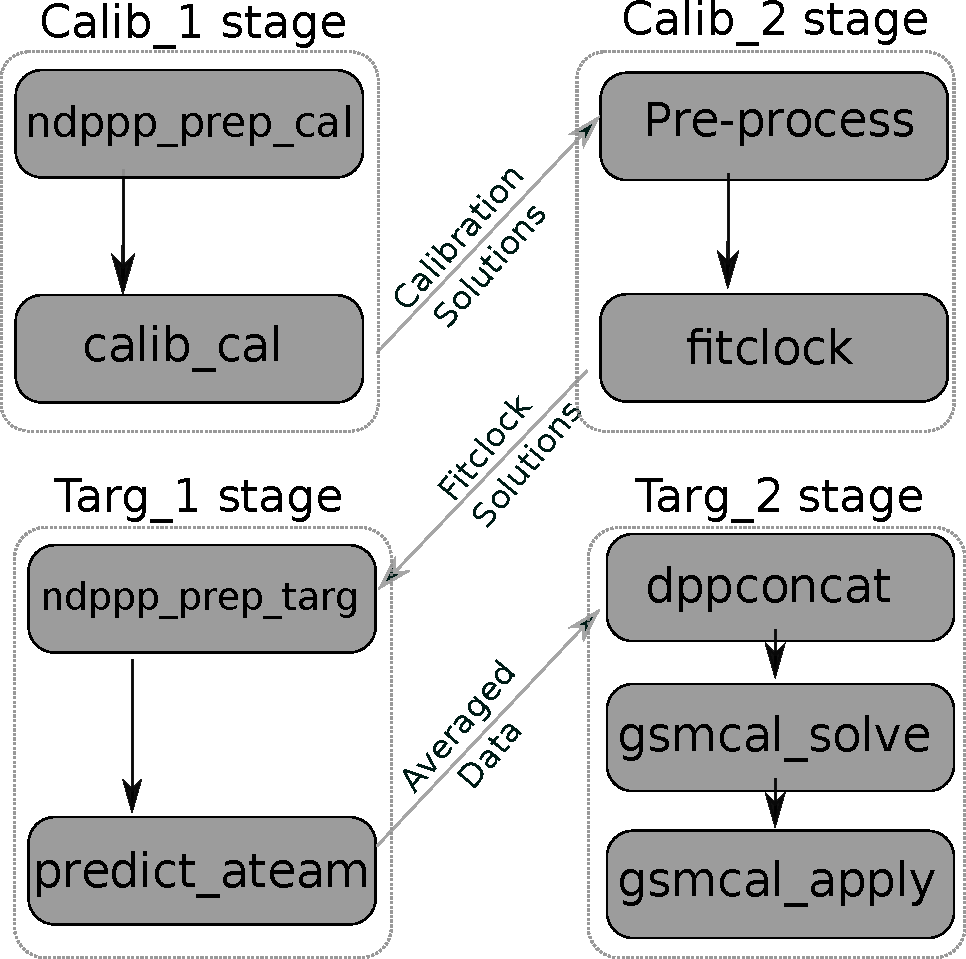
\includegraphics[width=0.5\linewidth]{ch4/figures/fig1/fig1.pdf}
      \caption[The four processing stages that make up the prefactor pipeline.]{The four processing stages that make up the prefactor pipeline. The Calibrator stages (top) process a known bright calibrator to obtain the gain for the LOFAR antennas. The Target stages (bottom) process the scientific observation to remove Direction Independent effects. The \textit{pref\_cal1} and \textit{pref\_targ1} stages are massively parallelized across nodes without the need of an interconnect. The \textit{pref\_cal2} step runs only on one node, while \textit{pref\_targ2} is parallelized on 25 nodes. As the LOFAR software does not use MPI, we can run each processing job in isolation. }
	\label{fig:ch4_four_steps_box}
\end{figure}

\begin{figure}[H]
    \centering
    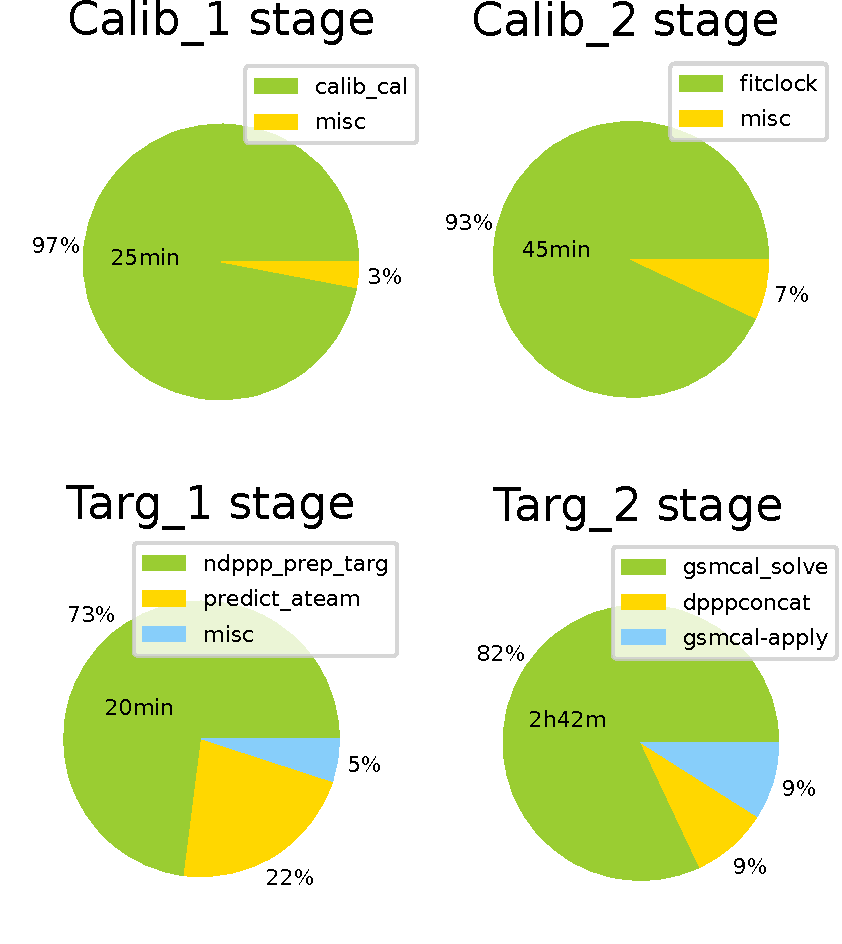
\includegraphics[width=0.5\linewidth]{ch4/figures/fig2/4pies.pdf}
      \caption[Portion of processing time taken by each step for the four prefactor stages.]{Portion of processing time taken by each step for the four prefactor stages, as reported by the Prefactor software. For each stage, the majority of processing time is spent during one or two steps. This is due to the fact that each prefactor stage also has intermediate book-keeping steps explicitly included in the pipeline. For each pipeline stage, the mean processing time for the longest running steps at SURFsara is also indicated. It should be noted that while faster, pref\_cal1 runs 10 times as many jobs as pref\_targ2. }
	\label{fig:ch4_4_steps_pies}
\end{figure}

 %\footnotetext[4]{\textit{calib\_cal} and \textit{gsmcal\_solve}}

\subsection{Performance suite}
Cluster performance is frequently monitored using utilities such as Ganglia \citep[][discussed in Section \ref{sec:ch4_related}]{ganglia}. These tools cannot access individual processes and thus cannot collect data on a per-process basis. To collect such data, each process launched by the active pipeline step needs to be profiled individually. Our utility is designed to gather such performance data.

Our monitoring package, \textit{pipeline\_collector} adds custom performance collectors (\ref{sec:ch4_customcollectors}) to the performance collection framework \textit{tcollector}. We use these collectors to monitor individual pipeline steps as defined by the user\footnote{https://gitlab.com/apmechev/pipeline\_collector.git}. The tools attach to processes launched by the pipeline and record performance data at a one second interval. This sampling frequency is at high enough resolution to detect trends and anomalies in hardware utilization, and still result in a reasonable database size. The performance data is uploaded to a remote time series database, OpenTSDB \citep{opentsdbsite}. Details on the data collection can be found in  \ref{sec:ch4_appendix1}.

\subsubsection{Performance API}\label{sec:ch4_papi2}

The time-series database is also used to collect low-level CPU information for each process. This information is collected by the PAPI interface (discussed in Section \ref{sec:ch4_related}). This was done through the papiex utility\footnote
{Available at https://bitbucket.org/minimalmetrics/papiex-oss} \citep{papiex}. This utility records the CPU's internal performance counters. A CPU's performance counters record information on how efficiently the software uses the CPU's resources. The results from this test are detailed in Section \ref{sec:ch4_PAPI}.

\subsection{Test Hardware}

In order to study the effect of different hardware configurations on the performance of LOFAR processing, the \textit{prefactor} pipeline was run on four different sets of hardware. The four machines tasked with processing LOFAR data comprised nodes at three computational clusters and a personal computer. The tests were run while the systems were idle to make sure there is no interference of other software with the LOFAR processing. Table \ref{tab:ch4_nodes} details the specifics of the four test machines.

 \begin{table}
     \begin{center} 
\resizebox{\textwidth}{!}{
  \begin{tabular}{ l | c | c | c | c | c | c }
    \hline
    Location & CPU Speed (MHz) & CPU Model & Micro-architecture & Cache Size & RAM Speed\footnotemark & Disk Speed\footnotemark \\ \hline
    \hline
    Leiden & 2200 & E5-4620 & Sandy Bridge & 16 MB  & 1.4 GB/s & 99.7 MB/s \\ \hline
    SURFsara & 2500 & E5-2680 & Sandy Bridge & 30 MB  & 2.5 GB/s & 65.4 MB/s \\ \hline
    Hatfield &  2900 & E5-2660 & Sandy Bridge  & 20 MB   & 2.4 GB/s & 155 MB/s\\ \hline
    Laptop & 3300 & E3-1505M & Skylake &  8 MB  & 4.7 GB/s & 822 MB/s\\ \hline
    \hline
  \end{tabular}   
  \label{tab:ch4_nodes}}
         \caption[Hardware specifications of the four test machines.]{CPU, Cache, RAM and Storage specifications of the four test machines. The tested machines span a factor of 1.5x in CPU speed, 4x in cache and RAM Speed and $~$10x in Disk speed.}
  \end{center}
 \end{table}




\section{LOFAR Prefactor Test Case}\label{sec:ch4_results}
  
With the test set described in Section \ref{sec:ch4_methods}, we aim to understand processing bottlenecks in the \textit{prefactor} pipeline and make informed decisions on future hardware and software upgrades. To do so, we processed a sample observation at institutes that typically process LOFAR data. 

From the data collected by processing the sample observation, we determined the slowest pipeline steps. These steps were the \textit{calib\_cal} and \textit{gsmcal\_solve}, seen in Figure \ref{fig:ch4_4_steps_pies}. The \textit{calib\_cal} step is implemented by the software \texttt{bbs-reducer} \citep{cookbook,bbs_selfcal} and the \textit{gsmcal\_solve} step is implemented by \texttt{NDPPP} \citep{cookbook,lofar_NDPPP}. Both \texttt{bbs-reducer} and \texttt{NDPPP} are part of the LOFAR software suite.

We collected performance statistics using the \textit{pipeline\_collector} suite as discussed in Section \ref{sec:ch4_methods}. The run time of the slowest \textit{prefactor} steps on the four machines is shown in figure \ref{fig:ch4_calibcal_fitclock_bars}. The results discovered using \textit{pipeline\_collector} are listed in Table \ref{table:ch4_results} and discussed in Section \ref{sec:ch4_res_tcoll}. Using the PAPI interface (discussed in Section \ref{sec:ch4_papi2}) CPU performance data was collected. The results from this test are detailed in Section \ref{sec:ch4_PAPI}.


 
We will present a number of insights into the performance of the LOFAR software collected by the profiling suite. The results are presented in Table \ref{table:ch4_results} and are grouped in three main areas. The effect of compilation on the run time was result \textbf{R1}. The set of results \textbf{R2}, \textbf{R3}, \textbf{R4} and \textbf{R5} were obtained using the \textit{pipeline\_collector} package. Results  \textbf{R6}, \textbf{R7}, \textbf{R8} and \textbf{R9} were collected with the PAPI package, which will be integrated into \textit{pipeline\_collector} in the future.  

\subsection{Pre-compiled vs native compilation}
 \footnotetext[7]{benchmarked using $dd$}
 \footnotetext{sequential disk read, benchmarked using \texttt{fio} - flexible I/O tester: \newline \newline \texttt{fio --randrepeat=1 --ioengine=libaio --direct=1 --gtod\_reduce=1 --name=test --filename=test --bs=4k --iodepth=256 --size=4G --readwrite=read --ramp\_time=4} \newline } 

The performance trade-off between pre-compiled and native compilation was studied first. The majority of the processing for the LOFAR SKSP Project \citep{lotss} is done at the SURFsara \textsc{gina} cluster in Amsterdam. This location is part of the European Grid Initiative (EGI)\citep{SurfSara}. At this location, software is deployed by compiling on a virtual machine and mounting it on all worker nodes through the CernVM FileSystem (CVMFS) service \citep{cvmfs}. The CVMFS server allows any client to mount a fully compiled LOFAR installation, making it easy to distribute and version control the software within and outside of SURFsara. An alternative is to locally compile the LOFAR packages on each cluster. The performance of the natively compiled\footnote{The software was compiled using \texttt{-march=native} and \texttt{-O3} compilation flags. On the laptop, gcc resolves \texttt{-march=native} as \texttt{broadwell}. The CVMFS installation resolves \texttt{-march=native} as \texttt{core-avx-i}.} vs CVMFS installations was compared on the laptop test machine using \textit{pipeline\_collector}. In order to validate this result, the two compilations of the same software were also tested at the Data Science Lab at the Leiden Institute of Advanced Computer Science (LIACS)\footnote{https://www.universiteitleiden.nl/en/science/computer-science/about-us/our-facilities}. 
 
An interesting discovery is that the LOFAR software did not process data faster when compiled natively. This is despite the fact that the local install was compiled with advanced processor instructions available on the host machine.  Figure \ref{fig:ch4_cvmfs_native} shows a histogram of its processing time with the two different compilation options for the \textit{calib\_cal} software running on the sample data set. The same test was done for the software performing the gain calibration (\textit{gsmcal\_solve}), seen in Figure \ref{fig:ch4_cvmfs_native_gsm}. The result of this experiment is shown in Figures \ref{fig:ch4_cmvfs1_calib} and \ref{fig:ch4_cmvfs1_gsmcal}.  The software compiled at SURFsara showed a minor improvement for the \textit{calib\_cal} step on the laptop machine, however this improvement is not seen on the computational cluster node. 

Overall, the software for both steps show no significant improvement when compiled natively. This is result \textbf{R1} in Table \ref{table:ch4_results}. The second run at LIACS also confirms this result for both steps (Figures \ref{fig:ch4_cmvfs2_calib} and \ref{fig:ch4_cmvfs2_gsmcal}). This result suggests that the slowest \textit{prefactor} steps are not optimized for modern processors. 

%\textit{suggesting that a CVMFS install is a reasonable software deployment strategy for LOFAR.} \textbf{wrap back into how the software was used in conclusions?}

\begin{figure*}
  \centering
   \begin{subfigure}{.45\linewidth}
    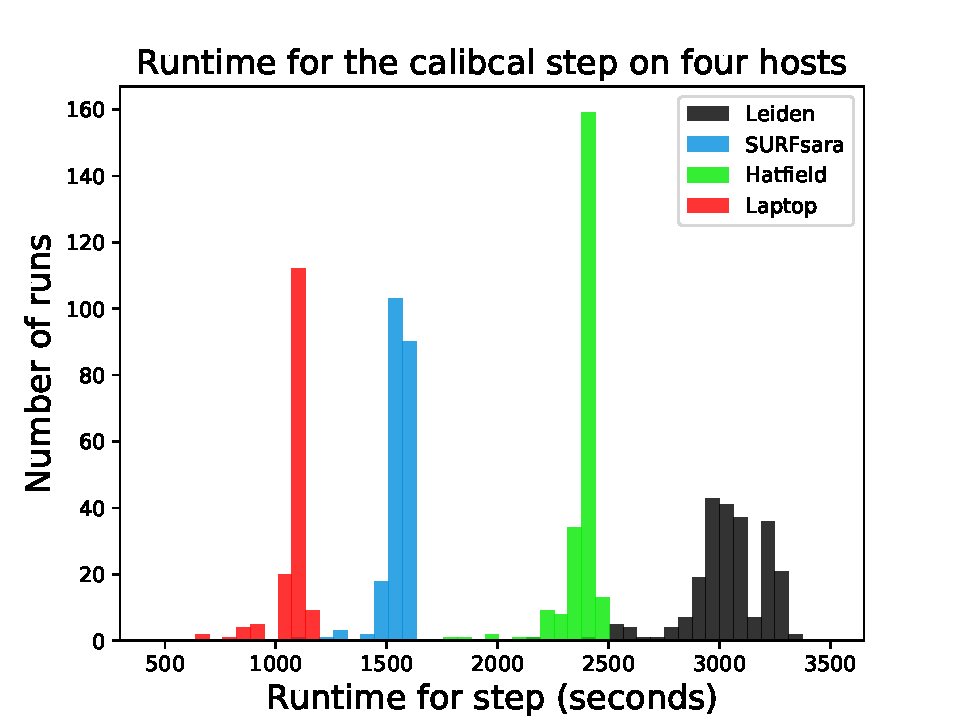
\includegraphics[width=\textwidth]{ch4/figures/fig3/figure3_calibcal.pdf}
    \caption{calib\_cal}
	\label{fig:ch4_calib_cal_bar}
 \end{subfigure}%
 \begin{subfigure}{.45\linewidth}
  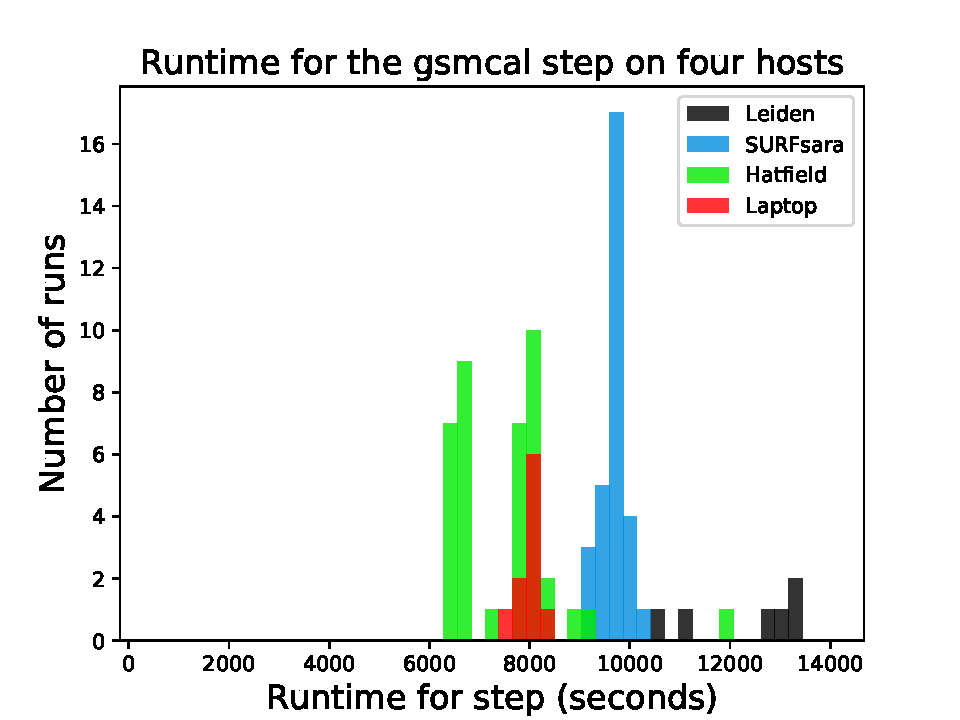
\includegraphics[width=\textwidth]{ch4/figures/fig3/fixed-figure3_gsmcal.pdf}
  \caption{\textit{gsmcal\_solve} }
  \label{fig:ch4_gsmcal_bar}
 \end{subfigure}
    \caption[Job completion times for two processing steps tested on four hardware setups]{Job completion times for \textit{calib\_cal} and \textit{gsmcal\_solve} steps tested on four hardware setups. The \textit{calib\_cal} step ran 244 times. The \textit{gsmcal\_solve} ran 24 times as the data is concatenated from 244x1 to 24x10 sets.  The step with the longest latency is \textit{gsmcal\_solve} while \textit{calib\_cal} consumes a comparable number of core-hours over 244 jobs. } 
  \label{fig:ch4_calibcal_fitclock_bars}
\end{figure*}

\begin{figure*}
  \centering
     \begin{subfigure}{.45\linewidth}
    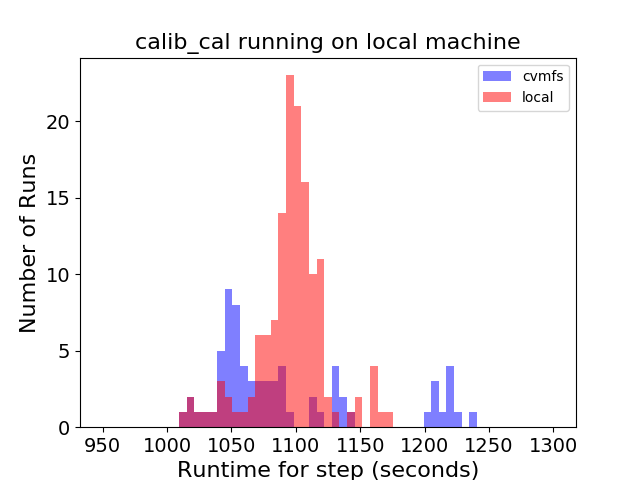
\includegraphics[width=\linewidth]{ch4/figures/ppr2_calib_local.png}
    \caption{Two compilation options on a Laptop}
	\label{fig:ch4_cmvfs1_calib}
    \end{subfigure}%
    \begin{subfigure}{.45\linewidth}
     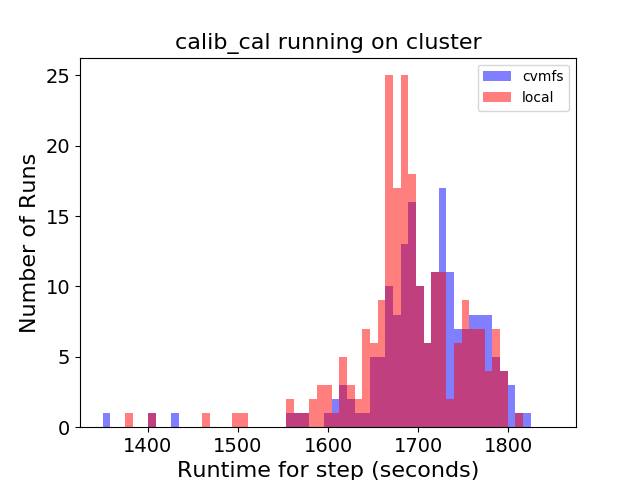
\includegraphics[width=\linewidth]{ch4/figures/ppr2_calib_cluster.png}
    \caption{Two compilation options on cluster node}
	\label{fig:ch4_cmvfs2_calib}
    \end{subfigure}%
      \caption[Speed comparison between natively and remotely compiled software for the 'calib\_cal' step.]{Difference in processing time for \textit{calib\_cal} when compiled remotely and natively. \textit{calib\_cal} was run 244 times with the native software and 40 times with the CVMFS compilation. Two tests were done, one on the personal laptop (\ref{fig:ch4_cmvfs1_calib}) and one on a cluster node at the LIACS Data Science Lab (\ref{fig:ch4_cmvfs2_calib}). The test on a cluster node shows no significant difference in run time between compilation options. The laptop test suggests that the remotely compiled software may run 5\% faster than the local compilation. } 
	\label{fig:ch4_cvmfs_native}
\end{figure*}


\begin{figure*}
  \centering
     \begin{subfigure}{.45\linewidth}
    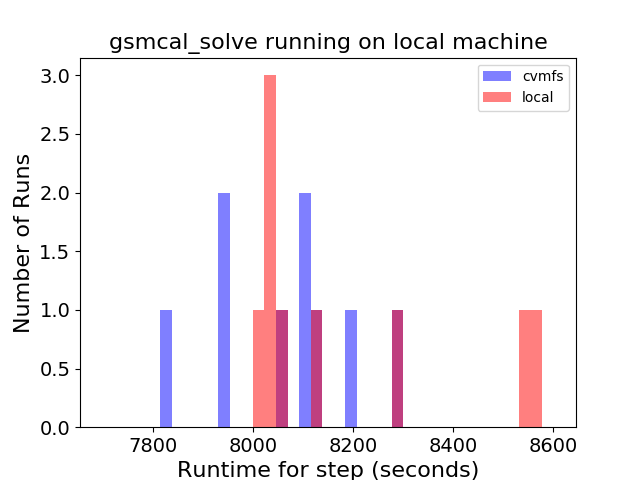
\includegraphics[width=\linewidth]{ch4/figures/ppr2_gsm_local.png}
    \caption{Two compilation options on a Laptop}
	\label{fig:ch4_cmvfs1_gsmcal}
    \end{subfigure}%
    \begin{subfigure}{.45\linewidth}
     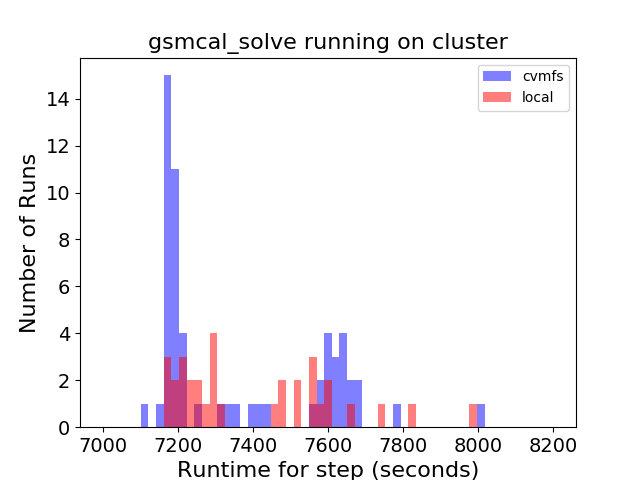
\includegraphics[width=\linewidth]{ch4/figures/ppr2_gsm_cluster.png}
    \caption{Two compilation options on cluster node}
	\label{fig:ch4_cmvfs2_gsmcal}
    \end{subfigure}%
      \caption[Speed comparison between natively and remotely compiled software for the 'gsmcal\_solve' step.]{Difference in processing time for \textit{gsmcal\_solve} when compiled remotely and natively. \textit{gsmcal\_solve} was run 50 times with the native software and 120 times with the CVMFS compilation. Two tests were done, one on the personal laptop (\ref{fig:ch4_cmvfs1_gsmcal}) and one on a cluster node at the LIACS Data Science Lab (\ref{fig:ch4_cmvfs2_gsmcal}). Just like with the \textit{calib\_cal} step, the \textit{gsmcal\_solve} step also doesn't accelerate significantly when natively compiled.} 
	\label{fig:ch4_cvmfs_native_gsm}
\end{figure*}

\subsection{Prefactor Run time and Hardware Parameters}\label{sec:ch4_res_tcoll}

Next, we studied the dependence of run time on different hardware parameters. With software that collects per-step performance statistics for the LOFAR pipeline, the dependence of the pipeline processing on hardware performance can be easily profiled and studied. Using \textit{pipeline\_collector} we determined the pipeline's slowest steps with respect to different hardware parameters. 

The system parameters studied here are the CPU speed, memory throughput, cache size and disk speed. Modern computers can have a complex memory hierarchy as demonstrated in Figure \ref{fig:ch4_mem_hiearch} \citep{mem_hiearch}. This is due to the cost trade-off between memory size and memory speed. Because of this trade-off, the full data set is stored on disk, while the working set is placed in RAM. This is the data that the processor needs to access at the current time \citep{workingset}. The most frequently accessed parts of the data are stored in the CPU cache, which evicts the oldest data when full \citep{cache_eviction}. 

The CPU processing speed is faster than the RAM latency, so a hierarchy of caches exist. Caches store small subsets of the working set and have a fast connection to the processor. The fastest data link is between the CPU and the L1 Cache, with the link to RAM being slower and the disk read speed slower still. The limited memory capacity of the different levels of the memory hierarchy  as well as the throughput between them will lead to performance bottlenecks. These bottlenecks will lead to the processor waiting on memory. Such stalls lead to longer processing times.

\begin{figure}[ht!]
  \centering
    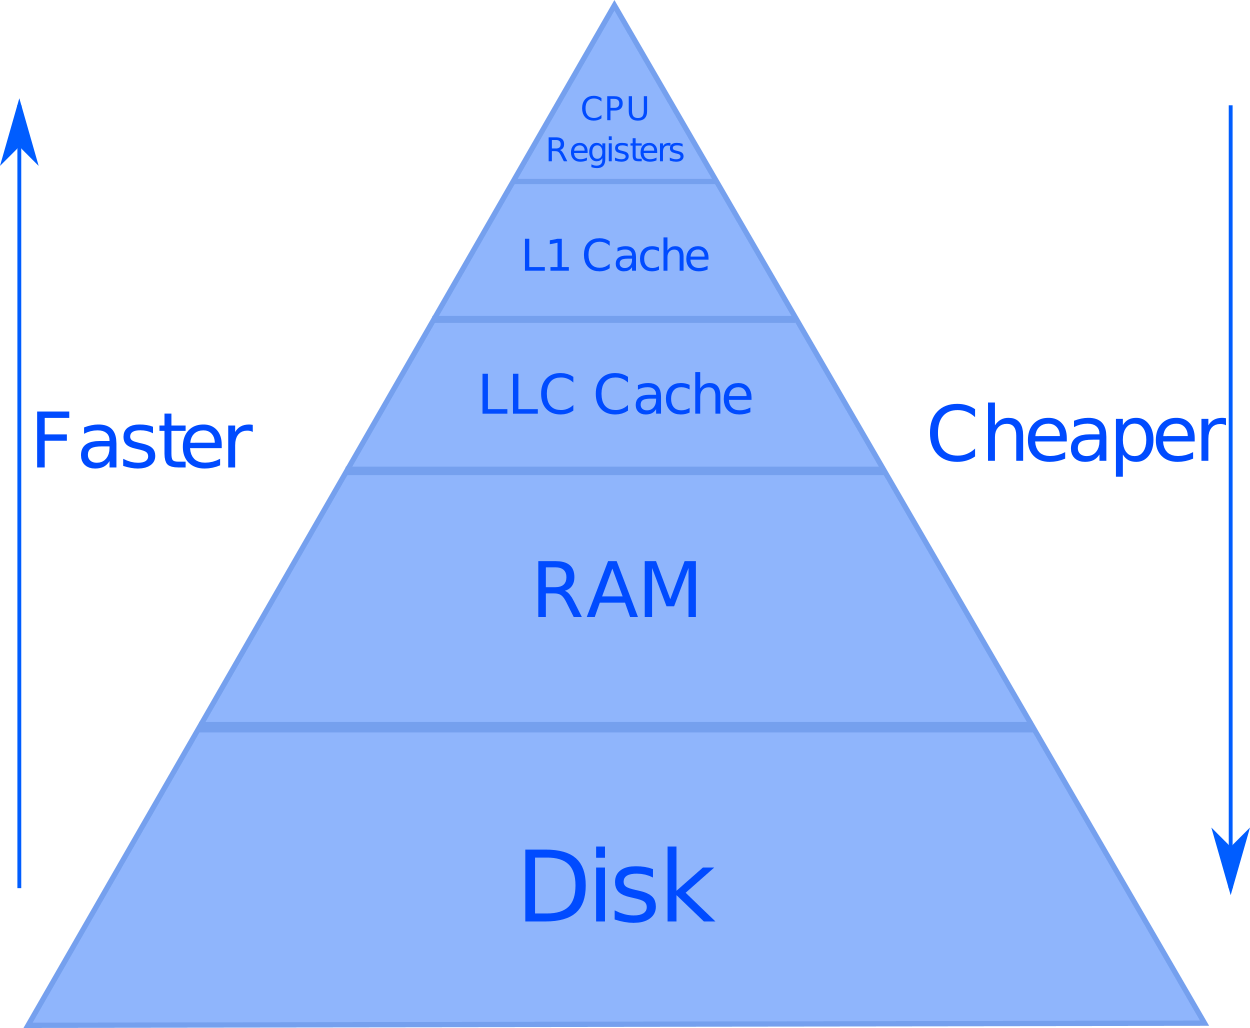
\includegraphics[width=0.5\linewidth]{ch4/figures/fig6/pyramid.png}
      \caption{A model of the memory hierarchy, as described in \citep{goto2008anatomy}. }
	\label{fig:ch4_mem_hiearch}
\end{figure}


\subsubsection{CPU}
The CPU speed is usually the primary factor determining how fast computations can be made. In general, a faster CPU will result in faster data processing. 

However, Fig. \ref{fig:ch4_calib_cal_CPU} shows that the run time of the calibration of the calibrator does not strongly depend on the CPU frequency. While the test nodes at SURFsara and Leiden run at the same CPU frequency, running on a cluster node at SURFsara takes half the time as on a node at Leiden. Even more surprisingly, the \textit{gsmcal\_solve} step does not benefit significantly from a faster CPU, despite being the most computationally heavy \textit{prefactor} step (\textbf{R2}). This step does the gain calibration on the target field using the StEFCal algorithm \citep{stefcal}. Figure \ref{fig:ch4_gsmcal_CPU} shows only a slight improvement over faster CPU clock speeds for both steps. The correlation between completion time and CPU speed is similar for both steps.

\begin{figure*}
    \centering
\begin{subfigure}[b]{0.45\linewidth}
%\begin{subfigure}{.5\textwidth}
    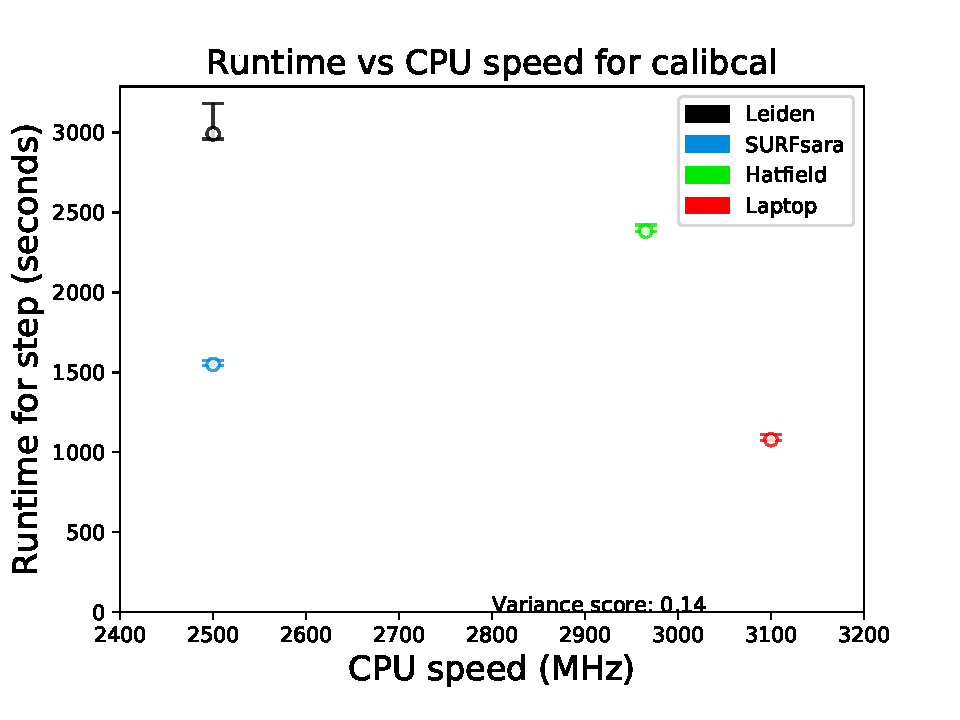
\includegraphics[width=\linewidth]{ch4/figures/fig7/calibcalCPU.pdf}
      \caption{calib\_cal }
	\label{fig:ch4_calib_cal_CPU}
 \end{subfigure}%
 \begin{subfigure}[b]{0.45\linewidth}
    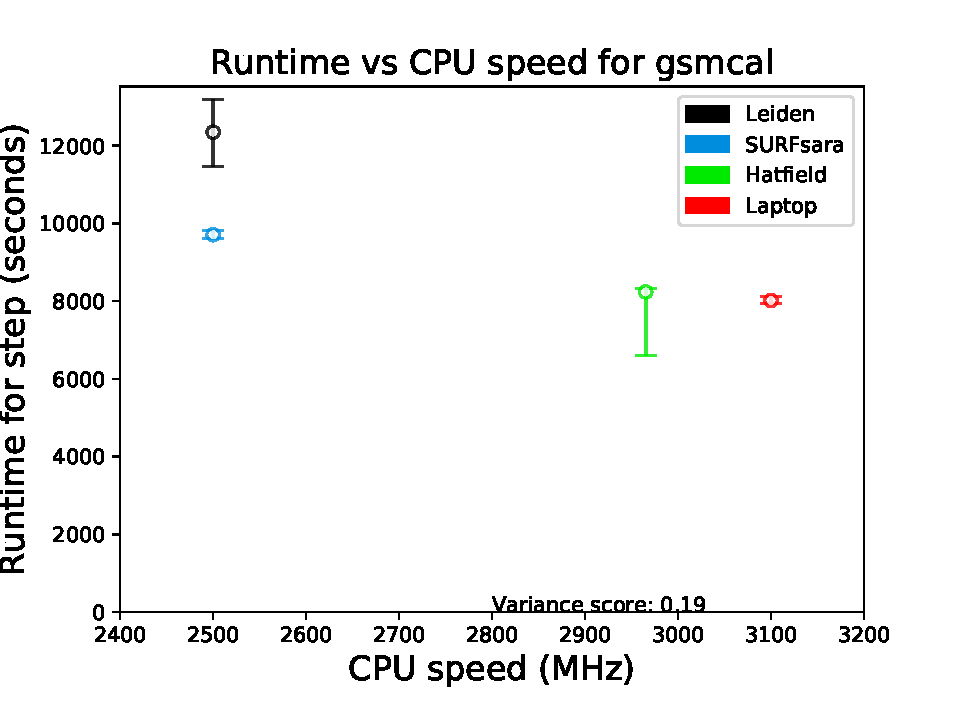
\includegraphics[width=\linewidth]{ch4/figures/fig7/gsmcalCPU.pdf}
      \caption{\textit{gsmcal\_solve}}
	\label{fig:ch4_gsmcal_CPU}
 \end{subfigure}
 \label{fig:ch4_CPU_3_steps}
    \caption[Effect of CPU speeds on the bottle neck steps for the four test machines.]{Performance of the bottleneck steps compared with the CPU speeds of the four test machines. The values are the mean of 244 runs (Standard prefactor run) and the error bars show the 1-sigma of the distribution of the run time. } 

\hfill        %
\end{figure*}

\subsubsection{Cache}
The CPU has a hierarchy of caches consisting of Level 1, Level 2 Cache and LLC Cache. For the four processors tested, the Level 1 and 2 caches were all the same size, thus the only difference is the Last Level Cache (LLC or just Cache in Figure \ref{fig:ch4_mem_hiearch}). This cache stores data needed by the CPU, so the larger it is, the less the processor needs to wait for RAM to return data. 

In general, numerical codes benefit from larger cache sizes \citep{skadron1999branch,goto2008anatomy}. Interestingly,  figure \ref{fig:ch4_gsmcal_cache} suggests that the \textit{gsmcal\_solve} step does not exclusively depend on larger cache \textbf{R3} (Table \ref{table:ch4_results}). On the machines with a larger cache, the \textit{gsmcal\_solve} step completed processing as quickly as on the machines with smaller cache, even down to 8MB.  

\begin{figure*}
    \centering
    \begin{subfigure}[b]{0.45\linewidth}
    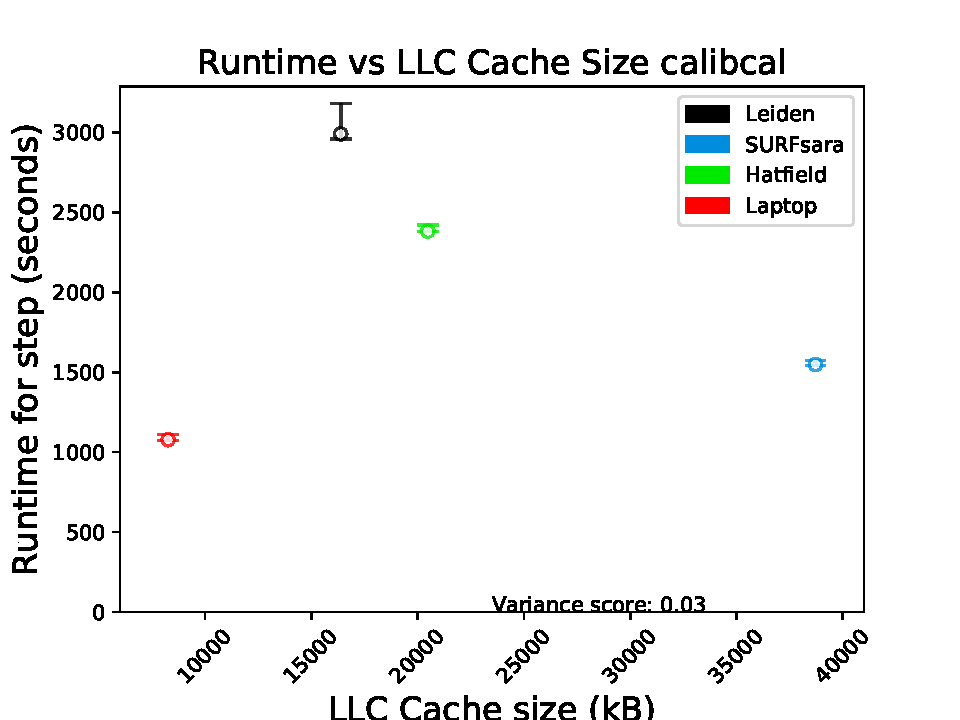
\includegraphics[width=\linewidth]{ch4/figures/fig8/calibcal_LLC.pdf}
      \caption{calib\_cal }
	\label{fig:ch4_calib_cal_cache}
 \end{subfigure}%
 \begin{subfigure}[b]{0.45\linewidth}
    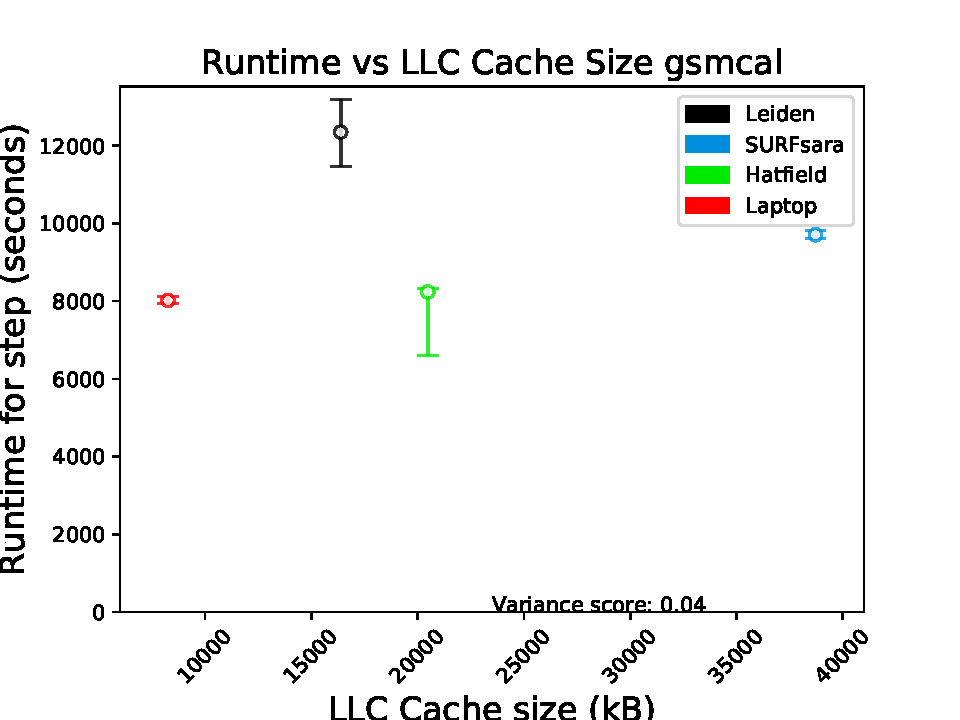
\includegraphics[width=\linewidth]{ch4/figures/fig8/gsmcal_LLC.pdf}
      \caption{\textit{gsmcal\_solve}}
	\label{fig:ch4_gsmcal_cache}
 \end{subfigure}
 \label{fig:ch4_cache_3_steps}
    \caption[Effect of cache size on the bottle neck steps for the four test machines.]{Performance of the two bottleneck steps with respect to Last Level Cache size. The \textit{gsmcal\_solve} step shows no trend between cache size and completion time. The \textit{calib\_cal} step runs the fastest on the machine with the smallest cache.  } 

\end{figure*}

\subsubsection{RAM Bandwidth}

If the entire data set does not fit into cache, the software needs to transfer data from RAM to the CPU. In these cases,  \textit{prefactor} benefits from a fast bandwidth between the cache and RAM. For this study, the RAM throughput was benchmarked\footnote{Using the command \texttt{\$> dd if=/dev/zero of=/dev/shm/test  bs=1M count=2048}}. This command copies dummy data into system memory. As this utility exists on all Unix systems, this is a standardized benchmark of the RAM performance. 

\begin{figure*}
\centering
    \begin{subfigure}[b]{0.45\linewidth}
    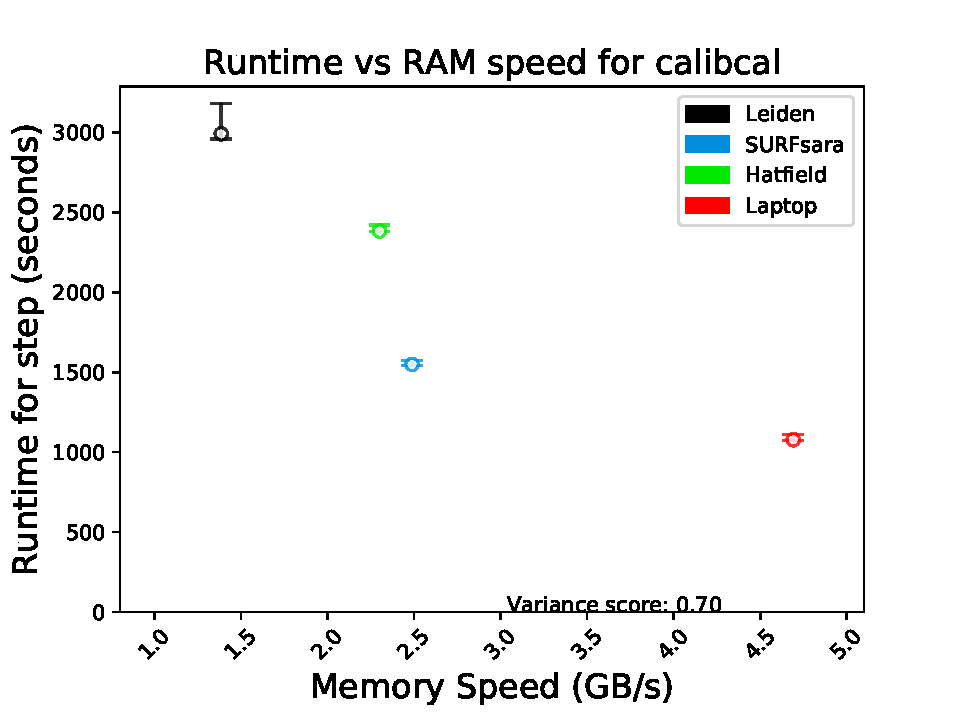
\includegraphics[width=\linewidth]{ch4/figures/fig9/calibcal_MEM.pdf}
      \caption{\textit{calib\_cal}}
	\label{fig:ch4_calib_cal_RAM}
 \end{subfigure}%
    \begin{subfigure}[b]{0.45\linewidth}
    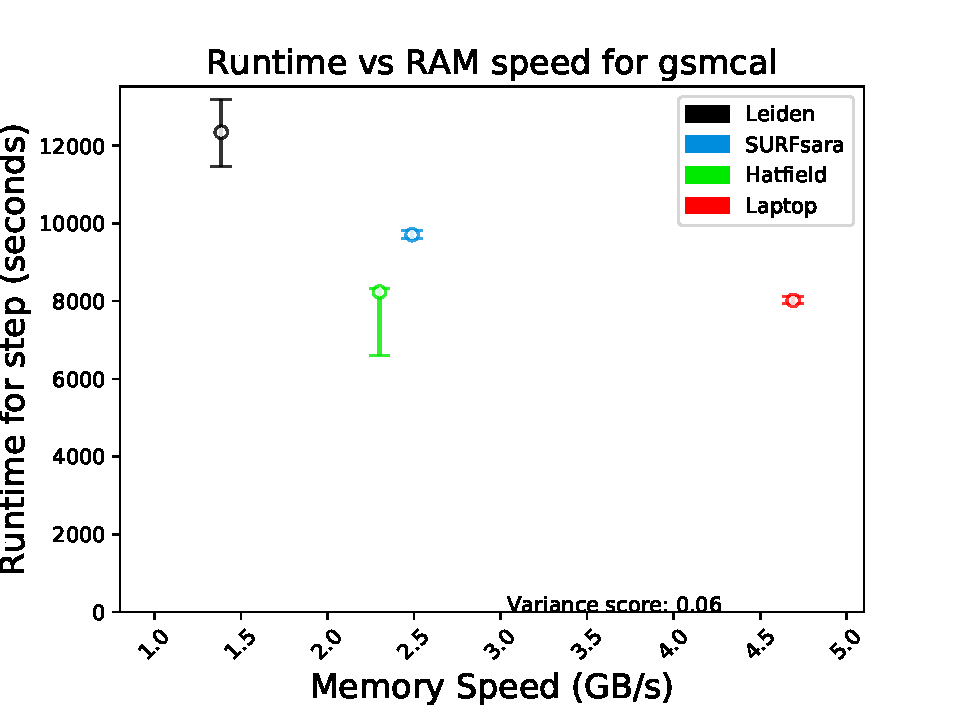
\includegraphics[width=\linewidth]{ch4/figures/fig9/gsmcal_MEM.pdf}
      \caption{\textit{gsmcal\_solve}}
	\label{fig:ch4_gamcal_RAM}
 \end{subfigure}
 \label{fig:ch4_ram_bandw}
    \caption[Effect of RAM throughput on the bottle neck steps for the four test machines.]{Performance of the two bottleneck steps and RAM bandwidth in GB/s. Both the \textit{calib\_cal} and \textit{gsmcal\_solve} steps show a trend of faster processing times on machines with higher RAM bandwidth. Both steps show a trend of decreasing processing time with increasing RAM throughput.} 
\end{figure*}

Figure \ref{fig:ch4_calib_cal_RAM} showed that higher bandwidth is correlated with a faster completion time for the \textit{calib\_cal} and \textit{gsmcal\_solve} steps (\textbf{R4}). The result is to be expected as the working set of these steps is 200MB and 1.0GB respectively, and cannot fit into cache readily, however it is loaded into RAM within the first 5 seconds of the run (Figure \ref{fig:ch4_VMRSS}), and is streamed from memory throughout the run. 

\subsubsection{Disk Read speeds}

The slowest link in the memory hierarchy is the disk read speed. For the \textit{calib\_cal} step, the entire data is loaded into memory during the first few seconds of the run, after which the disk only becomes important when the results need to be written out. The \textit{gsmcal\_solve} step streams data from the disk to memory throughout the entire run.  The plot of disk read speeds (Fig. \ref{fig:ch4_gsmcal_HDD}) also shows that a faster disk does not speed up the slowest step \textbf{R5}. To verify that disk throughput was not the limiting factor, the entire data set (25 GB) was moved to main memory (using /dev/shm).  The resulting run time for both bottleneck steps did not change.  

The calibration steps both stored less than 200MB of data in memory throughout their run. Figure \ref{fig:ch4_VMRSS} shows the time-series of the total memory used by these steps. The \textit{calib\_cal} step uses only 200MB of memory and \textit{gsmcal\_solve} only 35MB. While the \textit{gsmcal\_solve} step works on a 1GB data set, it streams the data in memory and thus does not require 1GB of RAM. Alternatively, the \textit{calib\_cal} step loads the entire (200MB) data set into memory for the entire duration of the run. The RAM usage time-series in Figure \ref{fig:ch4_VMRSS} show that the RAM is filled for the first 5 seconds of the run, further confirming that the processing is effectively independent from disk speed. 


\begin{figure*}
  \centering
   \begin{subfigure}{.45\textwidth}
    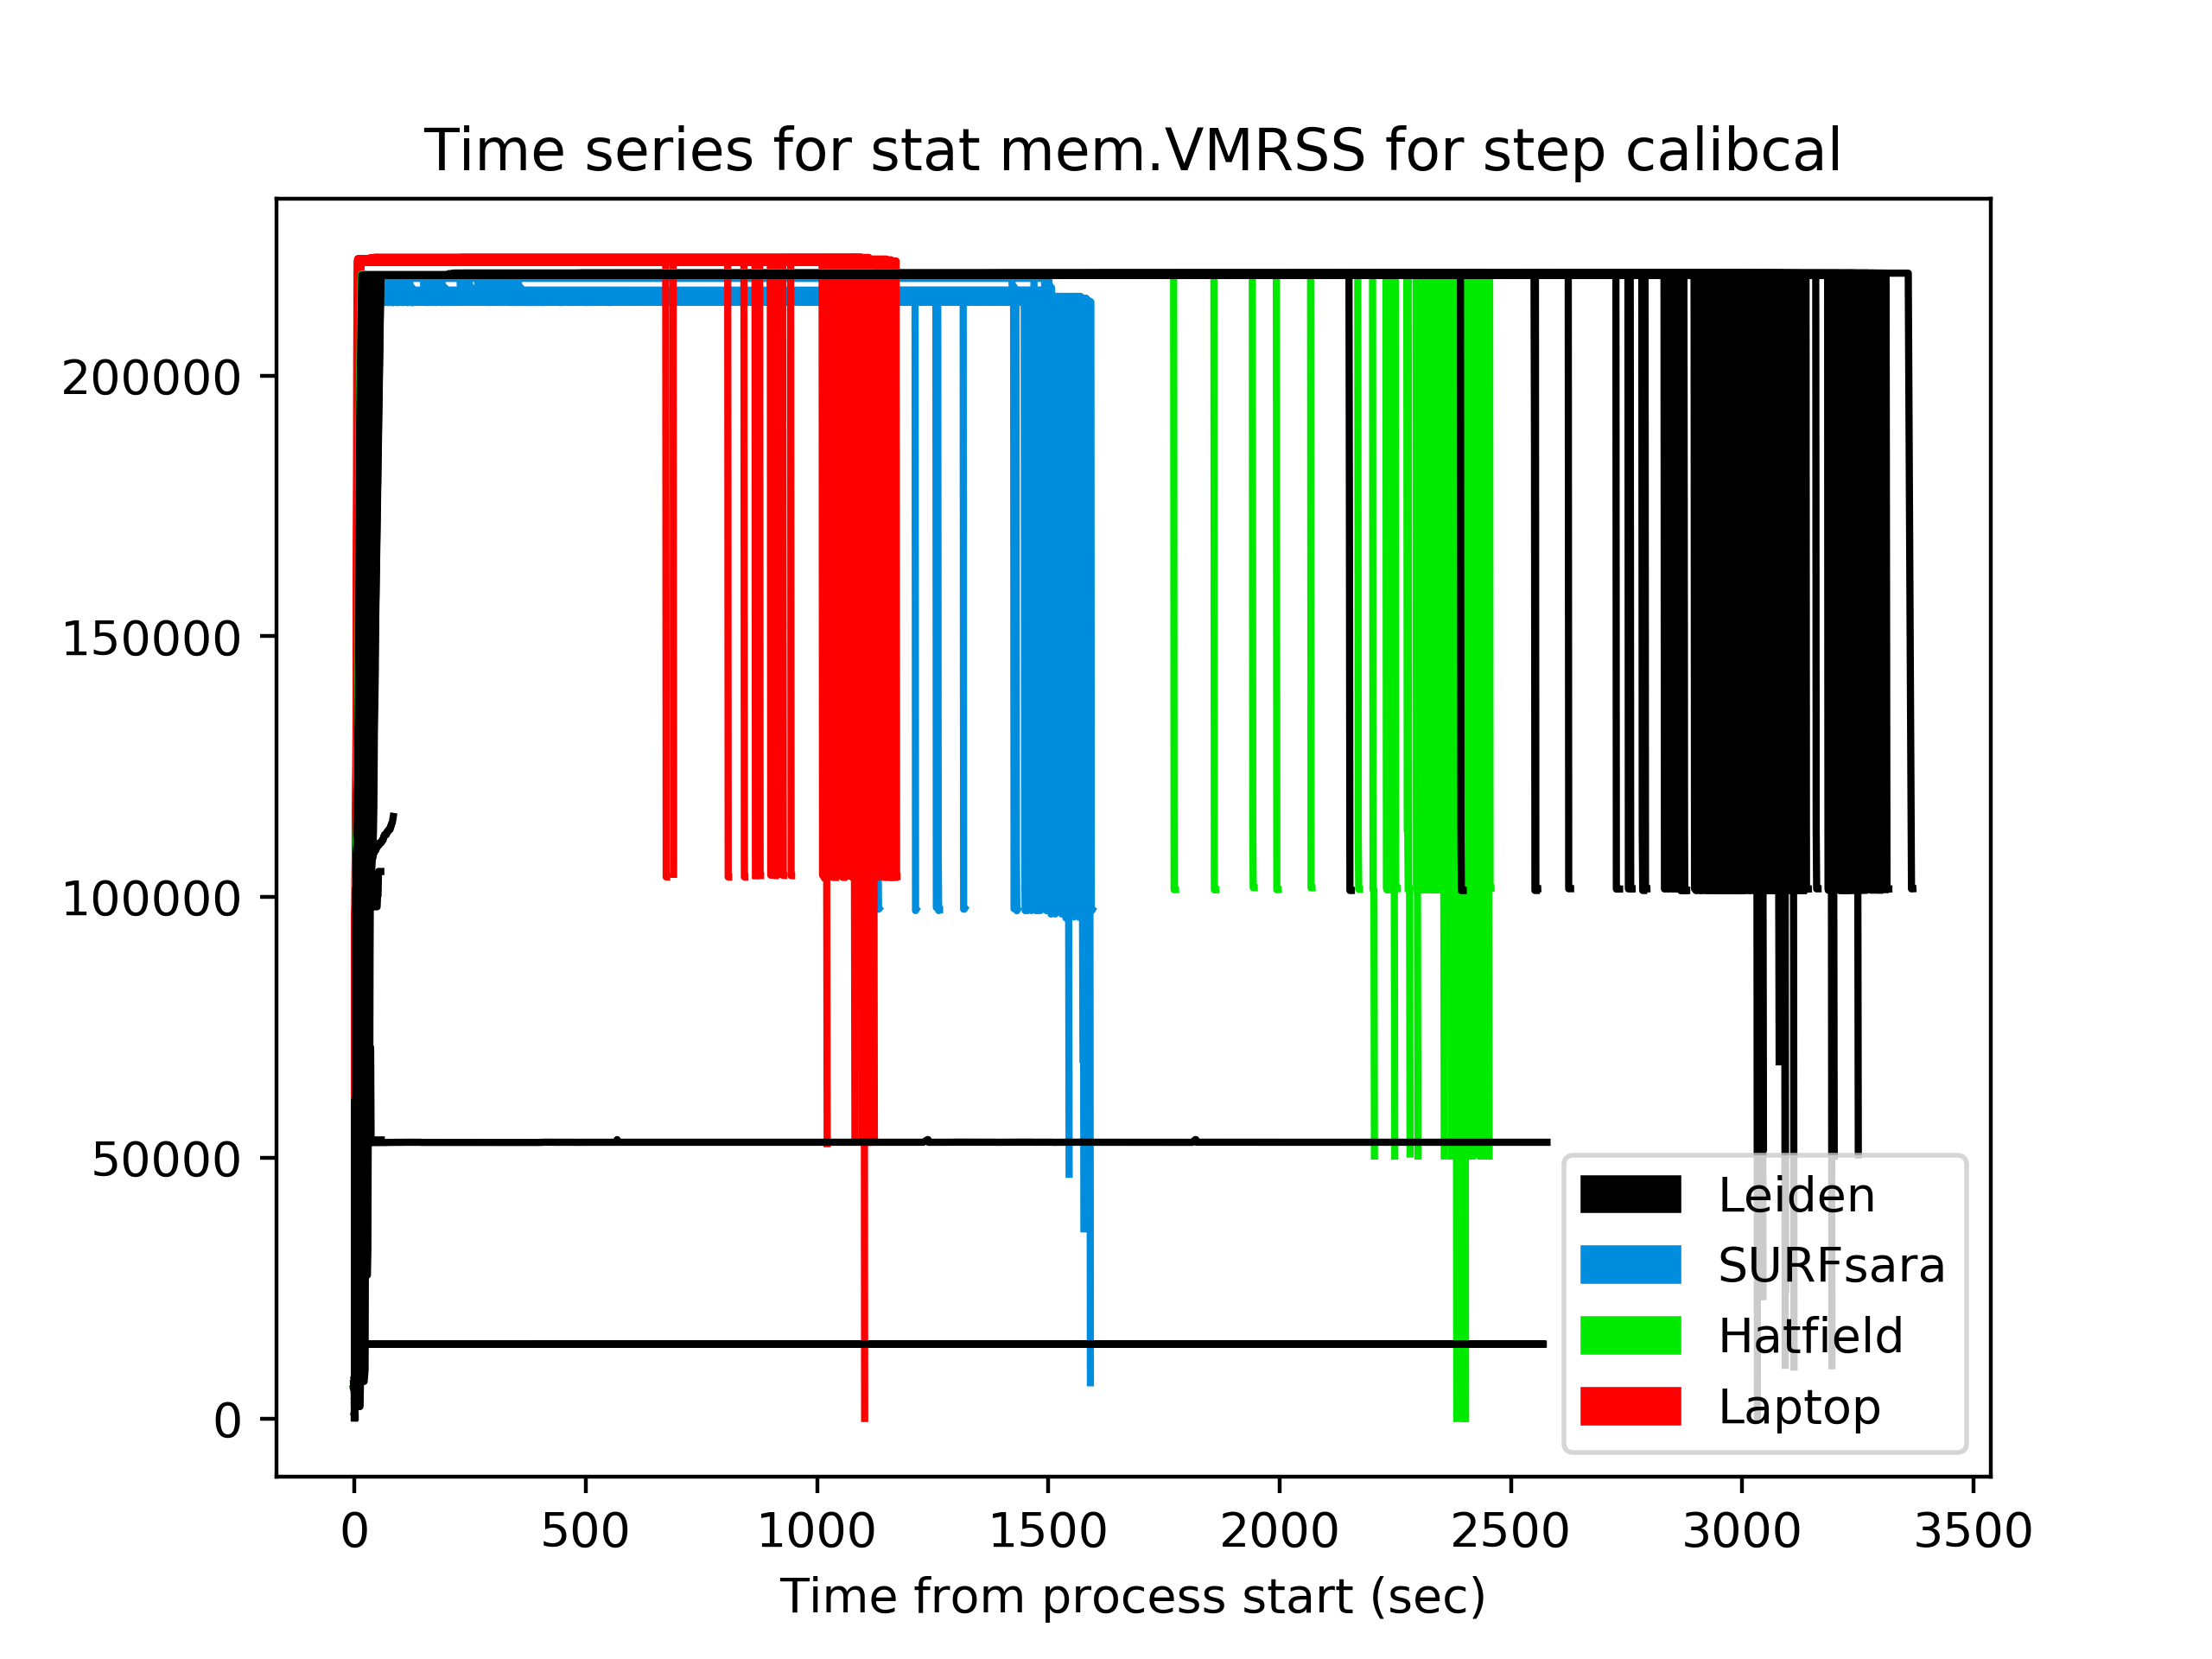
\includegraphics[width=\textwidth]{ch4/figures/fig10/calibcal_vmrss.png}
      \caption{\textit{calib\_cal} }
	\label{fig:ch4_calib_cal_VMRSS}
 \end{subfigure}%
 \begin{subfigure}{.45\textwidth}
    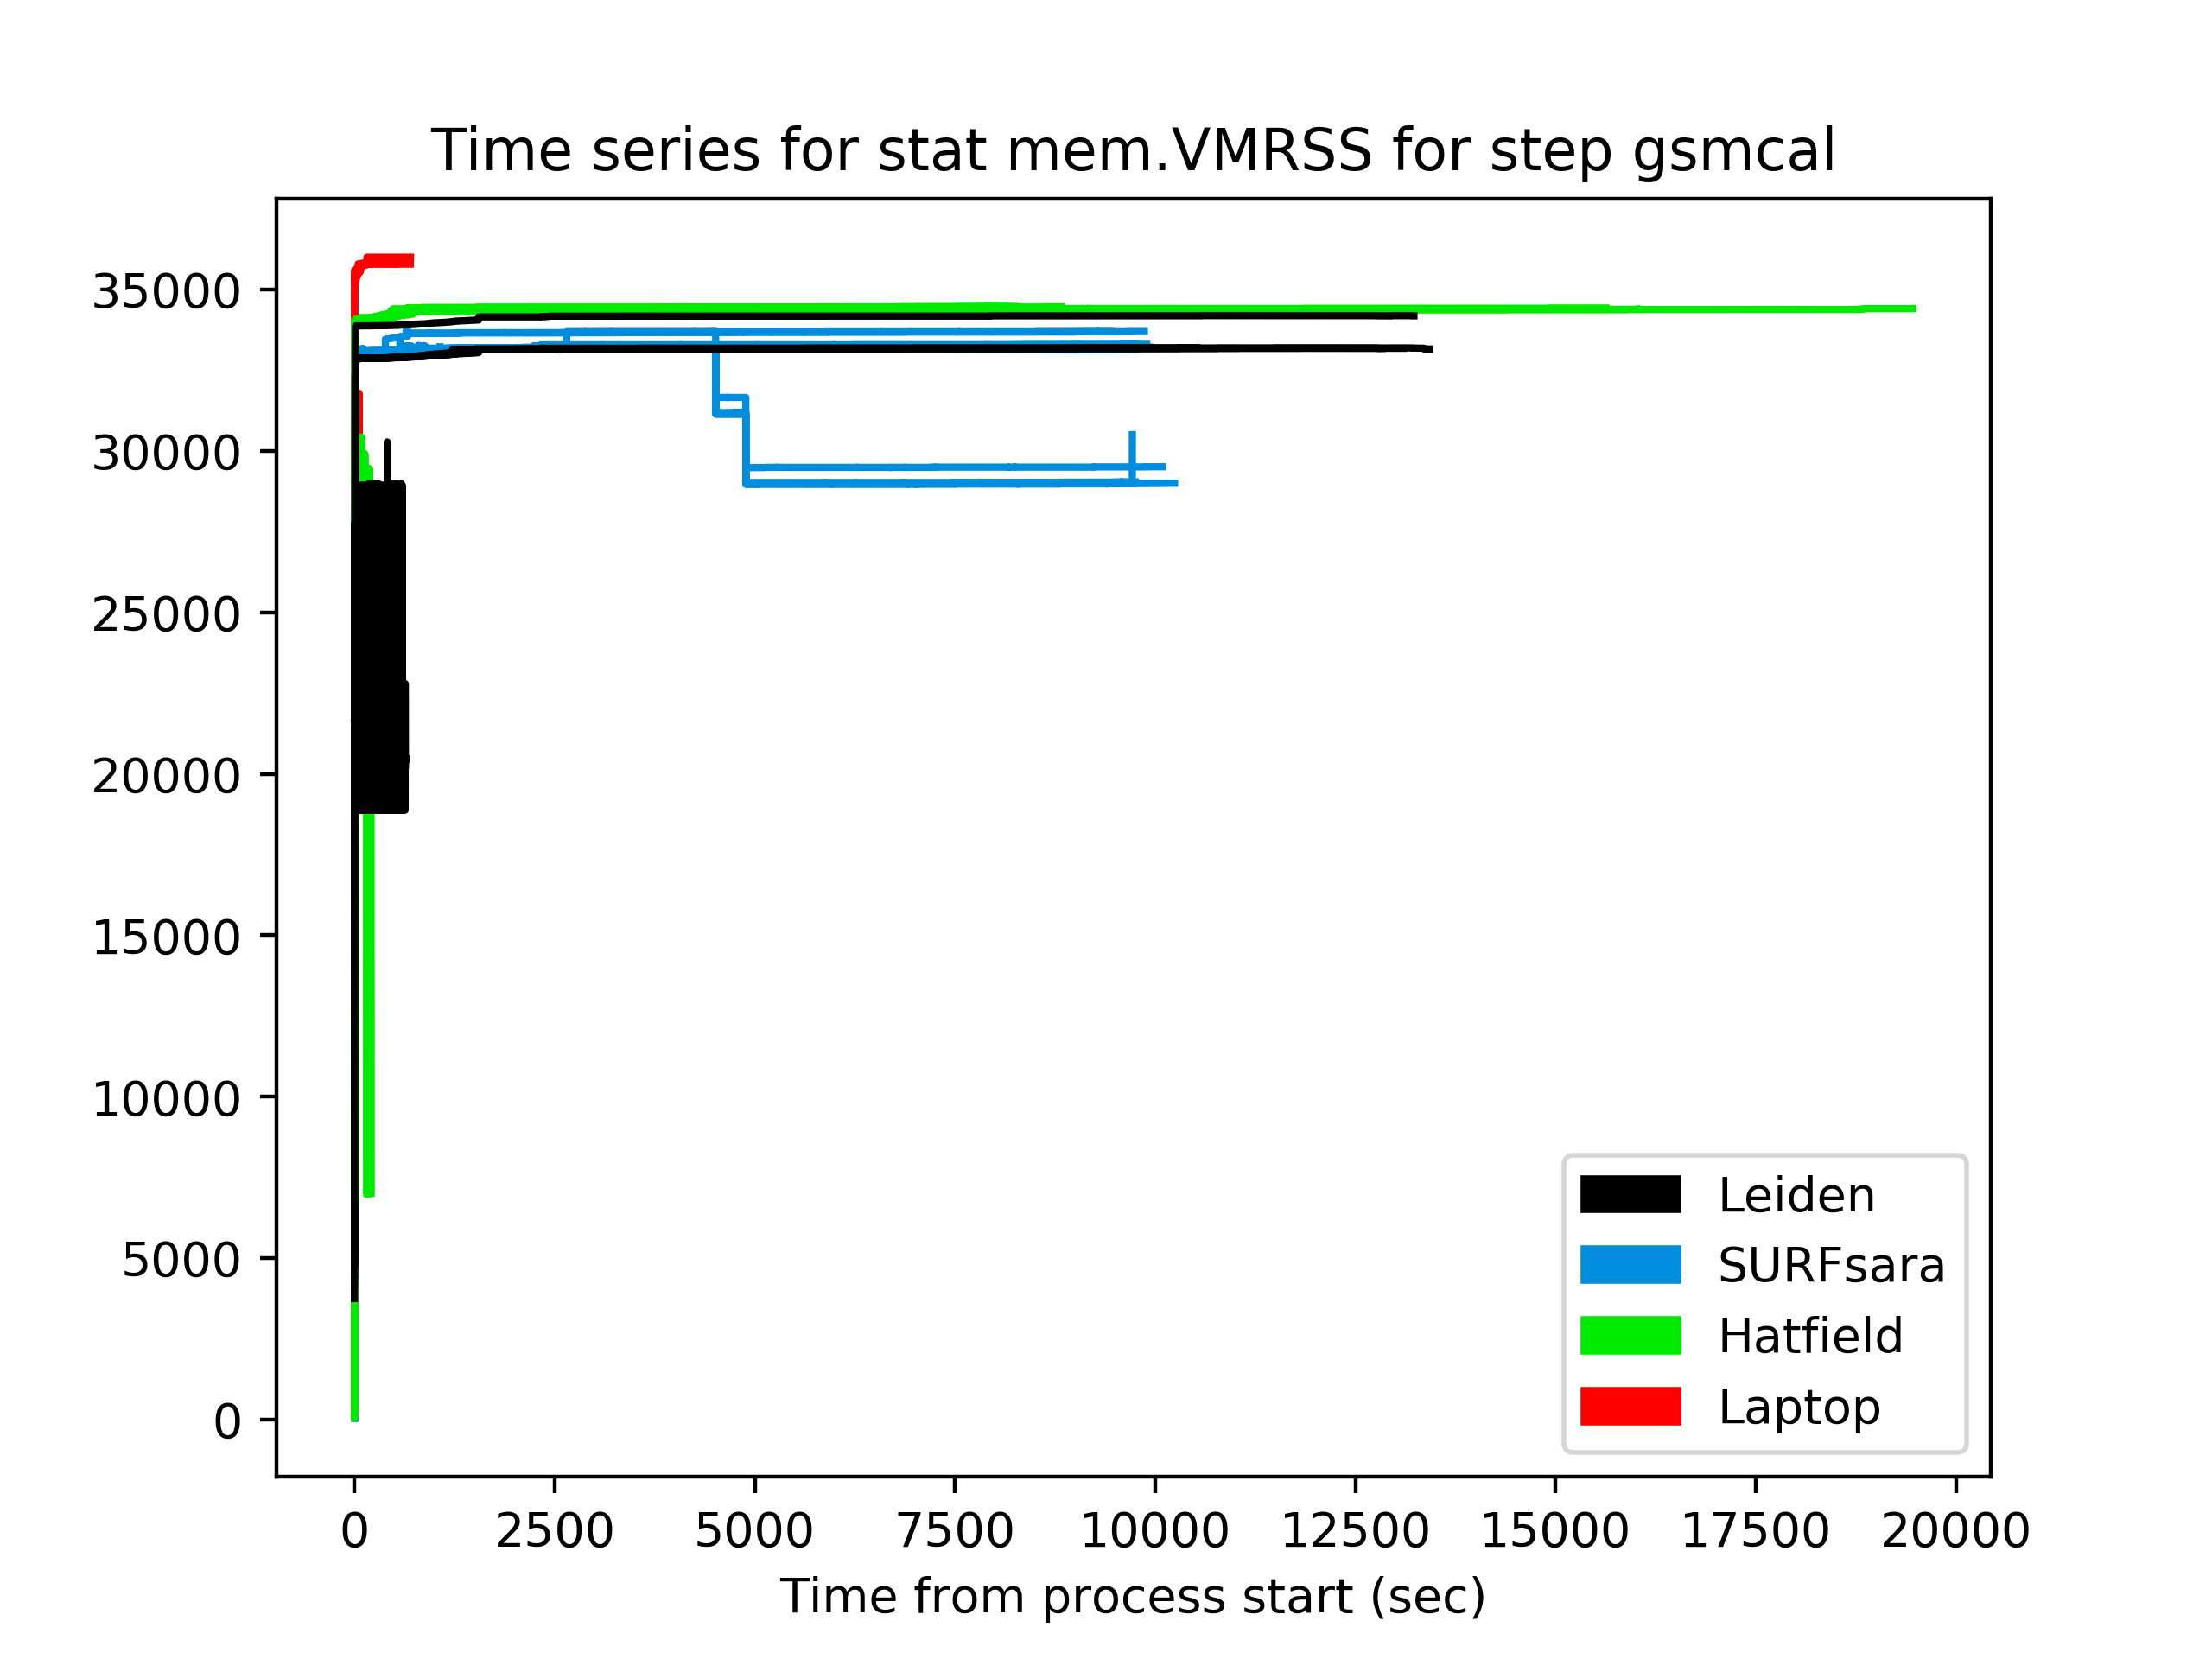
\includegraphics[width=\textwidth]{ch4/figures/fig10/gsmcal_vmrss.png}
      \caption{\textit{gsmcal\_solve}}
	\label{fig:ch4_fitclock_VMRSS}
 \end{subfigure}
    \caption[Time series of the Virtual Memory Resident Set Size]{Time series of the Virtual Memory Resident Set Size. This is the amount of data stored in RAM (in Kb) during the \textit{calib\_cal} and \textit{gsmcal\_solve} steps. Both steps show the same amount of memory use on all test machines. Additionally, after a brief loading of data, the memory usage remains constant until processing is finished. }
 \label{fig:ch4_VMRSS}
\end{figure*}

\begin{figure}
  \centering
   \begin{subfigure}{.45\textwidth}
    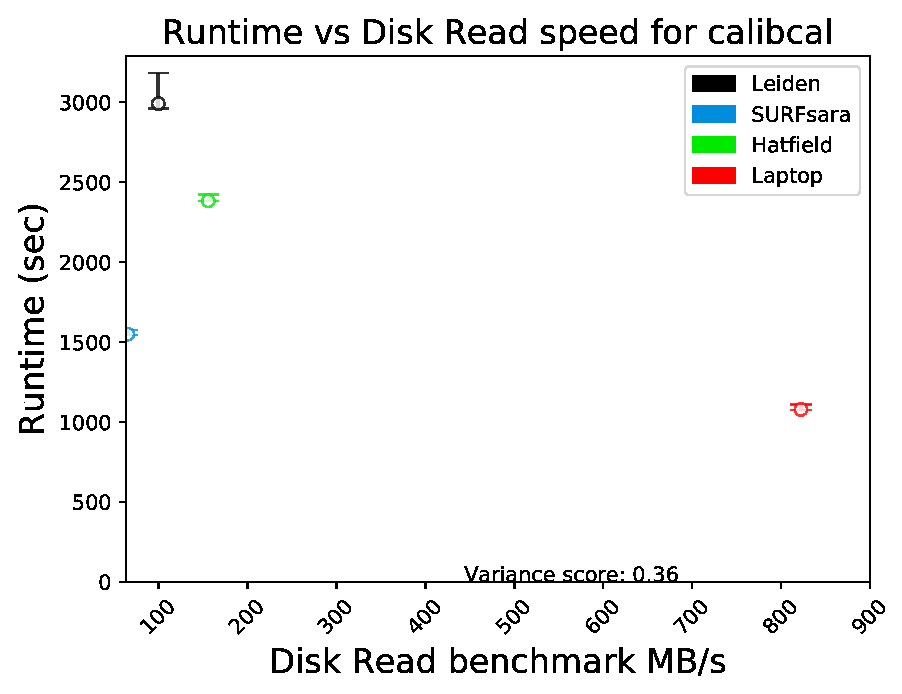
\includegraphics[width=\textwidth]{ch4/figures/fig11/calibcal_HDD.eps}
      \caption{calib\_cal }
	\label{fig:ch4_calib_cal_HDD}
 \end{subfigure}
  \begin{subfigure}{.45\textwidth}
    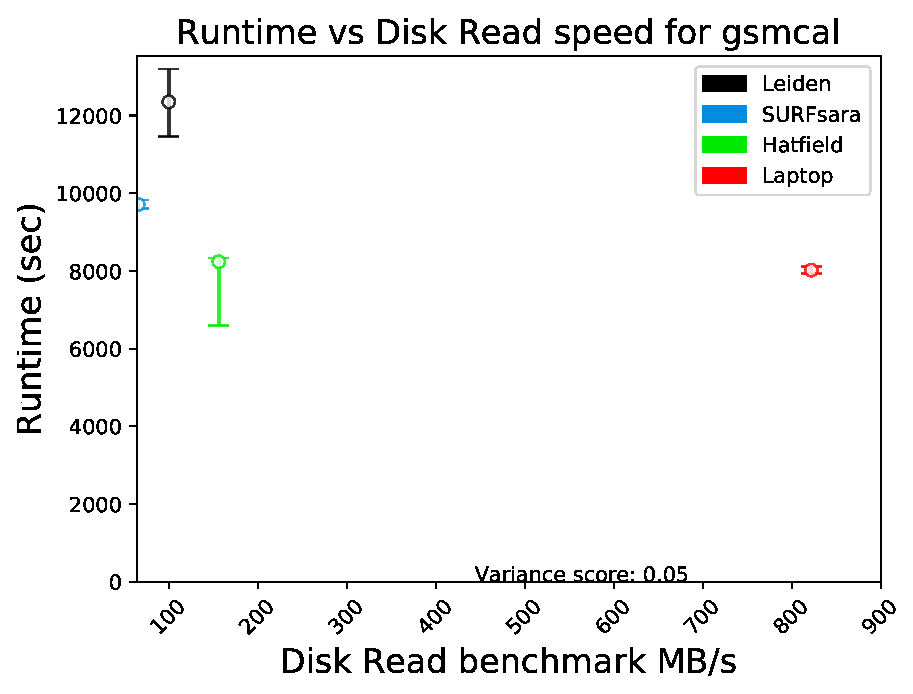
\includegraphics[width=\textwidth]{ch4/figures/fig11/GSMcal_HDD.eps}
      \caption{\textit{gsmcal\_solve}}
	\label{fig:ch4_gsmcal_HDD}
 \end{subfigure}
 \label{fig:ch4_HDD_2_steps}
    \caption[Performance of the two bottleneck steps and Disk bandwidth in MB/s.]{Performance of the two bottleneck steps and Disk bandwidth in MB/s. There is no correlation between the Disk read speed and the Run time of the steps.} 
\end{figure}


\section{CPU Utilization Tests with PAPI}\label{sec:ch4_PAPI}

To gain more fine grained data on the CPU utilization, the \textit{calib\_cal} and \textit{gsmcal\_solve} steps were tested with the PAPI package.  We ran this package as a test, to determine whether collecting PAPI data is helpful in understanding pipeline performance.  PAPI can record data such as cache performance, branch prediction rate, fraction of memory/branch instructions and others. This data is complementary to the procfs information, which is collected by the Linux kernel. As the collected data was useful in understanding the \textit{prefactor} pipeline, we will include PAPI in the \textit{pipeline\_collector} suite in the future. In the following sections we will discuss the results obtained for the \textit{calib\_cal} and \textit{gsmcal\_solve} steps.

\subsection{Level 1 Data Misses}

The Level 1 Cache is split into cache for instructions and data. For all our test hardware the L1 Data cache is 32 Kb, and has a direct link to the processor's computational units \citep{haswell}. The processor collects information logging how many times data requested by the CPU is not located into the L1 Data cache. This counter is called the Level 1 Data Cache Miss rate. To resolve this type of cache miss, the data needs to be fetched from L2 Cache. When this happens, the processor has to wait for the requested data. \textbf{R7}: The recorded L1 data misses in Figure \ref{fig:ch4_L1Dm}, show that the software performing the \textit{calib\_cal} step  misses 20\% of its L1 data cache requests, while the software implementing the \textit{gsmcal\_solve} step misses less than 5\% of L1 Cache requests. These cache misses often happens in multi-threaded applications where there are instructions shared by multiple threads on the same cache line \citep{cache_opt}. 

\begin{figure}
  \centering
      \begin{subfigure}{.45\textwidth}
      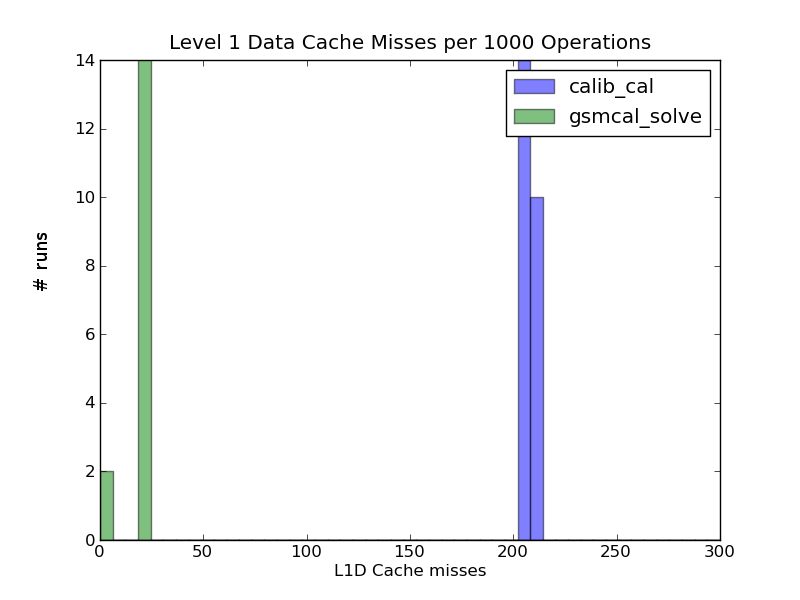
\includegraphics[width=\textwidth]{ch4/figures/L1D_miss.png}
      \caption{Level 1 Data cache misses }
	\label{fig:ch4_L1Dm}
    \end{subfigure}
    \begin{subfigure}{.45\textwidth}
    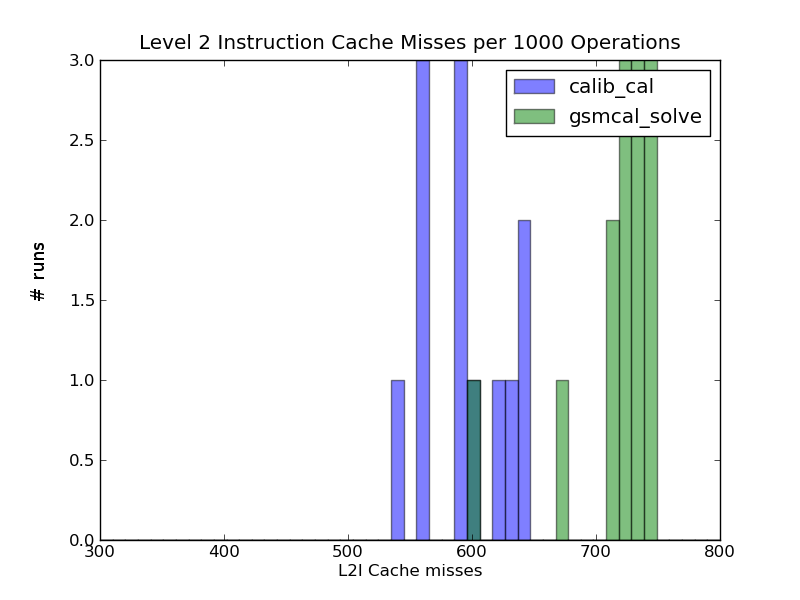
\includegraphics[width=\textwidth]{ch4/figures/L2I_miss.png}
      \caption{Level 2 Instruction cache misses }
	\label{fig:ch4_L2Im}
  \end{subfigure}
    \caption[Cache miss rates for the bottleneck steps, executed on the SURFsara gina cluster.]{Cache miss rates for \textit{calib\_cal} and \textit{gsmcal\_solve}, executed on the SURFsara gina cluster. The cache is split into instruction and data caches. The figures above show the difference in number of cache misses for both instruction cache and data cache for the slowest \textit{prefactor} steps. \textit{calib\_cal} suffers significantly more Data cache misses than \textit{gsmcal\_solve} while the two steps undergo similar instruction Cache misses.  }
\end{figure}


\subsection{Level 2 Instruction Misses}

Unlike the Level 1 cache, Level 2  cache stores data and instructions in the same location. When the cache is full, it evicts the last used element in order to make space for newly requested data. PAPI also counts these eviction events. 
Figure \ref{fig:ch4_L2Im} shows that for both steps, between 50 and 70\% of L2 requests for an instruction do not match the contents of L2 Cache. This is significantly more than the applications benchmarked in \citep[Table 2]{cache_misses}. Because both steps process data of considerable size, the large amount of data required can evict instructions from the L2 cache (insight number \textbf{R7} in table \ref{table:ch4_results}). 

\subsection{Resource Stalls}

Modern processors have multiple computational pipelines on chip, in order to process data in parallel \citep{pipeline_x86}. There are times when the processor's internal pipeline needs to wait for other instructions to finish. When this happens, it flags that it has 'stalled on a resource'. These resource stall cycles are also recorded by PAPI and represented as a percentage of total cycles. From figure \ref{fig:ch4_rstall}, it can be seen that \textit{calib\_cal} stalls on 70\% of the processor cycles, while  \textit{gsmcal\_solve} only on 33\% of cycles (\textbf{R8}). 

The Full Issue Cycles counter indicates the percentage of processor cycles, in which the theoretical maximum number of instructions are executed. During these cycles, the software uses the CPU optimally. The full issue cycles counter (Fig. \ref{fig:ch4_full_issue}) also shows the difference in efficiency between the \textit{calib\_cal} and \textit{gsmcal\_solve} step  (\textbf{R9}), with the former only working at peak efficiency for 10\% of the processor cycles.

\begin{figure}
  \centering
      \begin{subfigure}{.45\textwidth}
      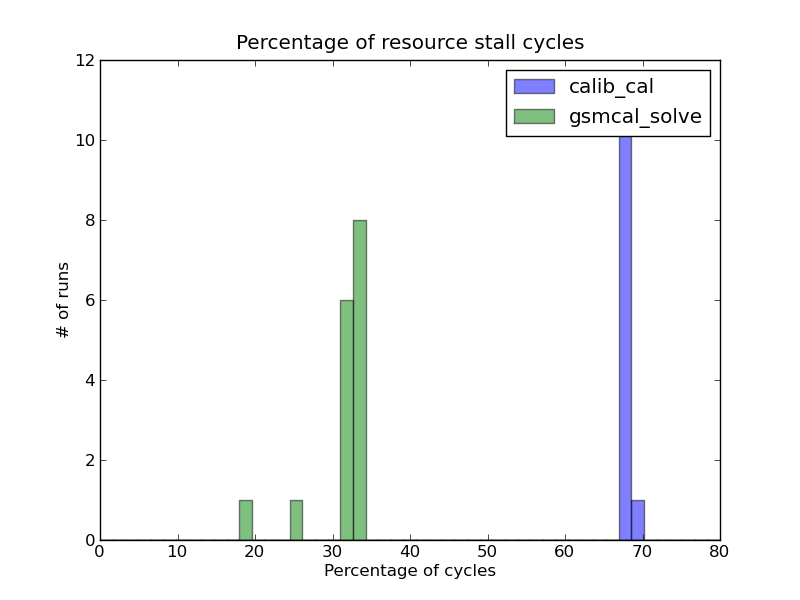
\includegraphics[width=\textwidth]{ch4/figures/rstall.png}
      \caption{Resource Stall Cycles}
	\label{fig:ch4_rstall}
    \end{subfigure}
    \begin{subfigure}{.45\textwidth}
    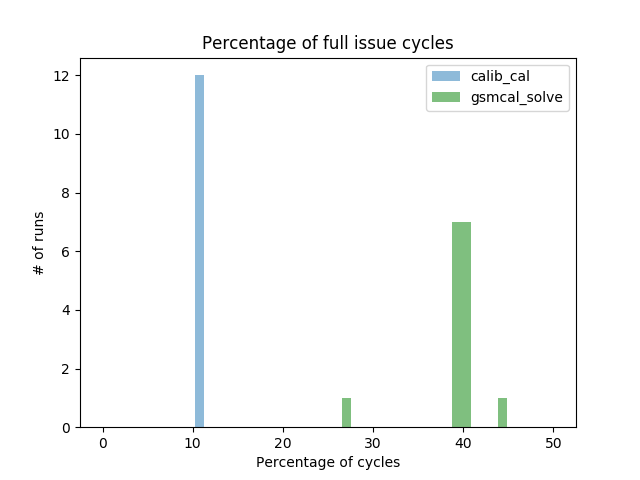
\includegraphics[width=\textwidth]{ch4/figures/full_issue.png}
      \caption{Full Issue cycles }
	\label{fig:ch4_full_issue}
  \end{subfigure}
  \label{fig:ch4_rr}
    \caption[Resource stall cycles and Full Instruction Issue cycles.]{Resource stall cycles and Full Instruction Issue cycles. The two steps were  executed on the SURFsara gina cluster. }
\end{figure}

The plots in Figures \ref{fig:ch4_rstall} and \ref{fig:ch4_full_issue} indicate that the \textit{calib\_cal} step does not use the internal CPU pipelines efficiently leading to waiting on resources and sub-optimal use of the CPU's Computational Units.

\section{Discussions and Recommendations}

With an increase of data acquisition rates and data complexity in radio astronomy, it is becoming important to thoroughly understand and optimize the performance of processing pipelines. Using \textit{pipeline\_collector}, data can be collected for each pipeline step without altering the processing software. We store this data in a time-series database. The collected data can be studied to help researchers understand the pipeline performance for different processing parameters, data sets, and on different hardware. The \textit{pipeline\_collector} suite is easy to deploy for mature pipelines and has minimal impact on pipeline performance. Typical CPU usage is $<$0.2\% with a memory footprint of $\sim$ 1-10 MB.

Creating a performance model with the collected data will allow us to to optimize future clusters for LOFAR data processing. Doing so is necessary given the current data throughput, number of observations and time-line of the SKSP project. Similar issues will be encountered with upcoming radio telescopes \citep{meerkat_ska_size}.


To showcase the power of the pipeline\_collector suite, the LOFAR \textit{prefactor} pipeline was run through a single data set on three clusters and a personal machine. A number of insights were made using the high resolution timing data collected from this package (such as in Figure \ref{fig:ch4_VMRSS}) and are listed in Table \ref{table:ch4_results}. In the future, we'll apply the \textit{pipeline\_collector} software to the more complex LOFAR DD pipeline, \textit{ddf-pipeline}\footnote{https://github.com/mhardcastle/ddf-pipeline}. 

The slowest processing steps for the \textit{prefactor} pipeline were identified as the \textit{calib\_cal} and \textit{gsmcal\_solve} steps. While the data can fit into the RAM for all of the processing machines, it is much larger than the processor's internal cache (Figure \ref{fig:ch4_mem_hiearch}).  The discoveries made concerned the memory hierarchy in Figure \ref{fig:ch4_mem_hiearch}. Results labeled \textbf{R2}, \textbf{R8} and \textbf{R9} related to the CPU performance; \textbf{R2}, \textbf{R6} and \textbf{R7} related to the Cache performance; \textbf{R3} and \textbf{R5} related to the Memory usage and \textbf{R4} discussed the Disk speed. 

Faster processors did not accelerate the \textit{gsmcal\_solve} step significantly, as this step streams data between the RAM and CPU. As the CPU speed increases, streaming applications become bottlenecked by the throughput of data into the CPU from RAM. As the \textit{gsmcal\_solve} algorithm iteratively calibrates chunks of the data, these chunks need to be loaded from disk once, however they are moved from RAM to CPU multiple times during calibration. 

Similarly, the \textit{calib\_cal} step is more dependent on memory throughput than on CPU speed as this step moves data to and from memory frequently. This step also does minimization looping over the data set. As the data set does not fit in the cache, parts of it need to be constantly moving from memory and back. Figure \ref{fig:ch4_calib_cal_cache} shows that the machine with the smallest LLC cache runs the \textit{calib\_cal} step the fastest. This is likely a combination of the benefit of faster RAM and poor cache optimization for this software. The same effect is much less pronounced in Figure \ref{fig:ch4_gsmcal_cache}, suggesting that software optimization at least plays a part in the outliers for the laptop machine. 

\subsection{Recommendations}
Based on these results, the top hardware recommendation is that \textit{prefactor}'s slowest steps can be accelerated by running on machines with faster memory or upgrading the memory of the current machines. The two slowest \textit{prefactor} steps showed improvements on machines with faster RAM.  

One software recommendation is to improve the efficiency of the \textit{calib\_cal} step through refactoring or by replacing the software package used. Unfortunately, the software used for the \textit{gsmcal\_solve} step cannot be used for the \textit{calib\_cal} step as it is not yet able to  correct for Faraday Rotation \citep{stefcal}, making it impossible to currently use the software used by the \textit{gsmcal\_solve} step. Faraday Rotation has recently been implemented in a development version of the \textit{prefactor} pipeline and is currently undergoing testing. This version of the pipeline will be implemented by September 2018.

Additionally, the large number of data cache misses recorded for the \textit{calib\_cal} step suggests that its source code is not optimized for multi-threaded processing. Data cache misses are often encountered when multiple threads have instructions on the same cache line\footnote{A cache line is a row of cache memory which is loaded into CPU as a single unit \citep{cache_architecture} }, forcing the memory controller to move this cache line between cores \citep{cache_misses}. This can also explain the large number of stalled cycles (Fig. \ref{fig:ch4_rstall}) and low number of full issue cycles (Fig. \ref{fig:ch4_full_issue}) for the \textit{calib\_cal} step. It is recommended to further study the inefficiencies of  \textit{calib\_cal} or to replace it with a newer software. If the software processing for this step is updated, analyzing the cache and CPU performance of the new software will be necessary to determine whether it efficiently uses the available computational resources. 


Finally, we discovered that compiling the software on a virtual machine did not lead to a processing slowdown. This means that the current slowest \textit{prefactor} steps are not optimized to use advanced processor instructions. Nevertheless, the resulting cross-compatibility is an encouraging result as it will allow to easily distribute pre-compiled versions of the software without increasing the processing time. We recommend continuing CVMFS deployment of LOFAR software. 


\section{Conclusions}
 
In this paper, we present a novel system for automated collection of performance data for complex software pipelines. We use this suite to study the LOFAR \textit{prefactor} pipeline. The results are discussed aiming to understand the effect of different hardware parameters on the data processing. To do so, we run the pipeline on four different machines. 

The software automatically collects performance data at the operating system level without impacting processing time. Data for each pipeline step is extracted using the OpenTSDB API, plotted and analyzed. Additionally, the \textit{pipeline\_collector} suite is easy to extend with new collectors that record more detailed time-series data for each pipeline step. The performance data is stored in the time series database OpenTSDB.

Here, we used this data to find 9 insights into the LOFAR prefactor pipeline listed in Table \ref{table:ch4_results}. The implementation details are described in \ref{sec:ch4_appendix1}.

The \textit{prefactor} pipeline is used to do the initial processing for over 3000 observations that are part of the LOFAR SKSP Tier 1 survey. However, this pipeline is also used for lots of other LOFAR data sets outside the SKSP project. We have shown that increasing the RAM throughput is the easiest way to speedup \textit{prefactor} processing. Running the \textit{calib\_cal} step on hardware with RAM faster than 4 GB/s will save up to 700k CPU hours for the 3000+ unprocessed data sets. This throughput increase will also speedup the \textit{gsmcal\_solve} step by 30\% saving an additional 400k CPU hours. This is a significant fraction of the estimated 2,400k CPU hours required to process this data with the \textit{prefactor} pipeline. 

As shown in this work, we can correlate the performance of the LOFAR software with different hardware specifications. Additionally, the data sets  can vary in size and job overheads on the compute cluster can depend on the processing parameters. All of these parameters affect the processing latency for the calibration and imaging pipelines. As such, a thorough parametric model is required to further optimize the end-to-end LOFAR processing pipeline and predict processing times on future clusters.

The design of this utility makes it easy to apply to future LOFAR pipelines. It is important to note that \textit{pipeline\_collector} is general enough that it can be used by other scientific pipelines, with no modification of the pipeline. Integrating \textit{pipeline\_collector} with a different pipeline requires only minor work. In future work, we will integrate \textit{pipeline\_collector} with \textit{ddf-pipeline}. We will use this data to create a performance model of the full LOFAR imaging pipeline \citep{lofar_prefactor,Wendy_bootes,tassesmirnov}.  including the DI step, implemented by \textit{prefactor}, and  the DD step, implemented by \textit{ddf-pipeline}. This model will make it possible to first understand and then optimize the LOFAR pipeline and suggest for hardware and software improvements. 


\begin{subappendices}

\section{Performance Collection Implementation Details}\label{sec:ch4_appendix1}


In this work, we have developed the \textit{pipeline\_collector} suite, aimed at collecting detailed time-series information from distributed scientific pipelines. 

The \textit{tcollector} package is a python software suite that can collect system performance data at predetermined intervals. The package is designed to monitor the performance statistics for web-servers and cluster nodes. The tcollector software records time series of the different performance metrics and sends them to a Time Series Database through HTTP. The Time Series Database, OpenTSDB stores the data in an HBase \citep{hbase} instance at the performance collection server. Users interested in plotting time series can plot real time or historical data through an HTTP interface with OpenTSDB. With a central performance collection server, data from multiple processing sites can be collected and analyzed. 

Tcollector formats the time series information in four fields. First is the name of the metric which is measured. Second is the UNIX timestamp. Third is the time series recorded as an integer or a float. Finally, a set of tags (key-value pairs) can be added to the data point. These four fields are discussed below and can be seen on the right side of Figure \ref{fig:ch4_tsdb_tcollector}. 

\begin{figure}[!h]
    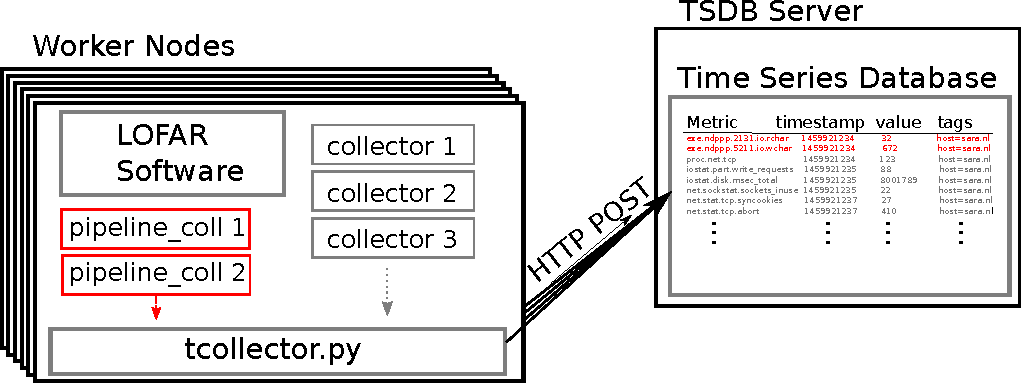
\includegraphics[width=\linewidth]{ch4/figures/figA14/TSDB_tcollector.pdf}
      \caption{Communication between worker nodes and the TSDB server, including the pipeline\_collector modules (in red). The \textit{pipeline\_collector} suite collects information on the running LOFAR pipelines, while the rest of the tcollector package collects system performance data. The existing tcollector package and its collectors are shown in gray. The collectors in gray only record metrics from the global system. }
	\label{fig:ch4_tsdb_tcollector}
\end{figure}

\subsection{The pipeline\_collector suite}\label{sec:ch4_customcollectors}



The tcollector package cannot collect data on individual processes, nor can it associate these processes with specific steps of a data processing pipeline. We've supplemented the software with the \textit{pipeline\_collector} suite\footnote{Located at https://gitlab.com/apmechev/procfs\_tcollector.git} using an executable that monitors a pipeline's running processes\footnote{Located at https://github.com/apmechev/procfsamp}. When an executable that is part of the LOFAR pipeline launches, a dedicated collector begins reporting information on the individual process. Every time a new processing step starts, the \textit{prefactor} pipeline records the step name in a log file. \textit{pipeline\_collector} determines the current running step using this log. Running the LOFAR processing concurrently with the tcollector package gives us per-step performance data without changing or slowing down the LOFAR \textit{prefactor} pipeline. Furthermore, \textit{pipelie\_collector} can be integrated with any processing pipeline as long as each pipeline step's name is recorded at its launch. 

The \textit{pipeline\_collector} suite sends data to the time series database in the same format as the rest of the collectors included in the tcollector package. 

\subsection{Setting up for future pipelines}

The setup options for \textit{pipeline\_collector} are stored in a configuration file in the root directory of the package. This file holds the sample interval, executables to monitor and the location where \textit{pipeline\_collector} can read the current pipeline step

The \textit{pipeline\_collector} suite reads the current pipeline step from a file, the location of which is specified in the configuration. This file needs to be updated each time the pipeline begins a new step. For LOFAR we have a script running with the pipeline, and determining the current step using the pipeline logs. As each pipeline has a unique sequence of steps, the current step needs to be recorded in a file in order for \textit{pipeline\_collector} to report it to the time series database. The location of the file recording the current pipeline step is read from the configuration file. 

Next, the names of the specific processes need to be included in the configuration file. In the case of LOFAR, we select the \texttt{NDPPP}, \texttt{bbs-reducer} and \texttt{losoto} processes. The \textit{pipeline\_collector} searches the running processes for the current user for these process names and launches a collector for each new process launched by the current step. 
\end{subappendices}


\section*{Acknowledgments}
APM would like to acknowledge the support from the NWO/DOME/IBM programme ``Big Bang Big Data: Innovating ICT as a Driver For Astronomy'', project \#628.002.001.

HJR gratefully acknowledge support from the European Research Council under the European Unions Seventh Framework Programme (FP/2007-2013)/ERC Advanced Grant NEWCLUSTERS- 321271.

JBRO acknowledges financial support from NWO Top LOFAR-CRRL project, project No. 614.001.351. 


This work was carried out on the Dutch national e-infrastructure with the support of SURF
Cooperative through grant e-infra 160022 \& 160152.

%\bibliography{bibliography}

%%\end{document}

%%
%% End of file `elsarticle-template-1-num.tex'.

%%%%%%%%%%%%%%%%%%%%%%%%%%%%%%%%%%%%%%%%%%%%%%%%%%%%%%%%%%%%%%%%%%%%%%%%%%%%%%%%
%2345678901234567890123456789012345678901234567890123456789012345678901234567890
%        1         2         3         4         5         6         7         8

% %\documentclass[letterpaper, 10 pt, conference]{IEEEtran}  % Comment this line out
% %                                                          % if you need a4paper
% %%\documentclass[a4paper, 10pt, conference]{ieeeconf}      % Use this line for a4
% %                                                          % paper
% %
% %\IEEEoverridecommandlockouts                              % This command is only
% %                                                          % needed if you want to
% %                                                          % use the \thanks command
% %\newcommand\Mark[1]{\textsuperscript{#1}}
% %
% %
% %%\overrideIEEEmargins
% %% See the \addtolength command later in the file to balance the column lengths
% %% on the last page of the document
% %
% %
% %%%%%%%REMOVE FOR FINAL VERSION
% %\usepackage[switch]{lineno} 
% %\linenumbers
% %%%%%%%%%%%%%
% %
% %\usepackage{lettrine}
% %
% %% The following packages can be found on http:\\www.ctan.org
% %\usepackage{graphicx} % for pdf, bitmapped graphics files
% %\usepackage{url}
% %\usepackage{cite}
% %%\usepackage{epsfig} % for postscript graphics files
% %%\usepackage{mathptmx} % assumes new font selection scheme installed
% %%\usepackage{times} % assumes new font selection scheme installed
% %%\usepackage{amsmath} % assumes amsmath package installed
% %%\usepackage{amssymb}  % assumes amsmath package installed
% %

\chapter{Fast and Reproducible LOFAR Workflows with AGLOW}\label{ch:AGLOW}
\addtitlethumb{Frontmatter}{\huge 5}{white}{gray}                                                                                           

% %  {\normalfont\large 
% %  A.P. Mechev\Mark{a,1},J.B.R Oonk\Mark{a,b,c,2}, T. Shimwell\Mark{b,3}, A. Plaat\Mark{d,4}, H.T. Intema\Mark{a,5}, H.J.A. R\"{o}ttgering\Mark{a,6}
% %  }\\[-1.5ex]

%\setcounter{footnote}{0}                                                                                                                                    

% \author{A.P. Mechev $^{1}$ and A. Plaat$^{2}$

% %\thanks{*This work was not supported by any organization}% <-this % stops a space
% $^{1}$Leiden Observatory
% 		Leiden University, 	Niels Bohrweg 2 NL-2333 CA,
%         Leiden        {\tt\small research at apmechev.com} \\
% $^{2}$Leiden Institute for Advanced Computer Science
% 		Leiden University, 	Niels Bohrweg 2 NL-2333 CA,
%         Leiden          {\tt\small a.plaat at liacs.leidenuniv.nl}%

% }
% %
% %\author{
% %
% %\IEEEauthorblockA{%
% %        \Mark{a}Leiden Observatory,\\
% %        Leiden University,\\
% %        Niels Bohrweg 2 NL-2333 CA\\
% %        Netherlands \\
% %       \Mark{1}apmechev at strw.leidenuniv.nl \\
% %       \Mark{2}oonk at strw.leidenuniv.nl \\
% %       \Mark{5}intema at strw.leidenuniv.nl \\
% %       \Mark{6}rottgering at strw.leidenuniv.nl \\
% %    }  \and
% %
% %\IEEEauthorblockA{%
% %        \Mark{b}ASTRON,\\
% %        Oude Hoogeveensedijk 4,\\
% %       7991 PD Dwingeloo\\
% %        Netherlands\\
% %        \Mark{3}shimwell at astron.nl
% %    } \and
% %\IEEEauthorblockA{%
% %        \Mark{c}SURFsara\\
% %        P.O. Box 94613\\
% %        1090 GP Amsterdam\\
% %        Netherlands\\   
% %        }  \and
% %\IEEEauthorblockA{%
% %        \Mark{d}LIACS,\\
% %        Leiden University,\\
% %        Niels Bohrweg 1 NL-2333 CA\\
% %        Netherlands\\
% %        \Mark{4}a.plaat at liacs.leidenuniv.nl
% %    }
% %}
% %
% %\usepackage[perpage]{footmisc}
% %\begin{document}



%\maketitle
%\thispagestyle{empty}
%\pagestyle{empty}


\begin{frshaded*}
    The contents of this chapter are based on a manuscript Published at the IEEE e-Science conference 2018
\end{frshaded*}
%

%%%%%%%%%%%%%%%%%%%%%%%%%%%%%%%%%%%%%%%%%%%%%%%%%%%%%%%%%%%%%%%%%%%%%%%%%%%%%%%%
\setlength\FrameRule{1.5pt}
\begin{frshaded*}
    \textbf{Original Abstract:}

The LOFAR radio telescope creates petabytes of data per year. This data is important for many scientific projects. The data needs to be efficiently processed within the time span of these projects in order to maximize the scientific impact. We present a workflow orchestration system that integrates LOFAR processing with a distributed computing platform. The system is named Automated Grid-enabled LOFAR Workflows (AGLOW). AGLOW makes it fast and easy to develop, test and deploy complex LOFAR workflows, and to accelerate them on a distributed cluster architecture. AGLOW reduces the setup time of complex workflows: typically, from months to days. We lay out two case studies that process the data from the LOFAR Surveys Key Science Project. We have implemented these into the AGLOW environment. We also describe the capabilities of AGLOW, paving the way for use by other LOFAR science cases. In the future, AGLOW will automatically produce multiple science products from a single data set, serving several of the LOFAR Key Science Projects.
\end{frshaded*}
%Target:  IEEE International Conference On e-Science
%Keywords: Workflow management software, Radio Astronomy, Distributed Computing, Big Data applications
%\end{abstract}
%
%
%%%%%%%%%%%%%%%%%%%%%%%%%%%%%%%%%%%%%%%%%%%%%%%%%%%%%%%%%%%%%%%%%%%%%%%%%%%%%%%%
%renewcommand{\thefootnote}{\fnsymbol{footnote}}
\section{Introduction}\label{sec:ch5_intro}

Data sets in radio astronomy have increased 1000-fold over the past decade\cite{sabater_datasize}. It is no longer feasible to move, store and process these data sizes at university clusters, nor to process these data manually. LOFAR, the Low-Frequency Array\cite{LOFAR} is a modern and powerful radio telescope that creates more than 5 Petabytes of data per year. At present, the majority of LOFAR time is allocated to several Key Science Projects (KSPs)\cite{lotss}. These projects need to process hundreds or thousands of observations. Typical observations produce approximately 14 TB of archived data. Obtaining high fidelity images from this data requires complex processing steps. To manage and automate the data processing, workflow management software is needed. This software needs to accelerate LOFAR processing on a High Throughput Computing (HTC) cluster while ensuring it is easy to prototype, test, and integrate future algorithms and pipelines. 
	
To automate LOFAR data processing, we have worked with the LOFAR Surveys KSP (SKSP). Together, we designed a software suite that integrates LOFAR software\cite{cookbook} with the Dutch grid infrastructure\cite{dutchinfra}. This software, based on Apache Airflow\footnote{\url{https://airflow.apache.org/}}, makes it easy to add future science cases, extend and modify pipelines, include data quality checks, and rapidly prototype complex pipelines.  For the SKSP use cases, AGLOW achieves a significant reduction in development time: from months to days, allowing researchers to concentrate on data analysis rather than management of processing.  Additionally, and perhaps more importantly, the software versions and repositories used are defined within the workflow. This makes reproducibility an integral part of the AGLOW software.  Finally, the software is built to  leverage an HTC cluster by seamlessly submitting the processing jobs through the cluster's job submission system\cite{glite}. The work presented here builds on our previous work parallelizing single LOFAR jobs\cite{mechev} on a distributed environment. The majority of processing was done at SURFsara at the Amsterdam Science Park\cite{SurfSara}, which is one of the sites used by the LOFAR Long Term Archive (LTA)\footnote{\url{https://lta.lofar.eu}}. Ongoing efforts include scheduling and processing data at clusters in Pozna\`{n} in Poland and J\"{u}lich in Germany. 

\textbf{Contributions:}
The main features of the AGLOW software are the following:
\begin{itemize}
\item Integration of the Grid middleware with Apache Airflow, allowing us to dynamically define, create, submit and monitor jobs on the Dutch national e-infrastructure.
\item Integration of the LOFAR (LTA) utilities in  Airflow, facilitating pipeline developers to automate staging (moving from tape to disk) and retrieval of LOFAR data.
\item Integration of the SURFsara storage with Airflow, making LOFAR pipelines aware of the storage layer available at the Dutch national e-infrastructure.  
\item Ease of creating simple software blocks, with which users can integrate and test their pipelines. 
\item Storing all software versions and script repositories as part of the workflow to make LOFAR processing reproducible and portable. 
\end{itemize}

\textbf{Outline:}
The organization of this manuscript is as follows: We provide background on data processing in radio astronomy and why LOFAR science requires complex workflows and cover workflow management algorithms and capabilities (section \ref{sec:background}). We discuss related work in workflow management (section \ref{sec:related}). In section \ref{sec:AGLOW}, we introduce our software and two use cases. Both of our use cases require acceleration at an HTC cluster and automation by a workflow orchestration software. We follow these examples with details on the integration between LOFAR software, LOFAR data and the resources at SURFsara in Amsterdam in section \ref{sec:extending}. Finally, we discuss our results (sect. \ref{sec:results}) and look ahead to the demands of future LOFAR projects and upcoming telescopes in section \ref{sec:conclusions}. 

\section{Background}\label{sec:background}

This work lies at the intersection of Radio Astronomy and Computer Science. The goal of the study is to leverage the flexibility of an industry standard workflow management software and use CERN's Worldwide Computing Grid\footnote{\url{http://wlcg.web.cern.ch/}} at SURFsara \cite{grid} to accelerate reproducible processing of LOFAR data. 


A single LOFAR surveys observation is recorded in distinct frequency chunks (henceforth called `Subbands'), each of which is uploaded to the LTA as a separate file. Some of the processing steps require the entire frequency information, while other steps can run independently and operate on a single Subband. The latter steps can be easily accelerated on an HTC cluster by taking advantage of the data level parallelism. 

Multiple scientific projects may desire to run different processing steps on a single LOFAR observation. To minimize time spent on retrieving data from the LTA and eliminate re-processing of data, pipelines for multiple science cases need to be integrated together. This integration should be done by a software that encodes the dependencies between different steps and automatically executes processing steps once their dependencies have been met. Software packages that solve these challenges are called `workflow management software' (see, e.g., \cite{workflow1,workflow2,workflow3}.)

\section{Related Work}\label{sec:related}

A workflow is described by a set of tasks. The dependencies between these tasks are encoded in a Directed Acyclic Graph (DAG) \cite{dag}. This data structure imposes a strict dependency hierarchy between the tasks \cite{dagalgos}. This means that there exists a well-defined execution order and a well-defined list of dependencies for each task. The execution order is typically determined by algorithms such as Kahn's algorithm \cite{Kahn} or a depth-first search \cite{dfs}.

Workflow management software is used in various fields from research to industry. In biology, gene sequencing and analysis pipelines require automation of multiple processing steps. In gene sequencing, Toil\footnote{\url{https://toil.readthedocs.io}} has been successfully used to automate RNA sequence analysis\cite{toil}. Additionally, many  software teams in biotech develop their own in-house workflow management software \cite{nextflow}.  


Currently, we can parallelize a single processing step of the pipeline using the Grid LOFAR Tools (GRID\_LRT\footnote{\url{https://github.com/apmechev/GRID_LRT}}) \cite{mechev}. The LOFAR Surveys science cases incorporate multiple steps with inter-linked dependencies. Resolving these dependencies can be done efficiently by a comprehensive workflow orchestration software. The purpose of such software is to resolve dependencies between the multiple tasks in a workflow, execute these tasks, and track the status, logs, output, and run time of each task. 

In astronomy, workflow systems have been developed that are telescope specific, such as ESOReflex\cite{reflex} by the European Southern Observatory. Other projects, such as astrogrid\footnote{http://www.astrogrid.org} and 'Workflow 4Ever'\footnote{http://wf4ever.github.io/ro/}, have either been completed or are no longer supported. The astrogrid project, for example, was a collaboration to create standards, infrastructure, and software for distributed astronomical processing. Its operation phase spanned 2008-2010. Workflow4Ever, likewise, has been out of support since 2013. To ensure continuing support for the LOFAR workflows, we have decided to use a leading enterprise workflow management software, Airflow.

Airflow is an open source Python software package developed by Airbnb\footnote{\url{https://www.airbnb.com/}} to manage complex workflows. It encodes workflows in Python files and makes it easy to re-use, re-arrange, schedule and execute blocks in a user-defined workflow. Airflow is capable of scheduling and executing workflows by resolving the dependencies between tasks and scheduling these tasks for execution. The software uses a metadata database\footnote{In our case implemented by Postgresql} to retain metadata such as task state, execution date, and output. While Airflow allows building workflows easily from Python and bash functions, it can easily be extended to support custom processing scenarios. Additionally, Airflow conforms to the Common Workflow Language (CWL) \cite{cwl} standard using the \textit{cwl-airflow} package \cite{cwlairflow}, meaning it can execute CWL workflows as well. Finally, Airflow is part of the Apache incubator and upon certification will receive continual support by the Apache software foundation\footnote{https://www.apache.org/}. 


\section{AGLOW}\label{sec:AGLOW}

Complex astronomical pipelines are time consuming to develop and operate. Furthermore, they may evolve rapidly to incorporate new processing techniques or requirements. Migrating these pipelines to a distributed, high throughput environment is often justified, or even required, in order to meet the timelines set by scientific projects. The time saved by running on a cluster must be balanced by the flexibility and development time required to implement or update the scientific pipelines. To address these concerns, we have developed a software package, Automated Grid-enabled LOFAR Workflows (AGLOW)\footnote{\url{https://github.com/apmechev/AGLOW}}. AGLOW is based on Airflow and the LOFAR software and addresses issues with automation and acceleration of LOFAR processing. 

With AGLOW, we can translate LOFAR pipelines into DAGs. We provide the tools that enable users to easily implement LOFAR science pipelines and execute them on a distributed architecture. Using these tools, the data processing required by various LOFAR science cases is automated and accelerated. 

\subsection{AGLOW: Case Study}

For our case-study, we have chosen two ways to process LOFAR Surveys data: coverage and depth. The Surveys Key Science Project (SKSP)\cite{lotss} is an ambitious project to map the northern sky at low frequencies using the Dutch LOFAR stations. These maps will help understand the formation and evolution of massive black holes, galaxies, clusters of galaxies and large-scale structure of the Universe.  

The LOFAR surveys observations consist of several tiers with the widest Tier (Tier 1) covering the whole sky visible from the Northern Hemisphere with 3168 observations of 8 hours each \cite{lotss}. The other tiers (Tier 2, Tier 3) consist of much longer observations of smaller sections of the sky and can collect hundreds of hours of data for a single  direction. The deepest single field being analyzed, in collaboration with the EoR group, is the North Celestial Pole (NCP) field which has $\sim$1700 hrs of observations to date.  Processing this data will create an image with an unprecedented resolution and sensitivity. Here we have implemented processing pipelines for both the Tier 1 data and Tier 2 data into AGLOW. 

The scientific importance of these two examples, as well as the large processing requirements, make them ideal candidates for acceleration and automation with AGLOW.

\subsubsection{Surveys Project: All Sky Survey}\label{sec:coverage}

The main driver for the development of AGLOW and its constituent packages has been the LOFAR SKSP Project. A typical 8-hour observation produces 14 TB of data. This data is eventually reduced to several hundred gigabytes. Data needs to be processed by two pipelines: first by the Direction Independent (DI) pipeline, and then by the Direction Dependent (DD) pipeline. 

We have split the DI pipeline into four stages, and the DD pipeline into two subsequent stages. Splitting up the pipelines in stages allows speedup through parallelization for the stages that can benefit from data-level parallelism. Additionally, this setup allows fault tolerance and easy re-processing.Importantly, with AGLOW, adding new functionality to the pipeline is easy and can be done at any time without disrupting current processing. Current SKSP processing is easily started by launching a new DAG-run in Airflow. We schedule these runs daily at midnight, however they can also be started manually bu users. 

\subsubsection{Deeper Surveys Fields}

To create deep images of a single field, minor modifications were made to the processing pipeline described in the previous section. Scripts were included to re-align the data in the frequency axis, and the DD processing steps include an extra final combination step that stacks multiple observations. Being able to rapidly test alternative processing strategies is crucial to creating a deep image of the NCP field. With the success of this project, future deep LOFAR observations will be processed with these pipelines.

\subsection{AGLOW: Implementation}\label{sec:implementation}

AGLOW combines the LOFAR software, the Grid LOFAR Tools (GRID\_LRT), and Airflow to allow automation and makes large-scale LOFAR processing easily reproducible. The components of the AGLOW software are shown in Fig. \ref{AGLOW_structure}.  In this section, we will discuss these components and their functions. 

\begin{figure}[thpb]
 \centering
  \framebox{\parbox{3.3in}{      
  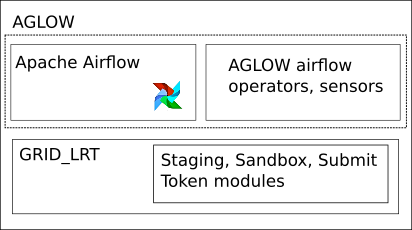
\includegraphics[width=0.45\textwidth]{ch5/figures/AGLOW_structure.png}
 }}
    \caption[Design of the AGLOW software, including its constituent packages.]{Design of the AGLOW software, incorporating Airflow, the GRID\_LRT package\cite{mechev} and custom operators designed to integrate LOFAR software, Grid middleware and dCache storage. GRID\_LRT is a software package developed to parallelize single LOFAR jobs at SURFsara. It contains several modules to help set up, and launch jobs on an HTC cluster at SURFsara. Airflow is a stand-alone package by Airbnb, which is extended with several classes that couple Airflow with the Grid infrastructure. These classes are collectively named the AGLOW operators/sensors. }
 \label{AGLOW_structure}
\end{figure}


\subsubsection{GRID LOFAR Tools and LOFAR software}
We have previously developed tools to create LOFAR jobs and launch them on a distributed infrastructure\cite{mechev}. These tools have matured to a point where it is easy to both plug and play existing scripts and extend the framework to add more complex pipelines. These steps make it possible for a user to batch execute bash or Python scripts on their LOFAR data in parallel. After the scripts are executed, the results are uploaded to shared dCache storage\cite{dcache} at SURFsara\cite{SurfSara}. 

More complex steps use additional Github repositories, such as the prefactor\footnote{https://github.com/lofar-astron/prefactor} for direction independent calibration or DDF-pipeline\footnotemark{}  for direction-dependent calibration and imaging. The sequence of steps is encoded in parameter-set files (parsets), which can be modified and dropped into AGLOW depending on the processing requirements. Users have full control over which git repository, branch and commit number to use for each processing step. 

With AGLOW, we can easily include the DDF-pipeline and prefactor repositories, as well as any other scripts. Since these scripts are tracked by git \cite{torvalds2010git}, a full commit and branch history of the scripts is available. We use this history to make processing reproducible, by using the same git-commit for all LOFAR data sets. 

In addition to these script repositories, we have integrated the most common software packages used to process LOFAR data with AGLOW. These are the Default Pre-Processing Pipeline (DPPP)\cite{cookbook}, the LOFAR Solutions Tool (LoSoTo), WSclean \cite{wsclean}, AOflagger\cite{aoflag}, CASA\cite{casa}, pyBDSF\cite{bdsf}, DDFacet\cite{tasseDDFacet} and KillMS\cite{smirnov_tasse_KillMS,tassekalman}.

\footnotetext{https://github.com/mhardcastle/ddf-pipeline. DDF-pipeline is a leading example of a Direction Dependent calibration pipeline used for LOFAR data. It uses DDFacet \cite{tasseDDFacet}, KillMS \cite{smirnov_tasse_KillMS} and to create high quality images. }

\subsubsection{Extending Airflow}\label{sec:extending}

Two types of modifications were made to Airflow to allow processing on a Grid environment. First, functions were added to check the number of files located in intermediate grid storage. We use this to decide whether to stage files, or whether enough files have been successfully processed by a previous task. 

Second, more complex tasks were implemented as Airflow operators or sensors (Figure \ref{AGLOW_Operators}). These tasks include creating job description files, setting up job scripts, launching jobs using the gLite workload management system and monitoring the status of these jobs. Future additions will include operators that evaluate the current cluster workload and make decisions on location to launch the data processing. With the AGLOW package, such tasks are easy to implement without modifying or interrupting processing. This leads to an easily reproducible, intelligent scientific processing that is also efficiently executed and requires minimal interaction. The operators and sensors added to Airflow are shown in Fig. \ref{AGLOW_Operators}. The most commonly used ones are described below:

\paragraph{Staging}
AGLOW stages data through the ASTRON staging API, which is made available through the GRID\_LRT software \footnote{\url{https://grid-lrt.readthedocs.io/en/latest/staging.html\#grid-lrt-staging-stage-all-lta}}.This API loads the user's LTA credentials from a file. Using these credentials, AGLOW stages the required files at the respective LTA site. The AGLOW staging operator waits until all the files have been staged before returning a successful exit status. 

\paragraph{Sandbox}
Scripts to retrieve, process and upload the data are stored in a sandbox, as described in \cite{mechev}. The LRT\_Sandbox operator that builds this sandbox directly uses the GRID\_LRT Sandbox module to build and upload the sandbox according to the user-provided configuration file. 

\paragraph{Token Creation}
Jobs parallelized with GRID\_LRT store processing parameters inside CouchDB documents called PiCaS Tokens. Each token corresponds to one grid processing job. These tokens are created by the LRT\_Token operator in AGLOW. This operator uses the GRID\_LRT Token module to define tokens and create them from a list of links to LOFAR data. 

\paragraph{Job Submission}
The job submission at SURFsara is done through the GRID\_LRT submit module. This module is a python interface to the glite job submission system. It is wrapped in the glite-submit operator in AGLOW, which returns the ID number of the job. AGLOW includes a gliteSensor, which uses this ID to wait until all the processing jobs have finished. 


Using AGLOW to accelerate the execution of a pipeline requires deciding how to split the processing to benefit from parallelization. Once the steps to be parallelized are selected, users can add git repositories of scripts to the configuration file. Next, each step is added to a Python script called the DAG file. This file is placed in the Airflow's dags folder, which adds it to AGLOW. An example DAG file can be found at \url{https://aglow.readthedocs.io/en/latest/dags.html}. Users who want to implement a new workflow design the DAG files and add them to Airflow's dags folder. Workflows are migrated to a new server, by transferring the DAG and configuration files to the new AGLOW instance. 


\begin{figure}[thpb]
 \centering
  \framebox{\parbox{3.3in}{      
  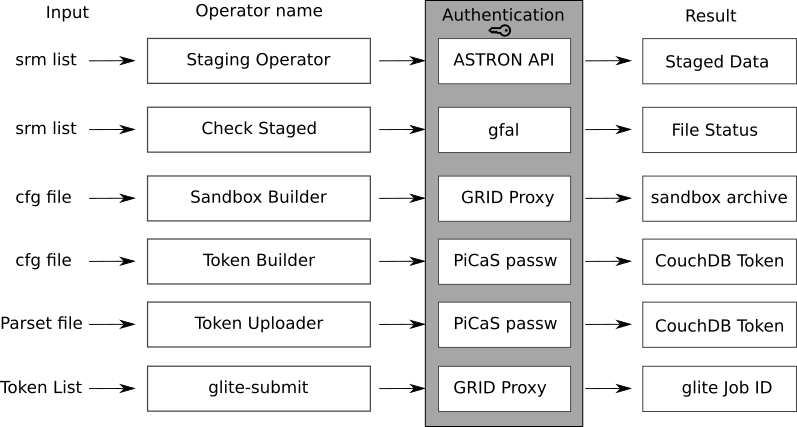
\includegraphics[width=0.45\textwidth]{ch5/figures/Operators.png}
 }}
    \caption[Graphical representation of the Airflow Operators built for AGLOW]{Airflow Operators for Staging LOFAR data, creating job descriptions and submitting jobs to the Dutch grid. On the left is the input given to each operator. `SRM lists' are lists of links to data at the LOFAR LTA or located on the SURFsara dCache storage. Parsets are files specific to `prefactor' and `DDF-pipeline' and define the processing for each pipeline step. Finally, the `Sandbox' and `Token' operators read their parameters from a configuration file. The use of a scripts sandbox and job description tokens is detailed in our previous work\cite{mechev}. Documentation of the operators is available at  \protect\url{https://aglow.readthedocs.io/en/latest/operators.html}}
 \label{AGLOW_Operators}
\end{figure}
 

\subsection{AGLOW: Jobs}

Once LOFAR observations are downloaded from the LTA, they are typically processed with several packages before producing a science ready data set. We have integrated these packages with Airflow to make it easy to create complex LOFAR workflows. 

Each of the processing steps above requires extra set-up to process on the Dutch Grid infrastructure. The job scripts setup, job description, and job submission are done by the GRID\_LRT package\cite{mechev}. With AGLOW, we automate this setup, enabling users to focus on developing more comprehensive data processing pipelines. Below we outline several possible steps a user can use in their pipeline. 

\subsubsection{DPPP Parset}
The DPPP software is used extensively in LOFAR data processing. It has many capabilities such as flagging bad data, averaging data in time and frequency, and calibrating the data with a sky-model. 

The input parameters of this software are stored in a text file called a parset. The input data and the DPPP parset are sufficient to define a DPPP execution step. As noted in section \ref{sec:background}, LOFAR data is split in frequency into Subbands. Much of the DPPP processing, such as averaging and flagging, can be done independently for each Subband, thus they can be processed on independent machines. This parallelization makes these steps a perfect candidate for an HTC cluster. For a data set that is split into 244 Subbands, 244 jobs are launched concurrently. 

In Airflow, the DPPP parset task is encoded in a DAG (Fig. \ref{fig:NDPPP_DAG}). The DPPP DAG is a linear workflow that consists of the 'sandbox' setup, creation of the job-description documents, uploading of the DPPP parset and job launching and monitoring.


\begin{figure}[H]
 \centering
 \framebox{\parbox{2.5in}{      
  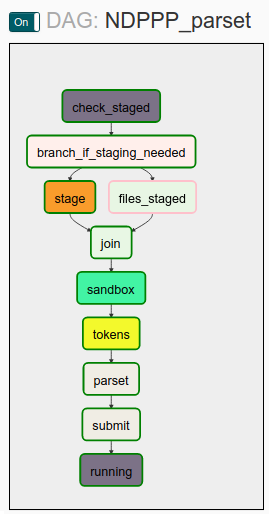
\includegraphics[width=0.35\textwidth]{ch5/figures/NDPPP_DAG.png}
 }}
    \caption[Renderng of the DAG encoding a DPPP parset as shown by the Airflow User Interface.]{Render of the DPPP parset DAG in the Airflow User Interface. This view shows the setup and submission steps. Even this simple DAG can include branching options such as the \texttt{branch\_if\_staging\_needed} task which checks if the data is not staged and stages it. All of the operators in this figure are part of the AGLOW software. Their inputs and outputs are shown in Fig. \ref{AGLOW_Operators}. Using configuration files, the NDPPP DAG can be used by different users for different science cases making it portable and maintainable. These features make reproducible science with LOFAR data easy. 
 }
 \label{fig:NDPPP_DAG}
\end{figure}

\subsubsection{WSclean Job}

The WSclean\cite{wsclean} package is used to create an image from a LOFAR data set. This software has a very wide range of parameters options, however, it cannot take a parset file as an input. Instead, the parameters are specified in the command line. In the AGLOW implementation, we parse all the command-line parameters from a text file, referred to as the 'wsclean parset'. This file is added to the jobs in the same way as the DPPP parset, i.e. using the \textit{Token Uploader} Operator. The DAG for the wsclean software uses the same blocks as the DPPP DAG, with different configuration and parset files. The reuse of Airflow operators makes maintainability of all tasks easier. 

\subsection{Shell/Python Script}

Users that require the run of multiple software packages on a single data set can craft a custom shell or Python script that executes these steps using the LOFAR tools during a single distributed job. This option increases flexibility and minimizes the overhead associated with scheduling and running multiple jobs in sequence. At the workflow orchestration level, we use the same Airflow operators as the above tasks. The script is uploaded to the job description database using the \textit{Token Uploader} Operator. It is executed once the jobs are launched. 

Currently only the LOFAR Spectroscopy project uses custom shell scripts to process LOFAR data. A recent study of carbon recombination lines used a custom bash script to calibrate and image LOFAR data on the SURFsara \texttt{GINA}\footnote{The \texttt{GINA} cluster is an HTC cluster located at SURFsara integrated with the Dutch Grid initiative. It supports massively parallel processing which is required to efficiently process LOFAR data with \textit{prefactor}. } cluster \cite{pedro}. 

\subsection{Prefactor parset}

The input to the prefactor pipeline software is a parset file which describes a linear workflow. The description of this workflow consists of a list of processing steps and their associated parameters. The `prefactor' package uses the LOFAR software to do the direction-independent calibration of the archived LOFAR datasets. Prefactor steps are executed by the generic pipeline framework\cite{cookbook}. While this framework can run a sequential pipeline, it is not capable of conditional branching nor parallelization on all cluster architectures. The original goal of the GRID\_LRT software was to tackle the parallelization challenge while AGLOW solves the additional challenge of pipeline management. 

We have already processed more than 50 datasets through the `prefactor' DAG using AGLOW. The full `prefactor' pipeline is shown in figure \ref{SKSP_workflow}. This DAG shows the four processing steps as well as additional Python operators that manage the staging and result verification. 

\subsection{DDF-pipeline}

The final AGLOW DAG is the implementation of the DDF-pipeline repository which is a pipeline that is extensively used by the LOFAR surveys KSP and is described in detail in \cite{lotss}. This pipeline operates on the products of the prefactor pipeline and consists of a series of calibration and imaging loops with the objective of creating a final science quality image. For each of these loops the majority of the processing time is spent in DDFacet\cite{tasseDDFacet} and KillMS\cite{smirnov_tasse_KillMS,tassekalman} steps that perform the direction-dependent imaging and calibration respectively. 

In total, DDF-pipeline takes $\sim$4\, days of processing to complete. As DDF-pipeline creates large intermediate files we have so far not divided the pipeline into too many steps to avoid filling the storage on the \texttt{GINA} cluster. However, we have split the pipeline into two steps and there is further potential for parallelization that will be implemented in the future. 

\subsection{Linking Multiple Jobs}

Pre-processing of LOFAR SKSP data can be done by a single DPPP task, with 244 jobs running in parallel. More complex LOFAR pipelines will include multiple processing tasks as well as tasks responsible for job setup. Therefore, it is important to facilitate running multi-step pipelines with AGLOW. 

Creating workflows by defining dependencies between tasks is a core Airflow capability. We use this functionality to link multiple steps of a LOFAR pipeline together. In the SKSP pipeline, we take advantage of the data level parallelism for the initial processing steps for the calibrator and target. The other two  steps are run as a single grid job. Switching the parallelization for each step is done by changing the number of datasets per node parameter in the configuration file for each step. 

\section{Results and Discussions}\label{sec:results}

The implementation of AGLOW makes it possible to efficiently process LOFAR data with minimal user interaction. The scheduling algorithm automatically launches pipelines, meaning that there is little time spent between runs. Additionally, controlling/fixing the version of the scripts is done by specifying the commit of each script repository. This makes data processing easily reproducible. Once the dependencies of multiple science pipelines have been encoded in a DAG, Airflow efficiently executes this DAG, running tasks in parallel where possible. 

An important feature of AGLOW is the loose coupling between pipeline logic, software versions, pipeline parameters, and datasets. The goal of this decoupling is to give users complete control over all the processing variables. With AGLOW, one can develop the pipeline logic independently of the LOFAR software versions and conversely update the LOFAR software and script repositories independently from the pipeline logic. Finally, the Airflow operators are themselves decoupled from the scientific pipelines. As these operators are reused, this decoupling makes them easy to maintain and extend.

The first LOFAR processing pipeline integrated with AGLOW was a single linear workflow, with only one submission to the compute cluster. This workflow is used to reduce the data size making data retrieval to research institutes less time consuming. We offer this workflow as a service to LOFAR users who do not have a high-bandwidth connection to the LOFAR Archive. 

A more complex pipeline was implemented: the LOFAR direction independent calibration pipeline (`prefactor'). The scientific importance and complexity of this pipeline make it a good case study for the capabilities of the AGLOW software. We show that AGLOW's design allows integration of more complex data processing workflows with the Dutch Grid resources. These workflows can be either used by PIs of LOFAR projects or offered as a processing service to the wider astronomical community. Since March 2018, more than 300 `pre-factor' datasets have been processed with  the SKSP workflow. With AGLOW, we have been able to process data with an average cadence of 50 observations per month. 

In large part thanks to their flexibility, automation, and Grid integration, AGLOW and GRID\_LRT have become a standard part of the Direction Independent processing for the LOFAR SKSP project. 


\section{Conclusions}\label{sec:conclusions}

In this work, we have detailed a comprehensive workflow management software for processing radio astronomy data on a distributed infrastructure. We leverage an industry standard workflow management software, Airflow. Using its capabilities, we make it possible to build, test, automate and deploy LOFAR pipelines on short timescales, generally from months to days. With the flexibility of Airflow's Python and Bash operators, users can design their own workflows, as well as co-ordinate more complex science cases. In this way, AGLOW facilitates reproducible processing of scientific data. In the future, AGLOW will support additional LOFAR science cases including Long Baselines and Spectroscopy. In this article, we have described our implementation of the data processing pipelines used by the LOFAR Surveys Key Science Project. 

Future work includes further de-coupling of the Grid-setup and pipeline logic. We will do this by creating `sub-dags' (details in \ref{sec:Subdags}) for each type of LOFAR jobs. Using these sub-dags will reduce the complexity of scientific workflows while also making the code even more reusable and thus easier to maintain and upgrade. Efforts to integrate processing at the other two LTA sites, (J\"{u}lich and Pozna\'{n}) have already started with `prefactor' runs being performed on J\"{u}lich using a modified version of the SKSP workflow. The software also currently works on the Eagle cluster at Pozna\'{n}. Combining the J\"{u}lich and SURFsara workflows will be done in the future so that AGLOW can track and start processing at multiple clusters. 

Finally, AGLOW can be used as a `LOFAR As A Service' model.  In this model, users only provide an observation ID and processing parameters and receive the final results upon job completion. This model will build upon previous success offering LOFAR processing to users without login to the \texttt{GINA} cluster \cite{oonk_prep}. This previous work was already useful for studying radio absorption in Cassiopeia A \cite{maria} and a `data-to-images' service will be valuable to the whole LOFAR community.

Our experience with automating LOFAR scientific workflows on a distributed architecture will be valuable when setting up data processing for future Radio Telescopes such as the Square Kilometer Array \cite{ska} . 


%\addtolength{\textheight}{-12cm}   % This command serves to balance the column lengths
                                  % on the last page of the document manually. It shortens
                                  % the textheight of the last page by a suitable amount.
                                  % This command does not take effect until the next page
                                  % so it should come on the page before the last. Make
                                  % sure that you do not shorten the textheight too much.

%%%%%%%%%%%%%%%%%%%%%%%%%%%%%%%%%%%%%%%%%%%%%%%%%%%%%%%%%%%%%%%%%%%%%%%%%%%%%%%%



%%%%%%%%%%%%%%%%%%%%%%%%%%%%%%%%%%%%%%%%%%%%%%%%%%%%%%%%%%%%%%%%%%%%%%%%%%%%%%%%



%%%%%%%%%%%%%%%%%%%%%%%%%%%%%%%%%%%%%%%%%%%%%%%%%%%%%%%%%%%%%%%%%%%%%%%%%%%%%%%%
\begin{subappendices}

\section*{APPENDIX}
 
\begin{figure*}[!ht]
 \centering
 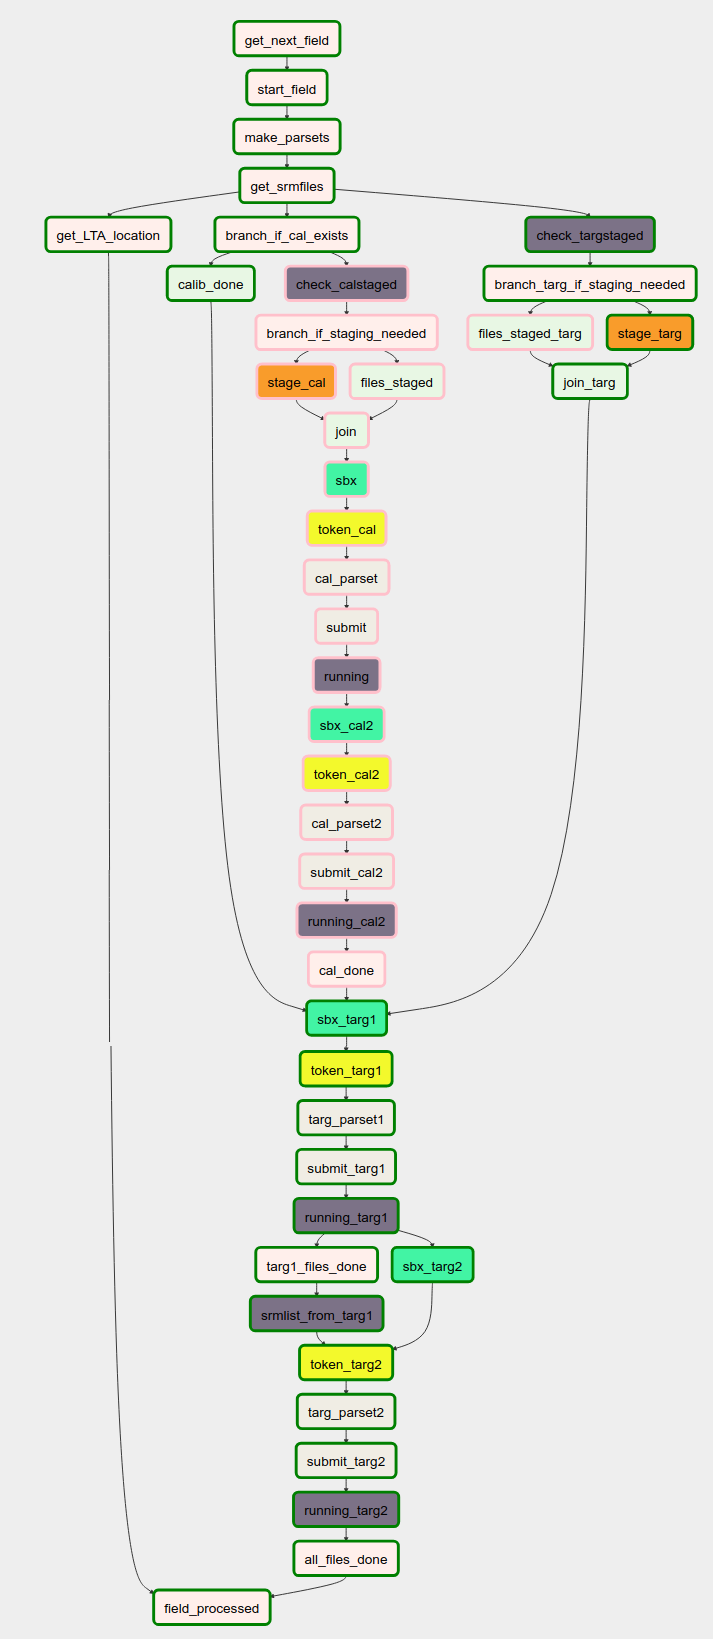
\includegraphics[width=0.52\textwidth]{ch5/figures/SKSP_Dag1.png}
    \caption[Render of the DAG encoding the full prefactor pipeline.]{Workflow for the prefactor pipeline. Here we show the reuse of AGLOW operators for the four prefactor steps. In addition to the LOFAR processing, we also have conditional operators to skip processing of the calibrator if it has been previously processed. This is done by the `branch\_if\_cal\_exists' task. We also have a final step that checks if all the results have been uploaded, done by the `all\_files\_done' task. Likewise, quality checks can be added in this workflow wherever needed.}
 \label{SKSP_workflow}
\end{figure*}

The LOFAR SKSP workflow is shown in Figure \ref{SKSP_workflow}. This figure shows how reuse of the staging, setup operators, and glite-wms sensors makes maintainability easy and allows rapid prototyping of complex pipelines. 
 
 This workflow additionally takes advantage of Airflow's \textit{PythonOperator} to check if the LOFAR data is on disk at the archive and whether all final products were uploaded by each step. AGLOW also allows for staging the calibrator and target files concurrently. When the data is staged, Airflow continues with the processing of that data. 

\subsection{Sub-DAG}\label{sec:Subdags}
Airflow allows developers to include entire DAGs as a single task in their workflow. Airflow can trigger a DAG execution based on parameters provided by the parent DAG. This feature makes it possible to concatenate short, commonly used tasks into DAGs and call them in a parent workflow. Using sub-DAGS makes the code more maintainable and easy to use, while it makes workflows simpler. For LOFAR, Sub-DAGs are used to automate job submission, making the resulting scientific workflows simpler. 

   
% Appendixes should appear before the acknowledgment.
\end{subappendices}
\section*{Acknowledgment}

APM would like to acknowledge the support from the NWO/DOME/IBM programme ``Big Bang Big Data: Innovating ICT as a Driver For Astronomy'', project \#628.002.001.

The processing and storage functionality that has made this project possible was enabled by SURF Cooperative through grant e-infra 160022 \& 160152. The LOFAR software and dedicated reduction packages
on \url{https://github.com/apmechev/GRID_LRT} were deployed on the e-infrastructure by the LOFAR e-infra group, consisting of J.B.R. Oonk (SURFsara \& Leiden Observatory), A.P. Mechev (Leiden Observatory).

This chapter is based on data obtained with the International LOFAR Telescope (ILT) under project codes LC2\_038 and LC3\_008. LOFAR (van Haarlem et al. 2013) is the Low-Frequency Array designed and constructed by ASTRON. It has observing, data processing, and data storage facilities in several countries, which are owned by various parties (each with their own funding sources), and which are collectively operated by the ILT foundation under a joint scientific policy. The ILT resources have benefited from the following recent major funding sources: CNRS-INSU, Observatoire de Paris and Universit\'{e} d’Orl\'{e}ans, France; BMBF, MIWF-NRW, MPG, Germany; Science Foundation Ireland (SFI), Department of Business, Enterprise and Innovation (DBEI), Ireland; NWO, The Netherlands; The Science and Technology Facilities Council (STFC), UK
%%%%%%%%%%%%%%%%%%%%%%%%%%%%%%%%%%%%%%%%%%%%%%%%%%%%%%%%%%%%%%%%%%%%%%%%%%%%%%%%

%\addtolength{\textheight}{-12cm}   % This command serves to balance the column lengths
% %\bibliographystyle{unsrt}
% %%%\bibliographystyle{abbrv}
% %\bibliography{bibliography}



% %\end{document}

\input{ch6/chapter6.tex}
\input{ch7/chapter7.tex}

\chapter{Conclusion}

\label{ch:conclusions}


\section{Summary of Thesis Achievements}

This work focuses on the software built to accelerate and parallelize LOFAR processing and the insights obtained into large scale processing of LOFAR data. To date, we have helped process an unprecedented 8 petabytes of data for the LOFAR Two-Meter Sky Survey (LoTSS), data which has led to  more than 30 publications. We describe a generic platform for scaling astronomical processing across multiple clusters, focused on the solutions for bulk LOFAR processing.  


\section{Applications}

While this work focuses specifically on accelerating LOFAR workflows, specificaly the \texttt{prefactor} pipeline, the software developed can be integrated with any arbitrary processing pipeline.  


\section{Future Work}

The Square Kilometer Array, (SKA) is a planned aperture synthesis radio telescope expected to have a total collecting area of one square kilometer.  

\stopthumb
\cleardoublepage
\phantomsection
\addcontentsline{toc}{chapter}{Acknowledgements}
\begin{thesisacknowledgements}

    \newcommand{\bees}[1]{\includegraphics[height=\fontcharht\font`\B]{coloremoji.sty/emoji_images/hires/#1.pdf}}

Hard to believe that it was four whole years ago that I returned to Leiden to pursue a Ph.D. at the Sterrewacht. Over these years, I was lucky to make so many colourful friends and vivid memories, all of which made the 'Winter' weather a little more bearable. I'm not sure a few short pages can summarize the beautiful people I spent my time at the Sterrewacth with, but I'll have to try nevertheless.

    First, I'd like to thank the diverse and energetic LOFAR group. Josh, who always has a new intriguing topic to discuss, and is overflowing with ambitious ideas. Jit, who is that friend that every friend needs. It's no wonder he's the go-to choice for a paranymph: he's reliable and easy going, and that's no secret! Kim and Pedro, probably the first real users of my software must be commended on their patience and goodwill. Frits, with whom we've shared too many moments complaining about software over beer (or coffee, or tea, or over messenger), I wish you best of luck with the heavy mantle of making sure our software works. Gabriella, Andrea, and Francesco, grouped together for no particular reason at all, running into you randomly (or pseudo-randomly) in Bologna was a pleasant surprise. You'd be happy to know that you'll always be associated in my mind with quality food and quality time together. Federica, Amanda, and Leah, the renouned LOFAR ladies, it is always a pleasure running into you at our conferences and workshops, both in the Netherlands and abroad. I sincerely wish you the utmost success in your careers. Carole, I had lots of fun on the many occasions we spent together. Thanks for being enthusiastic enough to join me at a beer festival just before a long week of LOFAR workshopping.

    To my slav friends, it was a pleasure squatting with you. Although we only had a couple of slav dinner nights together, they were a complete success! Matus, you have been the best neighbour and most reliable friend one could wish for. I wish you all the success, and hope we still have beers at Plantage every once in a while. Give the bunnies a hug from me! L\'ydia, thank you so much for your kind words and all the chats we had together. Andrej, you are already sorely missed in our friday borrels. Best of luck in Germany and keep on dancing! Liuba, it was pleasure sailing with a seasoned sailer as you. The stories fro your sailing trip still inspire me to one day drop everything and sail the seven seas (yarrr). Aleksandrina, it's always great seeing you at LEO events! It was you who introduced me to LEO, and it looked so fun I decided to be part of the board myself! Vanja, the dishes you bring to our slavic dinners were all exceptional! It's been lots of fun to have someone that you can practically understand in your native tongue.  Micha\l{}, \L{}ukasz, and Aleksandra, it's always a party when you're around! Thanks for bringing the Polish atmosphere with you, and of course thanks for the pierogi.

    To all borrel peeps, thanks for all our chats on Fridays! Merrel, Arthur, and Jeroen, thanks for bringing the neccessary Dutchness to our borrels. Dilovan, hope you keep channelling your inner Mallory Archer and that the future borrel committees treat you with quality wine! Mantas, keep dropping sick beats at the sterrewacht parties! Anna, u w0t m8? I'm flattered that you take me as a fashion authority, I'll pretend that I actually am. Sanjana, hope one day you are able to adopt a little duckling. Let me know if you hear about those prestigous post-docs at McDonalds, they're hard to come across I hear. Fraser, Alex, and Maaike, I'll miss having the occasional Canadian corner at our borrel.

    To the big Dipper, thanks for organizing our weekly celebration of a week well spent. I will always remember that there's a slight possibility that bees \bees{1F41D} are just mad \bees{1F621} bee\bees{1F41D}cause someone cut\bees{2702}them off in traffic\bees{1F698}\bees{1F621}\bees{1F697}\bees{1F621}\bees{1F699}\bees{1F616}\bees{1F68C}. I hope I don't turn into a bee in mid acknow--

   Our agraphia group was a fun little exercise and really helped me regiment my writing. Thanks Francisca for setting it up. It was fun doing our bi-weekly calls with you \L{}ukasz and Ylva. We made so much progress together! To all my Astronomy On Tap compatriots, it was plenty fun running the events together. Liz and Vincent, thanks for putting in all the work to organize these events, your work really made the events memorable. Fran, Carmen,  and Themiya, your hard work makes the events run smoothly. Maaike, my partner in crime, filming is always more fun when you're around. Best of luck heading the video team when I'm gone! Alex, we gotta catch another Rye and ginger at de Burcht. No Canada Dry, but we'll make do.
















    LOFAR: Reinout, Aayush, Martijn, Nicolina, Rafael
    Borrel: Marta, Kirsty
    Other STRW: Tommasso, Maria Christina, Emanuelle, Marina, Malavika, Robin, Christos, Turgay, Eleonora
    SURFsara: Natalie, Coen, Raymond
    API: Mark, Maria, Kelly, Laura
    Soccorro pals: Hans, Laura, Fateme, Maja, Jackie
    LEO: Nelli, Redmar, Antonis, Noemie, Garnet; Anita, ..., Laura, Sanne, Juliette
    Lemmy's: Sayen, Dionne, Nick, Hreinn, Alex, Eliza, Rob, Christina, Lorenzo, Pranav, Tessa, Alicia, Francesca, Sasha, Helena
    Science Club: Sayen, MJ, Santiago, Pablo, Chris(here?), Sander, Meropi, 
    Python in Astronomy crew: Cassidy, Angela, Sam, Kyle, Aarya, Ellert?, Iva
    Leuven peeps: Ana, Jels, Skralex, Christine, Mike, Dylan, Joaquin, Viviana, Hoooodaaa, Monika
    Vincenzo, Alexandru, Kristina (once a year girl), Al, 


\end{thesisacknowledgements}

%\appendix
% appendices come here

%\phantomsection
\clearpage
\printglossaries

\clearpage
\addcontentsline{toc}{chapter}{Bibliography}
%\bibliographystyle{abbrv}	
%\bibliography{../ch3/chapter3.bib,../ch4/chapter4.bib,../ch5/chapter5.bib,../ch6/chapter6.bib} %Using ../ because bibtex compilation happens in the thesis/ folder

\printbibliography


\end{document}
